\documentclass{article}
\usepackage[utf8]{inputenc}
\usepackage{authblk}

%\documentclass[12pt,twoside]{mitthesis}
%\usepackage{lgrind}
%\pagestyle{plain}

\title{Simulated eddy induced bottom-up controls on phytoplankton growth in the Southern Ocean}
\author[1,2]{Tyler Rohr}
\author[3]{Cheryl Harrison}
\author[4]{Scott Doney}
\affil[1]{Department of Marine Chemistry and Geochemisty, Woods Hole Oceanographic Institution, Woods Hole, Massachusetts, USA}
\affil[2]{Department of Earth and Planetary Sciences, Massachusetts Institute of Technology, Cambridge, Massachusetts, USA}
\affil[3]{Department of Atmospheric and Oceanic Sciences, University of Colorado Boulder,Boulder, Colorado, USA}
\affil[4]{Department of Environmental Sciences, University of Virginia, Charlottesville, Virginia, USA}
\date{January 2018}



%%%% Load Packages
\usepackage{verbatim}
\usepackage{graphicx}
\usepackage[utf8]{inputenc}
\usepackage[english]{babel}
\usepackage{csquotes}
\usepackage{gensymb}
\usepackage[margin=3cm,noheadfoot]{geometry}
\usepackage{amsmath}
\usepackage{fancyhdr}
\usepackage{lscape}
\usepackage{comment}

% Line Numbers
%\usepackage{lineno}
%\linenumbers

% Page Numbers
% Turn on the style
\pagestyle{fancy}
\fancyhf{}
\renewcommand{\headrulewidth}{0pt}
\fancyfoot[R]{\thepage}

%% Figures @ End
\usepackage[nomarkers]{endfloat} 
\usepackage[export]{adjustbox}


%% Tables
\usepackage[table,dvipsnames]{xcolor} 
\usepackage{multirow}
\usepackage{hhline}
\usepackage{chngpage}

% Circle marker on tables
\usepackage{tikz}
\usetikzlibrary{fit,shapes.misc}

\newcommand\marktopleft[1]{%
    \tikz[overlay,remember picture] 
        \node (marker-#1-a) at (0,1.5ex) {};%
}
\newcommand\markbottomright[1]{%
    \tikz[overlay,remember picture] 
        \node (marker-#1-b) at (0,0) {};%
    \tikz[overlay,remember picture,thick,dashed,inner sep=3pt]
        \node[draw,rounded rectangle,fit=(marker-#1-a.center) (marker-#1-b.center)] {};%
}


% Figure Captions
\usepackage[labelformat=empty]{caption}


% Citations
\usepackage[backend=biber, style=authoryear, citestyle=authoryear-comp,maxcitenames=2,maxbibnames=6,uniquename=false,uniquelist=false]{biblatex}
\addbibresource{My Library.bib}


%%% Switch to square brackets in citation
\newrobustcmd*{\parentexttrack}[1]{%
  \begingroup
  \blx@blxinit
  \blx@setsfcodes
  \blx@bibopenparen#1\blx@bibcloseparen
  \endgroup}

\AtEveryCite{%
  \let\parentext=\parentexttrack%
  \let\bibopenparen=\bibopenbracket%
  \let\bibcloseparen=\bibclosebracket}

\makeatother

%%% Italicize names in citation 
% Renew formatting of the last name to add emphasis
\renewcommand{\mkbibnamefamily}[1]{\mkbibemph{#1}}
% Revert formatting of the last name for bibliography
\AtBeginBibliography{\renewcommand{\mkbibnamefamily}[1]{#1}}
%%%%


%%% Set Paragrpah Spacing
\setlength{\parindent}{4em}
\setlength{\parskip}{0cm}




%%%%%%%%%%%%%%%%%%%%%%%%%%%%%%%%%%%%%%%%%%%%%%%%%%%%
                %% Begin Document  %%
%%%%%%%%%%%%%%%%%%%%%%%%%%%%%%%%%%%%%%%%%%%%%%%%%%%%
\begin{document}
  \pagenumbering{gobble}
  \maketitle
  \newpage
  \pagenumbering{arabic}

\maketitle

%%%%%%%%%%%%%%%%%%%%%%%%%%%%%%%%%%%%%%%%%%%%%%%%%%%%
                %%  Abstract  %%
%%%%%%%%%%%%%%%%%%%%%%%%%%%%%%%%%%%%%%%%%%%%%%%%%%%%
\subsubsection*{Abstract }
 
 Observational and modeling work point to the important role of mesoscale eddy processes in regulating biological productivity and ecosystem dynamics, but the relationship is subject to a great deal of regional and mechanistic variability which is of yet poorly constrained, particularly in the Southern Ocean. We consider the effect of coherent mesoscale features on the bottom-up controls that regulate depth-integrated phytoplankton populations within eddies with a particular focus on light availability and iron supply. We use an eddy-centric and plankton-centric framework to analyze variability in the mechanisms that lead to anomalous division rates across the entire population within an eddy. We find that mixed layer depths are anomalously shallow (deep) in only 50\% of cyclones and 51\% anticyclones, but that the prevalence of shallow cyclones and deep anticyclones increases to over 70\% when only considering large eddies with deep background mixing. Within this subset, phytoplankton populations in turn experience reduced light limitation in 88\% of cyclones and more severe light limitation 89\% anticyclones. Iron concentrations are anomalously low in 73\% of all cyclones but elevated in 71\% of anticyclones. Vertical iron transport mechanisms operate on a similar scale to lateral mechanisms (i.e. stirring and mixing) and are dominated by Ekman pumping. Vertical mixing is also important during the winter months, but Eddy pumping is not a major factor. Together, population specific division rates are depressed (elevated) in 78\% of cyclones and elevated in 77\%. In addition to providing a holistic Southern Ocean perspective, we examine the seasonal cycle of eddies in the deep mixing pacific sector of the $ACC$, where eddies experience a seasonal flip in the expected direction of division rate anomalies.
 

%%%%%%%%%%%%%%%%%%%%%%%%%%%%%%%%%%%%%%%%%%%%%%%%%%%%
                %% Key Points  %%
%%%%%%%%%%%%%%%%%%%%%%%%%%%%%%%%%%%%%%%%%%%%%%%%%%%%
\vspace{3mm}
\subsubsection*{Key Points}
\begin{itemize}
\item Only large votices, with deep background mixing, exhibit a mixed layer bias in the theoretically expected direction. 
\item All cyclones and anticyclones exhibit a bias for deflated and inflated iron concentrations respectively. 
\item Ekman pumping is the dominant vertical transport mechanism for iron outside of the winter where mixing is equally important.
\item Cyclones and anticyclones typically exhibit a bias for deflated and inflated division rates, however, this bias is subject to some seasonal variability in deep mixing regions.

\end{itemize}
%

%%%%%%%%%%%%%%%%%%%%%%%%%%%%%%%%%%%%%%%%%%%%%%%%%%%%
                %% 1. Introduction  %%
%%%%%%%%%%%%%%%%%%%%%%%%%%%%%%%%%%%%%%%%%%%%%%%%%%%%
\section{Introduction}

Globally, mesoscale scale phenomena account for roughly 25\% of the surface ocean's area \parencite{ChaigneauEddyactivityfour2009} and 90\% of it's kinetic energy \parencite{FerrariOceanCirculationKinetic2008}. Observations \parencite{LargeModelingParameterizingOcean1998, McGillicuddyEddywindinteractions2007, GaubeSatelliteObservationsMesoscale2014, DoneyMesoscalevariabilitySeaviewing2003, FrengerImprintSouthernOcean2018} and models \parencite{AndersonImpacteddywind2010, SongSeasonalvariationcorrelation2018, Longrolemesoscaleeddies2018} agree that mesoscale activity helps regulate spatial and temporal variability in biological productivity. The Southern Ocean is replete with mesoscale activity \parencite{MeredithMichaelP.Understandingstructurechanges2016, Stevensdistributionkineticenergy1992} and a disproportionate contributor to the global ``biological pump'' \parencite{HauckSouthernOceanCO22015}, but the bio-phyisical relationship between Southern Ocean eddies and productivity remains largely under-studied relative to the subtropics \parencite{SongSeasonalvariationcorrelation2018}.
Better understanding variability in eddy mediated modifications to phytoplankton growth is critical to constraining Southern Ocean primary productivity, carbon storage \parencite{MarinovImpactoceaniccirculation2008} and ultimately global climate dynamics \parencite{ChisholmOceanographyStirringtimes2000}. 

Closed rotating vortices, referred to as eddies, can force a biological response via many physical pathways \parencite{McGillicuddyMechanismsPhysicalBiologicalBiogeochemicalInteraction2016, GaubeRegionalvariationsinfluence2014}. On a vertical plane, eddy pumping caused by the deformation of isopycnals can lead to upwelling in cyclones and downwelling in anticyclones during intensification \parencite{McGillicuddyInfluencemesoscaleeddies1998, FalkowskiRoleeddypumping1991} and the opposite response during decay \parencite{FranksPredictionphytoplanktongrowth1986}. While eddy-pumping is a transient event, Ekman pumping, which is predominately driven by the relative motion of surface currents and the wind \parencite{DewarEffectsWindRings1987, GaubeRegionalvariationsinfluence2014}, occurs throughout the eddy's lifetime. Ekman pumping is thought to induce velocities of a lower magnitude than eddy pumping but acts continuously and in the opposite direction, inducing downwelling in cyclones and upwelling in anticyclones \parencite{McGillicuddyEddywindinteractions2007,GaubeSatelliteobservationschlorophyll2013}. Finally, eddy-displaced isopycnals can modify mixing dynamics relative to nearby waters \parencite{McGillicuddyMechanismsPhysicalBiologicalBiogeochemicalInteraction2016, SongSeasonalvariationcorrelation2018}. Shoaled isopycnals typically found in cyclones have been observed to lead to shallower mixed layers throughout the Southern Ocean \parencite{HausmannObservedmesoscaleeddy2017} as well as at lower latitudes \parencite{DufoisImpacteddiessurface2014, GaubeSatelliteobservationschlorophyll2013}. Deeper mixed layers are found in anticyclones with depressed isopycnals. 
Anomalous mixing can drive primary productivity in competing directions by modifying deep iron availability  \parencite{CarranzaSouthernOceanwinddriven2015} and mean light availability \parencite{NelsonSverdruprevisitedCritical1991}. 

On a horizontal plane,  eddies can also stir biogeochemical tracers across a gradient as they rotate \parencite{Cheltoninfluencenonlinearmesoscale2011, DoneyMesoscalevariabilitySeaviewing2003} or trap and advect the water mass and its biogeochemical constituents at its core \parencite{FlierlParticlemotionslargeamplitude1981, LehahnLongrangetransport2011, EarlyEvolutionPropagationQuasigeostrophic2011}. Here we consider the potential contribution of lateral advective process, but focus on vertical processes which are able to supply new nutrients to the euphotic zone and are more likely to stimulate/depress new production and carbon export. A more thorough discussion of horizontal transport mechanisms can be found in \textcite{FrengerImprintSouthernOcean2018}. 

Generally, observations have shown dramatic variability in the correlation between sea surface height anomalies ($SSH'$ - a proxy for eddies) and surface chlorophyll anomalies ($[Chl]'_{S}$ - a proxy for biomass) \parencite{GaubeSatelliteObservationsMesoscale2014,GaubeSatelliteobservationschlorophyll2013, SongSeasonalvariationcorrelation2018}. This regional and seasonal variability implies that different mechanistic pathways can dominate at different times \parencite{GaubeRegionalvariationsinfluence2014}. Unfortunately, remote sensing studies are limited in their ability to directly infer depth-integrated population dynamics, biological rate terms, and many in-situ biogeochemical processes (i.e. nutrient transport), often leaving uncertainty in the mechanisms driving these correlative relationships. 

\textcite{FrengerImprintSouthernOcean2018}, for instance, observed that anticyclones in the Antarctic circumpolar current ($ACC$) are associated with anomalously high $[Chl]'_{S}$ in the shallow mixing summer months and anomalously low $[Chl]'_{S}$ in the in the deep mixing winter months but could not fully constrain the underlying drivers. Depressed $[Chl]'_{S}$ in winter anticyclones may be explained by deeper mixing imposing harsher light limitation, intense eddy pumping (downwelling) suppressing the vertical nutrient supply, the dilution of the biomass profile, or the advection of low biomass water across a horizontal gradient.
Modeling work \parencite{SongSeasonalvariationcorrelation2018} has gone on to propose that this seasonal flip hinges on the relative dominance of iron versus light limitation driven by changes in the background mixing depth, but does not consider coherent, rotating, eddy structures or explicitly examine how depth-integrated division rates are modified. 

Ambiguity in the etiology of $[Chl]'_{S}$ could have profound implications on larger biogeochemical cycling depending on whether eddies are inducing/stifling new production or simply moving biomass around. To answer this question, past work has underscored the need to leverage numerical simulations to directly address the effect of eddies on the entire biomass profile \parencite{GaubeRegionalvariationsinfluence2014}, quantify the source and consequence of anomalous nutrient/light limitation \parencite{SongSeasonalvariationcorrelation2018}, and explicitly resolve biological rate terms \parencite{FrengerImprintSouthernOcean2018}. The first step in better constraining the biogeochemical response to eddies is to understand how and why eddies modify the division rates of the  phytoplankton population with in them. The combined effect of modified division rates, loss rates, and advection on the composite biomass anomaly is addressed in \textcite{RohrEddyInducedVariabilityinprep.}, but it is first critical to provide a comprehensive analysis of how eddies effect division rates, which are not always well coupled to net population growth \parencite{RohrVariabilitymechanismscontrolling2017}.

To do this, we employ a framework that is both eddy-centric and plankton-centric, in that each variable represents the mean state of all, depth-integrated, phytoplankton within the boundaries of a closed, coherent, eddy features. Doing so avoids potential biases that can arise from non-rotating mesoscale features often included in correlative studies (i.e. \textcite{SongSeasonalvariationcorrelation2018}), the vertical  dilution of biomass \parencite{BehrenfeldAnnualcyclesecological2013}, irregularities in shape of the biomass profile, or phytoplankton that exist below a shallow mixed layer.  

Using the same simulation employed by \textcite{SongSeasonalvariationcorrelation2018}, we first track individual eddies identified within closed contours in $SSH'$ and compare our model based eddy tracks to observations (\textbf{Sec. 3.1}) before examining the dominant processes that could drive anomalous division rates in the Southern Ocean by regulating light \parencite{Fauchereauresponsephytoplanktonbiomass2011} and iron \parencite{BoydEnvironmentalFactorsControlling2002}. In (\textbf{Sec. 3.2}) we address variability in light limitation imposed by anomalous mixed layer depths. In (\textbf{Sec. 3.3}) we address variability in iron limitation imposed by eddy modified iron concentrations and consider which sources dominate anomalous iron supply. Next we examine the combined effect of eddies on community mean division rates (\textbf{Sec. 3.4}). In addition to providing a complete Southern Ocean perspective, we highlight the intense seasonal variability seen in the $ACC$ (\textbf{Sec. 3.5}).  Collectively, we provide a statistical context and step-by-step breakdown of the pathways by which simulated of eddies variable size, season, region, and polarity modify division rates across the Southern Ocean (\textbf{Fig. 1}).




%%%%%%%%%%%%%%%%%%%%%%%%%%%%%%%%%%%%%%%%%%%%%%%%%%%%
                %% 2. Methods  %%
%%%%%%%%%%%%%%%%%%%%%%%%%%%%%%%%%%%%%%%%%%%%%%%%%%%%
\section{Methods}

%%%%%%%%%%%%%%%%%%%%%%%%%%%%%%%%%%%%%%%%
% 2.1  Numerical Simulation
%%%%%%%%%%%%%%%%%%%%%%%%%%%%%%%%%%%%%%%%

\subsection{Numerical Simulation}

We analyze a global, eddy-resolving, numerical simulation integrated with the ocean \parencite{SmithParallelOceanProgram2010}, ice \parencite{HunkeCICEAlamosSea2008} and biogeochemistry \parencite{MooreMarineEcosystemDynamics2013} components of the the Community Earth System Model (CESM1) \parencite{HurrellCommunityEarthSystem2013} and forced with atmospheric data from the Coordinated Ocean\_ice Reference Experiments \parencite{LargeDiurnaldecadalglobal2004, GriffiesCoordinatedOceaniceReference2009}. This simulation was run for 5-years after initialization (see \textcite{HarrisonMesoscaleEffectsCarbon2018} for details on initialization), and model output was predominately saved as 5-day means. 

%%%%%%%%%%%%%%%%%%%%%%%%%%%%%%%%%%%%%%%%
% 2.1.1  Physics
%%%%%%%%%%%%%%%%%%%%%%%%%%%%%%%%%%%%%%%%

\subsubsection{Physics}

The physical oceans component is based on the Parallel Ocean Program version 2 (POP) \parencite{SmithParallelOceanProgram2010} and was integrated on a global tri-pole grid with nominal horizontal spacing of 0.1\degree and 62 vertical levels. Vertical resolution is 10m over the euphotic zone (150m) and then increases with depth. 

High spatial resolution permits mesoscale dynamics and the prognostic development of ocean eddies \parencite{Longrolemesoscaleeddies2018}. Mesoscale variability compares well to Aviso satellite products and captures the intense variability observed in the Southern Ocean \parencite{Longrolemesoscaleeddies2018}. A validation of eddy demographics with observed eddy tracks is presented here in \textbf{Sec. 3.1}.

Vertical mixing is based on the K-Profile Parameterization (KPP) developed by \textcite{LargeOceanicverticalmixing1994}. The KPP scheme, employed in coarser integrations of CESM1, has been shown to capture globally observed seasonal variability in mixed layer depths within 10m \parencite{MooreMarineEcosystemDynamics2013}, but can underestimate deep winter mixing in the Southern Ocean \parencite{MooreMarineEcosystemDynamics2013,WeijerSouthernOceanIts2011}. The higher resolution integration employed here has been shown to capture deeper, more realistic winter mixed layers throughout the Southern Ocean \parencite{Longrolemesoscaleeddies2018, HarrisonMesoscaleEffectsCarbon2018}.

Sea ice is treated using the CICE4 component \parencite{HunkeCICEAlamosSea2008}. The ice model does not sequester iron or resolve biogeochemistry. All atmospheric dust deposition over sea ice is deposited directly into the surface water.

%%%%%%%%%%%%%%%%%%%%%%%%%%%%%%%%%%%%%%%%
% 2.1.1  Biogeochemistry
%%%%%%%%%%%%%%%%%%%%%%%%%%%%%%%%%%%%%%%%

\subsubsection{Biogeochemistry}

Biogeochemistry is treated with the Biogeochemical Element Cycle (BEC) model \parencite{MooreMarineEcosystemDynamics2013}. Global solutions, integrated at a coarser resolution, have been widely validated against global data sets and shown to capture basin-scale spatial distributions in production, nutrient and chlorophyll concentrations \parencite{DoneySkillmetricsconfronting2009g,MooreIroncyclingnutrientlimitation2001, MooreUpperoceanecosystem2004,MooreMarineEcosystemDynamics2013} in addition to key aspects of oceanic iron \parencite{MooreSedimentarymineraldust2008} and carbon cycling \parencite{MooreMarineEcosystemDynamics2013,LimaDynamicsparticulateorganic2014,LongTwentiethCenturyOceanicCarbon2013}. More recently, this high resolution run has been shown to compare favorably to global chlorophyll distributions \parencite{HarrisonMesoscaleEffectsCarbon2018} and match the observed mesoscale variability in the correlation between $[Chl]_{S}'$ and $SSH'$ \parencite{SongSeasonalvariationcorrelation2018}.

BEC features a single class of zooplankton and three phytoplankton functional types: diatoms, small phytoplankton, and diazotrophs. Phytoplankton carbon biomass, $C_{phyto} (mmol \ C)$, is resolved independently for each phytoplankton pool ($phyto$) and tracked in terms of grid cell concentration, $[C_{phyto}]\ (\frac{mmol \ C}{m^3})$. Class specific phytoplankton net population growth $(\frac{d[C_{phyto}]}{dt})$ is governed by a photosynthetic net primary productivity term, $P_{phyto}\ (\frac{mmol C}{m^3d})$, and opposed by a loss term, $L_{phyto}\ (\frac{mmol C}{m^3d})$, such that

\begin{equation}
    \frac{d[C_{phyto}]}{dt} = P_{phyto} - L_{phyto}.
\end{equation}

$L_{phyto}$ is composed of a nonlinear grazing, linear mortality, and quadratic mortality/aggregation term.

$P_{phyto}$ is equal to a volumetric specific photosynthetic division rate, $\mu_{phyto} (d^{-1})$, multiplied by the biomass concentration $(P_{phyto}=\mu_{phyto}*[C_{phyto}])$. The division rate, $\mu_{phyto}$, is subject to temperature dependence $(L^T)$, multi-nutrient ($N, P, Si, Fe$) limitation $(L^N)$ and light availability $(L^{I_{par}}_{phyto})$ such that,

\begin{equation}
    \mu_{phyto} = \mu^{max}_{phyto}*L^T*L^N_{phyto}*L^{I_{par}}_{phyto},
\end{equation}

\noindent{where $\mu^{max}_{phyto}$ is the maximum class specific volumetric specific division rate. Unitless limitation terms vary from 0-1 and scale the maximum division rate. In turn, lower values translate to greater stress. The model and observations agree that Southern Ocean productivity is primarily limited by light \parencite{Fauchereauresponsephytoplanktonbiomass2011} and iron \parencite{BoydEnvironmentalFactorsControlling2002}. 
}

Light limitation is computed following a modified form of the growth model developed by \textcite{Geiderdynamicregulatorymodel1998} and is functionally dependent on photosynthetically available radiation, the most constraining nutrient limitation term, and a dynamic $Chl \textrm{ to } C$ ratio. Class specific nutrient limitation terms $(L^{Fe}_{phyto}, L^{P}_{phyto}, L^{N}_{phyto}, L^{Si}_{phyto})$ vary as a nonlinear function of the available nutrient concentration and the class-specific half saturation coefficient. Multi-nutrient limitation is treated following Liebig’s Law of the Minimum \parencite{vanderPloegOriginTheoryMineral1999} such that the maximum specific division rate $(\mu^{max}_{phyto})$ is only scaled by the most limiting nutrient limitation term. Light and nutrient limitation, however, are co-limiting.

Iron is supplied to the ocean via atmospheric and benthic sedimentary sources following \textcite{MooreSedimentarymineraldust2008}. Dissolved inorganic iron ($Fe$) is transported by vertical and horizontal advection ($W_{Fe}, U_{Fe}, V_{Fe}$), local vertical diabatic mixing ($Mix_{Fe}$), a non-local mixing term ($KPP_{Fe}$), lateral biharmonic diffusion ($DifU_{Fe}, DifV_{Fe}$), and a biological source/sink term ($J_{Fe}$). Vertical fluxes are positive in the upward direction. All flux terms are averaged of over the 5 day time step over which model output is saved and provided in units of $\mu mol/m^3/s$. Note that CESM1, with BEC, is able to reproduce large High Nitrate Low Chlorophyll (HNLC) regions in the Southern Ocean, subarctic and equatorial Pacific \parencite{MooreUpperoceanecosystem2004,MooreSedimentarymineraldust2008, HarrisonMesoscaleEffectsCarbon2018}. 



%%%%%%%%%%%%%%%%%%%%%%%%%%%%%%%%%%%%%%%%
% 2.2  Description of Diagnostic Tracers
%%%%%%%%%%%%%%%%%%%%%%%%%%%%%%%%%%%%%%%%

\subsection{Description of Diagnostic Tracers}

\subsubsection{Plankton-centric community means}

Throughout the Southern Ocean, surface biomass is not always well correlated with the depth-integrated biomass inventory \parencite{RohrVariabilitymechanismscontrolling2017}. Using a plankton-centric framework to capture the entire depth-integrated population signal, we express biogeochemically relevant tracers as community means, identified with the subscript ($_{\Sigma}$). Community means are designed to represent the mean state of all phytoplankton integrated across the water column and to be sensitive to variability in community composition and profile distributions. Accordingly, depth averaged tracers are weighted by class-specific biomass profiles as follows,
    
\begin{equation}
    \quad L^{Fe}_\Sigma = \sum_{z=0m}^{water \ column} \sum_{phyto = sp, diat} L^{Fe}_{z,phyto} \frac{[C_{phyto}]_z*h}{Biomass \ Inventory}
\end{equation}
    
\begin{equation}
    L^{I_{PAR}}_\Sigma = \sum_{z=0m}^{water \ column} \sum_{phyto = sp, diat} L^{I_{PAR}}_{z,phyto} \frac{[C_{phyto}]_z*h}{Biomass \ Inventory}
\end{equation}

\begin{equation}
   \quad \; \;  \mu_\Sigma = \sum_{z=0m}^{water \ column} \sum_{phyto = sp, diat} \mu_{z,phyto} \frac{[C_{phyto}]_z*h}{Biomass \ Inventory}
\end{equation}

\begin{equation}
     \quad \; [Fe]_\Sigma = \sum_{z=0m}^{water \ column} \sum_{phyto = sp, diat} [Fe]_{z, phyto} \frac{([C_{phyto}]_z*h}{Biomass \ Inventory }
\end{equation}


\noindent{where $C_{phyto, z}$ is the class specific biomass concentration at a given grid cell and depth ($\frac{mmol \ C}{m^3}$) , $h$ is the height of the grid cell ($m$), and the $Biomass \ Inventory$ is the depth-integrated sum of diatoms and small phytoplankton biomass ($\frac{mmol \ C}{m^2}$). Note that only the two regionally dominant phytoplankton pools are considered, diatoms ($diat$) and small phytoplankton ($sp$).} Community mean iron concentrations only include the dissolved inorganic pool because it is the dominant form of iron and including other pools did not change the results.  

\subsubsection{Community mean iron transport}

To help distinguish between vertical transport pathways we compare the supply of iron via vertical mixing and vertical advection to the phytoplankton population. The rate at which iron is supplied to the average phytoplankton in the water column by vertical mixing and vertical advection is computed at each grid cell as the community mean of the convergence of the relevant flux terms;


\begin{equation}
    \frac{d[Fe]}{dt}_{Mix, \; \Sigma} = \sum_{z=0m}^{water \ column} \sum_{phyto = sp, diat} (Mix_{Fe,bottom} + Mix_{Fe,top} + KPP_{Fe}) \; \frac{([C_{phyto}]_z*h}{Biomass \ Inventory }
\end{equation}

\begin{equation}
    \frac{d[Fe]}{dt}_{W, \; \Sigma} = \sum_{z=0m}^{water \ column} \sum_{phyto = sp, diat} \; (W_{Fe,bottom} + W_{Fe,top}) \; \frac{([C_{phyto}]_z*h}{Biomass \ Inventory }
\end{equation}

Community mean iron supply rates ($\mu mol/m^3/s$) are defined as positive if there is a net flux into the grid cell of the average plankton. Using this plankton-centric, community mean framework to represent iron transport ensures that results consider the distribution of biomass and are not biased by, for instance, a large flux of iron into a grid cell with no biomass. The total time integrated supply of iron from either pathway to phytoplankton in an eddy can be computed by integrating the supply rate between eddy formation and any given realization during its lifetime ($\int_{formation}^{realization} \frac{d[Fe]_\Sigma}{dt}_{Mix} \; dt$, etc). 

While our focus is on the vertical iron supply, it is important to compare the scale of anomalous vertical transport to the anomalies that could be induced by horizontal transport. We estimate the potential for anomalies created exclusively by lateral $Trapping$ and stirring $Stir$ following \textcite{FrengerImprintSouthernOcean2018} using simulated climatologic gradients. Briefly, the trapping potential represents the anomaly that would be created if the source water was simply transported across the climatologic gradient. The stirring potential represents the anomaly that could be created from asymmetric stirring across the meridional gradient ($\frac{d[Fe]_\Sigma}{d\textrm{LAT}}$. These are not measures of the actual trapping/stirring that occured, but rather provide an estimate of the scale and direction of the anomaly that could arise solely from horizontal processes.  See \textcite{FrengerImprintSouthernOcean2018} for a more detailed description. 

\subsubsection{Ekman Pumping}

The velocity of Ekman Pumping ($m/s$) induced by the the curl of the surface stress ($ \nabla \times \tau$) is computed as follows,

\begin{equation}
    V_{Ek}  = \frac{\nabla \times \tau}{\rho_o f},
\end{equation}

\noindent{where $\tau$ is the relative stress between the wind and surface currents, $\rho_o$ is the density of water, and f is the Coriolis parameter ($f=2\Omega cos \theta $) at latitude $\theta$ with a global rotation rate $\Omega$. Estimating the Ekman velocity using the curl of the surface stress accounts for both surface currents and eddy-induced variation in the Sea Surface Temperature gradient \parencite{CheltonSatelliteMeasurementsReveal2004, ONeillEffectsSSTInducedSurface2010}, but ignores the "nonlinear" contribution from the vorticity gradient which we can assume to average out across the sub mesoscale \parencite{GaubeRegionalvariationsinfluence2014}}



%%%%%%%%%%%%%%%%%%%%%%%%%%
% 2.3 Depth Extrapolation
%%%%%%%%%%%%%%%%%%%%%%%%%%

\subsection{Depth extrapolation}

Some model output is diagnostically extrapolated at depth because storage limitations prevent saving the complete profiles of all prognostic tracers. In this run biomass ($[C_{phyto}]_z$), division rates ($\mu_{phyto, z}$), and limitation terms ($L^{Fe}_{phyto, z}$ and $L^{I_{par}}_{phyto, z}$) were all saved down to 150m. Dissolved iron ($[Fe]_z$) and all component fluxes were saved to the ocean floor. 

If the the mixed layer depth ($MLD$) is shallower than 150m it is reasonable to assume that biomass below 150m cannot access the euphotic depth and is likely negligible. In turn, we assume biomass profiles drop to zero below 150m.

During the winter, however, deep mixing can penetrate well below 150m leading to the existence of biomass beneath what has been explicitly saved. In order to characterize the complete biological profile during deep mixing events ($MLD>150m$), profiles are extrapolated to the $MLD$ diagnostically using a linear regression. Biomass and it's associated limitation and rate terms are assumed to drop to zero immediately below the $MLD$. A linear regression is reasonable considering that biomass profiles have been observed to be well-approximated by a uniform distribution in deep mixed layers below the euphotic zone specifically in the Southern Ocean \parencite{UitzVerticaldistributionphytoplankton2006}, as well as in the North Atlantic \parencite{Bosssituevaluationinitiation2010,BehrenfeldAnnualcyclesecological2013}. Light limitation is expected to decay exponentially \textcite{Geiderdynamicregulatorymodel1998} but should already be asymptotically approaching it's minimum ($L^{I_{par}}=0$) prior to linear extrapolation below 150m. If any extrapolated values are less than 0 they are replaced with 0.  



%%%%%%%%%%%%%%%%%%%%%%%%%%%%%%%%%%%%%%%%
% 2.4  Eddy Identification and Tracking
%%%%%%%%%%%%%%%%%%%%%%%%%%%%%%%%%%%%%%%%

\subsection{Eddy identification and tracking}

Individual eddy realizations are identified as closed contours in the sea surface height anomaly ($SSH'$) field independently at each time step. We employ the parameter-less algorithm originally developed by \textcite{CheltonGlobalobservationsnonlinear2011} and adapted by \textcite{Faghmousdailyglobalmesoscale2015}. Eddy realizations are defined as the outermost closed contour surrounding a single extrema. For cyclones this extrema is a local minimum and for anticyclones it is a local maximum. The amplitude is defined as the difference between the extrema and outermost contour. The speed-based eddy radius ($L_S$) is approximated as the radius of a circle with an area equal to that enclosed by the $SSH’$ contour around which the average geostrophic speed is maximized. 

After eddy realizations have been identified at each time step, eddies are associated to create a portfolio of eddy tracks. Eddies at time-step t are associated with the closest eddy realization at time-step t+1 within a predefined search radius bounded by the maximum theoretical distance the eddy could have traveled between time t and t+1. Once the closest realization has been identified at time t+1 it is checked to confirm both features are similar from a physical perspective. To be associated, the feature at t+1 must have an amplitude and radius of no less than 25\% and no more than 275\% that of the feature a time t. This process is iterated until no eddy is found within the search window for more than two time steps. One “empty” time step is allowed to protect against prematurely terminated tracks, and is filled with an artificial eddy identical to the preceding eddy and placed on the axis between the eddy at time t and t+2. 

Eddy tracks that last less than 60 days or never cross south of 40\degree S were not considered. The Weddell Sea region, where the simulation develops a large polynya, was excluded from consideration. No further filtering was imposed unless explicitly mentioned.

%%%%%%%%%%%%%%%%%%%%%%%%%%%%%%%%%%
% 2.5 Anomalies and Climatologies
%%%%%%%%%%%%%%%%%%%%%%%%%%%%%%%%%%
\subsection{Tracer anomalies and climatologies}

Anomaly fields for each relevant variable ($var'$) are strictly spatial and are computed by removing the mean field($\overline{var}$) from the raw fields ($var$), such that, 

\begin{equation}
    var' = var - \overline{var}. 
\end{equation}

Mean fields were created by smoothing the raw fields with a 2D low pass loess filter with a half power cutoff of 6\degree following \textcite{GaubeRegionalvariationsinfluence2014} and \textcite{Longrolemesoscaleeddies2018} to best target mesoscale variability associated within biogeochemically relevant fields. Additional filters, notably a 20\degree (longitude) by 10\degree (latitude) filter identical to that used to create the $SSH’$ field, were tested and did not qualitatively effect the nature of the results. Three-dimensional anomaly fields were computed independently at each depth. 

Background climatologies ($\overline{var}_{Clim}$) were computed by first smoothing the raw variable fields in time with a 30 day moving average, then averaging over the 5-year model run at each time step (5 days), and finally smoothing in space with the same 6\degree x6\degree filter used for the anomaly fields. 

Normalized fields ($var''$) were computed by dividing anomaly fields by the corresponding climatology such that,

\begin{equation}
    var'' = \frac{var'}{\overline{var}_{Clim}} 
\end{equation}

Eddy means were computed for all relevant fields. Values were averaged over the lateral profile of each eddy realization as defined by the closed $SSH'$ contours identified in the tracking algorithm (see \textbf{Sec. 2.4}). Thus eddy averaged community mean fields are representative of the mean state of all depth-integrated phytoplankton within a given eddy realization. 


%%%%%%%%%%%%%%%%%%%%%%%%%%%%%%%%%%%%%%%%%%%%%%%%%%%%
                %% 3. Results  %%
%%%%%%%%%%%%%%%%%%%%%%%%%%%%%%%%%%%%%%%%%%%%%%%%%%%%
\section{Results}

%%%%%%%%%%%%%%%%%%%%%%%%%%%%%%%%%%%%
% 3.1  Validation and Demographics 
%%%%%%%%%%%%%%%%%%%%%%%%%%%%%%%%%%%%

\subsection{Demographics and validation of eddy tracks}

COLLABORATE WITH PETE ON THIS SECTION

The distribution of seasonal eddy tracks from our simulation are plotted in \textbf{Fig. 2a-d}. All together, 6672 cyclonic tracks and 6742 anticyclonic tracks were identified with a total of 143570 cyclonic realizations and 144550 anticyclonic realizations

Simulated eddy demographics are plotted in \textbf{Fig. 3}. Distributions reflect each eddy realization from all eddy tracks. All tracks are included in their entirety. Note that some eddy realizations occur north of 40\degree because tracks are only required to include a single occurrence south of $40 \degree S$. The distribution of the size of cyclones (black) and anticyclones (red) is largely consistent however there is some variability in the regional and seasonal distribution of cyclones and anticyclones.

Simulated eddy demographics compare .... to observed demogrpahics....COLLABORATE WITH PETE ON THIS SECTION

Biomass distributions are included to provide context for where eddies travel relative to regions of high or low biomass but are addressed in detail in \parencite{RohrEddyInducedVariabilityinprep.}



%%%%%%%%%%%%%%%%%%%%%%%%%%%%%%%%%%%%%%%%%%%%%%%%%%%%%%%%%%%%%%%%%%%%
%% 3.2  Mixing, Light Availability, and Light Limitation %%
%%%%%%%%%%%%%%%%%%%%%%%%%%%%%%%%%%%%%%%%%%%%%%%%%%%%%%%%%%%%%%%%%%%%
\subsection{Mixing, and light limitation}

%%%%%%%%%%%%%%%%%%%%%%%%%%%%%%%%%%%%%%%%%%%%%%%%%%%%%%%%%%%%%%%%%%%%
%% 3.3.1 Mixed layer depth anomalies %%
%%%%%%%%%%%%%%%%%%%%%%%%%%%%%%%%%%%%%%%%%%%%%%%%%%%%%%%%%%%%%%%%%%%%
\subsubsection{Mixed layer depth anomalies | $MLD'$}

Simulated eddies only exhibit a tendency to deform the mixed layer depth ($MLD$) in the theoretically expected direction (i.e. cyclones with shallower $MLD$s and anticyclones with deeper $MLD$s) if they are large and/or subject to deep background mixing (\textbf{Fig. 4}). Taken as a whole, neither cyclones nor anticyclones are any more likely to deform the $MLD$ in a particular direction. There is, however, a notable difference in the magnitude and distribution of the mixing anomaly ($MLD'$) in small, shallow mixing eddies versus large, deep mixing eddies. Large, deep mixing eddies are largely consistent with theory. 

Within the subset of small eddies with shallow background mixing ($L_s<50km, \ Amp.<5cm, \ \overline{MLD}_{clim}<100m$) polarity biases $MLD'$ in a direction that is more likely to contradict theory. Small, shallow mixing cyclones are slightly more likely to exhibit deeper mixing ($+MLD'$) relative to surrounding waters, while anticyclones are slightly more likely to exhibit shallower mixing ($-MLD'$). These anomalies, however, are not very large ($\sim5 m$) and generally less than half the size of the vertical resolution of the model ($10m$).

On the other hand, if eddy size and background mixing is larger, eddies are more likely to exhibit mixing anomalies in the theoretically expected direction. Within the subset of large, deep mixing eddies ($L_s>50km, \ Amp.>5cm, \ \overline{MLD}_{clim}>100m$) 72\% of cyclones exhibit shallower mixing than than surrounding waters while 78\% of anticyclones exhibit deeper mixing. Anomalies in these eddies are also close to 6 times larger than those in small, shallow mixing eddies and only get larger and more frequent as the size of eddies and background mixing increase (\textbf{Fig. 4a-c}). See \textbf{Table 1} for more detailed statistics. 

The signature of this variability is clearly evident in the spatial and seasonal distribution of $MLD'$ (see \textbf{Fig. 5}). During the weak mixing summer months (J,F,M) $MLD'$ is small and inconsistent in direction. During the deep mixing winter months (J,A,S) $MLD'$ is on average $\sim8$ times larger in magnitude (or $\sim3$x when normalized by the climatology) and much more likely to be in the theoretically predicted direction. This is particularly evident along the Antarctic Circumpolar Current ($ACC$; dynamically defined following \parencite{FrengerImprintSouthernOcean2018} between the $-20cm$ and $-80cm$ contours in the daily $SSH$ climatology), where background mixing is deep. Here 78\% of cyclones exhibit shallow $MLD'$ with an average deformation of $\sim17m$ while 75\% of anticyclones exhibit deep $MLD'$ with an average deformation of $\sim17m$. North of the $ACC$, in the quiescent subtropical basins the magnitude of deformation is reduced. South of the $ACC$, in the Marginal Ice Zone where eddy size is statistically smaller and background mixing is shallow, the direction of $MLD'$ is the most consistently contradictory to theory. Beneath heavy sea ice coverage ($>80$\% fractional ice coverage) 75\% cyclones exhibit deep $MLD'$ while 77\% of anticyclones exhibit shallow $MLD'$, but with much smaller magnitudes. 

Overall, It is largely only winter time $ACC$ eddies that behave as we would expect, however, eddies that perturb the $MLD$ in an unexpected direction consistently exhibit much smaller anomalies.  


%%%%%%%%%%%%%%%%%%%%%%%%%%%%%%%%%%%%%%%%%%%%%%%%%%%%%%%%%%%%%%%%%%%%
%% 3.3.2 Light availability and limitation %%
%%%%%%%%%%%%%%%%%%%%%%%%%%%%%%%%%%%%%%%%%%%%%%%%%%%%%%%%%%%%%%%%%%%%
\subsubsection{Community mean light limitation anomalies | $(L_\Sigma^{I_{PAR}}')$}

Anomalous community mean light limitation $(L_\Sigma^{I_{PAR}}')$ maps well onto the distribution of $MLD'$ (\textbf{Fig. S1 & Fig. 5}). As deeper mixed layers ($+MLD'$) redistribute biomass across poorly lit water, community mean light stress is exacerbated $(-L_\Sigma^{I_{PAR}}')$. There is a particularly strong correlation between $MLD'$ and $(L_\Sigma^{I_{PAR}}')$ in large, deep mixing eddies ($r=-.89$ in cyclones; $r=-.80$ in anticyclones). Within this subset, community mean light limitation is 11\% better (less stress) than climatologic values in cyclones and 12\% worse (more stress) in anticyclones.  

This relationship is not as strong in shallow mixing waters where $(L_\Sigma^{I_{PAR}}')$ is not only dominated by the distribution of biomass profile, but also affected by changes to ambient nutrient availability (see \textbf{Sec 2.1}) and the shape of the irradiance profile driven self-shading. 

The seasonal and regional distribution of $(L_\Sigma^{I_{PAR}}')$ is provided in supplementary \textbf{Fig. S1} and additional statistics are provided in \textbf{Table 1}


%%%%%%%%%%%%%%%%%%%%%%%%%%%%%%%%%%%%%%%%%%%%%%%%%%%%%%%
%% 3.3 Iron availability, limitation and transport %% 
%%%%%%%%%%%%%%%%%%%%%%%%%%%%%%%%%%%%%%%%%%%%%%%%%%%%%%%
\subsection{Iron availability, limitation, and transport}

%%%%%%%%%%%%%%%%%%%%%%%%%%%%%
%% 3.3.1 Iron availability %% 
%%%%%%%%%%%%%%%%%%%%%%%%%%%%%
\subsubsection{Community mean iron anomalies | $[Fe]_\Sigma'$}

There is a clear bias in the iron available to phytoplankton within simulated eddies; Cyclones preferentially decrease the community mean iron concentration ($[Fe]_\Sigma$) relative to surrounding waters while anticyclones increase it. $[Fe]_\Sigma$ is deflated in 73\% of all cyclones and elevated in 71\% of all anticyclones (\textbf{Table 1}). The magnitude of these anomalies is on average greater than $\sim10\%$ of co-located climatologic values and tends to increase with eddy size and the intensity of background mixing (\textbf{Fig. 4}).

Seasonal variability in the community mean iron anomaly ($[Fe]'_\Sigma$) is notably less intense the simulated mixing anomaly (\textbf{Fig. 6}). The magnitude of $[Fe]'_\Sigma$ during the winter is, on average, 48\% larger than during the summer months (JFM), but only 5\% larger when normalized by the climatology ($[Fe]''_\Sigma$).

Geographically, the only notable exception occurs north of the $ACC$ in the SE Pacific where only 51\% of cyclones exhibit depressed $[Fe]_\Sigma$ and only 56\% of anticyclones exhibit inflated $[Fe]_\Sigma$ (\textbf{Fig. 6}). In both cases the magnitude of anomalies is very low. Unlike $MLD'$ heavy ice coverage does not systematically change the sign of $[Fe]'_\Sigma$. 


%%%%%%%%%%%%%%%%%%%%%%%%%%%%%%%%%%%%%%%%%%%%%%%%%%%%%%%
%% 3.3.2 Iron limitation %% 
%%%%%%%%%%%%%%%%%%%%%%%%%%%%%%%%%%%%%%%%%%%%%%%%%%%%%%%
\subsubsection{Iron Limitation | $(L_\Sigma^{Fe}')$}

The distribution of community mean iron limitation anomalies $(L_\Sigma^{Fe}')$ maps very well onto the distribution of $[Fe]'_\Sigma$ (\textbf{Fig. S2, 6}). As ambient iron concentrations increase, iron stress is relived ($(+L_\Sigma^{Fe}'$). There is a particularly strong correlation between anomalous iron content and anomalous iron limitation in large, deep mixing eddies ($r=+.81$ in cyclones; $r=+.73$ in anticyclones). Within this subset, iron limitation is relieved relative to surrounding waters in 92\% of anticyclones and 89\% of cyclones. 

The seasonal and regional distribution of $(L_\Sigma^{Fe}')$ is provided in supplementary \textbf{Fig. S2} and additional statistics are provided in \textbf{Table 1}


%%%%%%%%%%%%%%%%%%%%%%%%%%%%%%%%%%%%%%%%%%%%%%%%%%%%%%%
%% 3.3.3 Iron Transport %% 
%%%%%%%%%%%%%%%%%%%%%%%%%%%%%%%%%%%%%%%%%%%%%%%%%%%%%%%
\subsubsection{Iron Transport}

Mixing and Ekman pumping both preferentially enhance the vertical iron supply to phytoplankton inside of anticyclones and suppress it in cyclones. Eddy pumping, however, does not play a dominant role. Both relevant vertical transport mechanisms operate at a scale similar to estimates of lateral processes, suggesting that a meaningful fraction of anomalous iron concentrations simulated in eddies is composed of new iron from depth and capable of fueling or suppressing new production.

Anomalously mixing preferentially supplies more iron to phytoplankton in anticyclones and less to those in cyclones, but cannot alone explain the bias in the simulated iron avliability. As mixing is modified, so too is access to deep iron-rich waters, allowing deeper mixing eddies to increase the upward mixing flux ($Mix_{Fe}$) and vice versa. Because deep mixing anomalies in anticyclones are statistically much larger than shallow mixing anomalies (\textbf{Tab. 1}), anticyclones are in turn more likely to increase the rate at which vertical mixing supplies iron to the phytoplankton within them phytoplankton ($\frac{d[Fe]}{dt}_{Mix, \; \Sigma}$). The opposite is true in cyclones. Overall, $\frac{d[Fe]}{dt}_{Mix, \; \Sigma}$ is elevated in 68\% of anticyclones and depressed in 72\% of cyclones (\textbf{Fig. S3}). The magnitude of the anomalous upward flux of iron ($Mix'_{Fe}$) increases as both the depth of background mixing ($\overline{MLD}_{clim}$) and magnitude of the mixing anomaly ($MLD'$) increase (\textbf{Figure 8a-d}). The direction of the anomalous mixing flux, however, is not strictly tied to the direction of anomalous mixing. This can be seen in \textbf{Figure 8c-d}, where $Mix'_{Fe}$ often remains negative in deep mixing cyclones. In fact, 73\% of cyclones with anomalously deep mixed layers still contain less iron than surrounding waters with the opposite phenomena apparent in anticyclones. It appears that another polarity-dependent iron transport mechanism is modifying the iron profile. 

Eddy pumping, however, unambiguously can not explain the distribution of $[Fe]'_\Sigma$. If eddy pumping dominated, cyclones would experience upwelling that enhances the vertical advection of iron for a transient period during formation and is followed by elevated iron concentrations. Instead cyclones predominately experience a depressed vertical advection of iron ($-W'_{Fe}$) that is maintained throughout their lifetime (\textbf{Fig. 7e}) and coincident with depressed iron concentrations (\textbf{Fig. 6, S4}). The opposite is true of anticyclones (\textbf{Fig. 7f}). A small contribution from eddy pumping may explain the slight reduction in the magnitude of $W_{Fe}'$ apparent over the first month of eddy formation (\textbf{Fig. 7e-f}), but it is clearly not a dominate transport pathway. 

Ekman pumping, on the other hand, operates in a direction that is consistent with $W'_{Fe}$ and appears to dominate the anomalous vertical advection of iron in eddies. Anomalous vertical velocities induced by the rotating surface currents ($V'_{Ek}$) are negative (downward) in 89\% of cyclones and positive (upward) in 88\% of anticyclones (\textbf{Fig. S5}). The size and direction of $V'_{Ek}$ is commensurate with anomalies in the total vertical velocity field, emphasizing the contribution of Ekman pumping to variability in vertical advection. As Ekman induced vertical velocities increase, so too does the flux of iron via vertical advection (\textbf{Fig. 7g, h}). Overall, the rate at which vertical advection, likely fueled by Ekman pumping, supplies iron to phytoplankton ($\frac{d[Fe]}{dt}_{W, \Sigma}$ is elevated in 75\% of anticyclones and depressed in 74\% of cyclones (\textbf{Fig. S5}).

The time integrated supply of iron to phytoplankton in eddies from both vertical transport pathways, mixing and advection, is plotted in \textbf{Fig. 9} and compared to  the estimated potential for anomalous iron transport that could arise from both lateral mechanisms, stirring and trapping, alone. Distributions only include large eddies in the $ACC$ where mixing anomalies are most consistent with theory. Here, the grid cell of the average phytoplankton in the average anticyclonic eddy realization has been supplied with .015 $\mu mol/m^3$ more iron via vertical advection and .005 $\mu mol/m^3$ more iron via vertical mixing relative to surrounding waters since the eddy's formation. Phytoplankton in cyclones receive .018 and .006 $\mu mol/m^3$ less iron via advection and mixing respectively. The relative contribution of the mixing supply decreases when the entire Southern Ocean is considered and increases when constraining the $ACC$ to only the deepest mixing pacific sector or the winter months.  

Lateral transport estimates for both $Trapping$ and $Stirring$ operate in the same direction and at a similar scale as the vertical pathways. It is important to note that these estimates are not part of the actual iron budget, but rather an approximation of the size and direction of anomalies that would be created by a single eddy moving in isolation across the climatologic iron gradient.  Nevertheless, it appears that the vertical transport of iron from depth comprises a meaningful contribution of anomalous iron relative to the potential contribution from lateral mechanisms.   


%%%%%%%%%%%%%%%%%%%%%%%%%%%
%$  3.4 Variability in simulated Division Rates %%
%%%%%%%%%%%%%%%%%%%%%%%%%%%
\subsection{Division Rates | $\mu_\Sigma$ }

Community mean division rates ($\mu_\Sigma$) are widely deflated in cyclones and inflated in anticyclones. Overall, 78\% of cyclonic eddies exhibit deflated division rates while 77\% of anticyclonic eddies exhibit inflated division rates relative to surrounding waters. On average, division rate anomalies in eddies are 6.5\% of co-located climatologies (\textbf{Tab. 1}).

Variability in anomalous division rates is predominately driven by the depth of background mixing ($\overline{MLD}_{clim}$) which modifies the balance between the competing effects of light and iron limitation. Initially, the magnitude of $\mu'_\Sigma$  increases with increasing $\overline{MLD}_{clim}$ but quickly reaches an inflection point and sharply drops off, eventually flipping sign once the $\overline{MLD}_{clim}$ exceeds about 150m. When background mixing is shallow eddies do not induce large mixing anomalies and division rates are primarily modified by iron transported via Ekman upwelling and downwelling in anticyclones and cyclones respectively.  As background mixing deepens, however, plankton are increasingly light limited, mixing anomalies are larger, and the influence of iron does not dominate as frequently. 

This flip is evident seasonally when the frequency of elevated division rates in iron rich anticyclones drops from 85\% to 67\% between summer and winter months (\textbf{Fig. 7}). During the summer, mixing anomalies are small and anomalous division rates are not well correlated with anomalous light limitation ($r=-.17$), allowing anticyclones to inflate division rates by supplying iron via Ekman pumping to iron limited surface phytoplankton. Once background mixing increases during the winter, however, mixing anomalies are much larger, deep mixing phytoplankton are heavily light limited and exacerbated light stress can becomes a more important control on division rates, evidenced by the increase in the correlation between ($\mu’ _\Sigma$) and $L’_\Sigma^{I_{PAR}}$ ($r=.64$), . The opposite is true of cyclones.

Geographically, this is most evident in the pacific sector ($180\degree W<\textrm{LON}< 80\degree W$) of the $ACC$ where deep winter mixing triggers an intrusion of depressed division rates in anticyclones and elevated division rates in cyclones. The complete seasonal cycle of this sector is explored in (\textbf{Sec. 3.5}) to better understand the mechanisms that control it.  




%%%%%%%%%%%%%%%%%%%%%%%%%%%%%%%%%%%%%%%%%%%%%%%%%%%%%%%
%% 3.5 Seasonal cycles in the ACC %% 
%%%%%%%%%%%%%%%%%%%%%%%%%%%%%%%%%%%%%%%%%%%%%%%%%%%%%%%
\subsection{Seasonal Cycles in the ACC}

The most striking seasonal cycle in Southern Ocean occurs in large eddies within the deep mixing pacific sector of the $ACC$ ($-80cm<\overline{SSH}_{Clim}<-20cm$, $180\degree W<\textrm{LON}< 80\degree W$). In \textbf{Fig. 10} the seasonal progression of anomalous light and iron limitation, vertical iron transport, division rates and biomass is plotted both as both depth-integrated, biomass weighted, community means (upper axis) as well as fully resolved depth profiles that are not weighted by biomass (lower axis). Biomass anomalies are not discussed in detail (see instead, \parencite{RohrEddyInducedVariabilityinprep.}) but are included here to better understand how the redistribution of biomass influences community means.  

As rotating surface currents continuously induce Ekman pumping eddies modify the vertical advection of iron throughout the year (\textbf{Fig. 10a, b}) but only induce a strong vertical mixing flux during the winter (\textbf{Fig. 10c, d}) when $MLD'$ is the largest.  In turn, the iron limitation anomaly is supported throughout the year and across the water column by the Ekman pumping, but maximized in the winter (\textbf{Fig. 10e, f}).  

Community mean light limitation is only meaningfully impacted during the winter and spring (\textbf{Fig. 10g, h}). During the winter community mean light limitation  is exacerbated (-$L’_\Sigma^{I_{PAR}}$) in anticyclones as deeper mixing dilutes biomass across poorly lit deep water (\textbf{Fig. 10j}). During the spring, well lit surface biomass concentrations actually increase, but exacerbated community light stress is sustained (+$L’_\Sigma^{I_{PAR}}$) because amplified self shading reduces the irrandiance available at depth.  

Together, the role of iron wins out for much of the year, fueling anomalously high community mean division rates in anticyclones (\textbf{Fig. 10i}). The exception is during the winter, when even though iron concentrations are elevated and local division rates are inflated, the redistribution of the biomass across a deeper mixed layer yields suppressed community mean division rates. The opposite is true of cyclones.



%%%%%%%%%%%%%%%%%%%%%%%%%%%%%%%%%%%%%%%%%%%%%%%%%%%%
                %% 4. Discussion  %%
%%%%%%%%%%%%%%%%%%%%%%%%%%%%%%%%%%%%%%%%%%%%%%%%%%%%
\section{Discussion }

Unlike the majority of correlative work which treats each grid cell independently as cyclonic or anticyclonic (i.e. \textcite{GaubeRegionalvariationsinfluence2014}, \textcite{SongSeasonalvariationcorrelation2018}) our statistics specifically operate on coherent mesoscale structures. Using closed contours in the $SSH'$ field to isolate eddies reduces the probability of including spurious, non-rotating mesoscale features and helps isolate the mechanisms that are unique to actual eddies. \textcite{SongSeasonalvariationcorrelation2018}, for instance, estimate that 33\% of analyzed data are not enclosed by an $SSH'$ contour at all. Still, the \textcite{Faghmousdailyglobalmesoscale2015} methodology employed here is apt to misidentify meanders as eddies. Experimentation with several methods to isolate ``true'' eddies, including filtering for shape and propagation distance, ultimately found that no filter dramatically altered the qualitative nature of the results. 

By additionally considering the depth-integrated biological response to eddy perturbation, rather than focusing in surface concentrations (as done in \textcite{Misumiironbudgetocean2014,GaubeRegionalvariationsinfluence2014,FrengerImprintSouthernOcean2018}, etc.) results are robust to the potential of large chlorophyll anomalies that have been observed below the surface of eddies \parencite{SiegelMesoscaleeddiessatellite1999,McGillicuddyEddywindinteractions2007} and do not discount the importance of dilution during deep mixing \parencite{BehrenfeldAnnualcyclesecological2013, RohrVariabilitymechanismscontrolling2017}.

Together, our findings describe the comprehensive manner by which eddies modify the phytoplankton populations within them from the bottom-up. We find that the most significant way simulated eddies effect community mean division rates is by modifying iron transport via Ekman pumping, leading to a striking polarity based symmetry in anomalous  division rates. Division rates in anticyclones are widely inflated while those in cyclones are widely depressed.

The key exception is in regions and seasons that experience deep background mixing such as the pacific sector of the $ACC$. Here, eddy induced mixing anomalies are much larger, providing an additional iron transport pathway while also modifying community light availability.  Even despite the additional contribution of iron via anomalous mixing in anticyclones, elevated iron availability is not enough to counter exacerbated light stress, leading to a several month period where community mean division rates are depressed. The opposite is true in cyclones.

These results generally support  \textcite{SongSeasonalvariationcorrelation2018} and \textcite{FrengerImprintSouthernOcean2018} 
and confirm that the seasonal cycle they found in eddy modified surface chlorophyll is in fact supported by a corresponding flip in community division rates. At least in this simulation, which was also employed by \textcite{SongSeasonalvariationcorrelation2018} and found to agree with observations of mesoscale variability in surface chlorophyll. Further investigation, however, into the simultaneous effect of dilution and grazing is warranted to be confident that variability in depth-integrated division rates is the dominant driver of variability in surface chlorophyll concentrations. 

It is also important compare simulated, observed and theoretical estimates of $MLD'$ (\textbf{4.1}) and iron transport (\textbf{4.2}). 


%%%%%%%%%%%%%%%%%%%%%%%%%%
            %% 4.1 Differences in theoretical, simulated and observed mixed layer modification  %%
%%%%%%%%%%%%%%%%%%%%%%%%%%
    
\subsection{Comparison of theoretical, simulated and observed $MLD'$}


Theoretically, cyclones and anticyclones should preferentially induce shallower and deeper mixing respectively, however, this is not apparent in the overall distribution of simulated eddies. This is largely because small eddies passing through low energy regions with shallow background mixing preferentially exhibit ``backwards'' $MLD'$. From a numerical perspective, the resolution of the model integration is laterally $\sim10km$ and vertically 10m, thus smaller eddies with shallower mixed layers are not resolved as well as larger eddies. From a physical perspective, the magnitude of $MLD'$ in these less energetic eddies is consistently quite small, which agrees with observations of low magnitude anomalies in quiescent Southern Ocean eddies \parencite{HausmannObservedmesoscaleeddy2017} and the theoretical underpinning that smaller eddies should not dramatically deform isopycnals. 

The most consistently ``backwards'' eddies are found under heavy ice cover ($\overline{Ice}_{Clim} >.8$; \textbf{Fig. 7b}). 76\% eddies under the ice deform the mixed layer in a direction contradictory to theory. Despite the relatively small sample (13451 realizations from 1400 tracks), the difference in distributions is statistically significant at the 99.9\% confidence level. While these eddies do tend to be small ($Amp = 2.2cm$) and subject to weak background mixing($\overline{MLD}_{Clim} =69m$) it is not entirely clear why this response is so systematically backwards instead of simply mixed. 

Larger eddies with deep background mixing do, however, largely agree with theory \parencite{McGillicuddyMechanismsPhysicalBiologicalBiogeochemicalInteraction2016} and observations \parencite{HausmannObservedmesoscaleeddy2017}. Peak $MLD'$ is simulated and observed \parencite{HausmannObservedmesoscaleeddy2017} to occur in the late winter along highly energetic current systems and increase with eddy amplitude. The magnitude of simulated anomalies reported in \textbf{Fig. 4, 5 \& Tab. 1} is smaller than observed, but this is largely because anomalies are averaged over the entire lateral eddy profile rather than just the core where anomalies are maximized \parencite{HausmannObservedmesoscaleeddy2017}. If the core of simulated eddies is isolated ($1/2$ the eddy radius), then the magnitude of anomalies also increases. Peak anomalies in the core of simulated large, deep mixing, late-winter anticyclones are on average $59m$ and compare very favorably to the $60m$ anomalies observed by \textcite{HausmannObservedmesoscaleeddy2017} in late-winter, energetic SO regions (e.g. the $ACC$, and western boundary currents). The same subset of simulated cyclones, however, exhibits anomalies of $-63m$, rather than the less extreme $-30m$ found in the observations.  It is unclear why the model does not reproduce this asymmetry in the magnitude of $MLD'$, but unlikely that the qualitative nature of light and iron modification in cyclones is fundamentally biased.  
    
   
%%%%%%%%%%%%%%%%%%%%%%%%%%
%% 4.2 Comparison of theoretical, simulated and observed iron transport  %%
%%%%%%%%%%%%%%%%%%%%%%%%%%
    
\subsection{Comparison of theoretical, simulated and observed iron transport pathways}
    
Historically, observations have often attributed eddy induced chlorophyll anomalies to eddy pumping \parencite{FalkowskiRoleeddypumping1991,SiegelMesoscaleeddiessatellite1999, McGillicuddyInfluencemesoscaleeddies1998}, but more recent work has identified substantial regional variability in it's importance \parencite{GaubeRegionalvariationsinfluence2014, GaubeSatelliteObservationsMesoscale2014} and highlighted regions, such as the Gulf Stream \parencite{GaubeinfluenceGulfStream2017, ZhangImpactsMesoscaleEddies2018}, and in-situ case studies \textcite{McGillicuddyEddywindinteractions2007} where Ekman pumping appears to dominate. 
    
The magnitude of simulated vertical velocities associated with Ekman pumping in the Southern Ocean eddies are on average 16 cm/d, and exceed 67 cm/d in the strongest 5 percent of eddies. This is in line with a globally observed mean of roughly 10 cm/d \parencite{GaubeSatelliteObservationsMesoscale2014} and upper bound on the order of 100 cm/d \parencite{MartinMechanismsverticalnutrient2001}. On the other hand, observed vertical velocities induced by eddy-pumping in the open ocean typically do not exceed 100 $cm/d$ \parencite{SiegelMesoscaleeddiessatellite1999,GaubeSatelliteObservationsMesoscale2014} and quickly subside after formation, so it is not surprising that Ekman pumping can dominate anomalous vertical advection, particularly in the Southern Ocean where wind speeds are quite strong. 

More surprising is the relative contribution from the mixing flux. The amplified role of Ekman pumping relative to mixed layer modification agrees with work by \textcite{ZhangImpactsMesoscaleEddies2018}, who conclude that the vertical supply of nitrate in Gulf Stream eddies is dominated by Ekman pumping rather than changes vertical turbulent diffusion, but contradicts \textcite{SongSeasonalvariationcorrelation2018} who conclude mixing is the dominant driver of iron into/out of eddies. \textcite{SongSeasonalvariationcorrelation2018} critically come to this result using an identical model integration to ours but compute the iron budget exclusively over the bulk mixed layer and do not consider the distribution of the biomass profile. This is an important distinction in the spring and summer because biomass can exist well below the mixed layer where it will continue to be fed by Ekman pumping but is left out of the \parencite{SongSeasonalvariationcorrelation2018} budget. Even in the winter, the strongest anomalous mixing flux of iron is at the base of the mixed layer (\textbf{10c, d}) while the strongest biomass anomaly is at the surface (\textbf{10i, j}). Further 33\% of the \textcite{SongSeasonalvariationcorrelation2018} data is not actually within a coherent eddy structure, and not likely to experience systematic Ekman pumping. Finally, the \parencite{SongSeasonalvariationcorrelation2018} budget combines vertical and lateral advection into the same term. 

Nevertheless, our results should not diminish the importance of the mixing supply but rather highlight that it's seasonality and role in conjunction with Ekman pumping. Winter eddies with deep mixing anomalies ($MLD'>10m$), experience mean community mean iron anomalies 350\% higher those with shallower mixing anomalies ($MLD'<10m$), and even once active mixing subsides the mixing flux is felt indirectly as Ekman pumping continues to advect iron that was previous mixed higher in the water column. On the other hand, even when cyclones exhibit deep mixing anomalies, Ekman downwelling suppresses the vertical transport of iron to surface populations (\textbf{8c}).

We focus on vertical nutrient pathways because these can supply/suppress new nutrients capable of stimulating/stifling new production, but caution that estimates of lateral transport mechanisms operate on a similar scale. Lateral and vertical processes are not entirely independent, but as a rule of thumb, it could be reasonably approximated that about half of the simulated iron anomaly in eddies represents the accumulation of inflated or suppressed vertical transport from depth.  


%%%%%%%%%%%%%%%%%%%%%%%%%%%%%%%%%%%%%%%%%%%%%%%%%%%%
                %% 5. Conclusions  %%
%%%%%%%%%%%%%%%%%%%%%%%%%%%%%%%%%%%%%%%%%%%%%%%%%%%%
\section{Conclusion}



%%%%%%%%%%%%%%%%%%%%%%%%%%%%%%%%%%%%%%%%%%
        %%      References  %%
%%%%%%%%%%%%%%%%%%%%%%%%%%%%%%%%%%%%%%%%%%

\printbibliography

%%%%%%%%%%%%%%%%%%%%%%%%
%%%%%% Figures %%%%%%%%
%%%%%%%%%%%%%%%%%%%%%%%%

%%%%%%%%%%%%%%%%%%%%%%%%
%%%%%% Figure 1 %%%%%%%%
%%%%%%%%%%%%%%%%%%%%%%%%

\begin{figure}[!htbp]
\begin{adjustwidth}{-1.5in}{-1in}
 \centering
 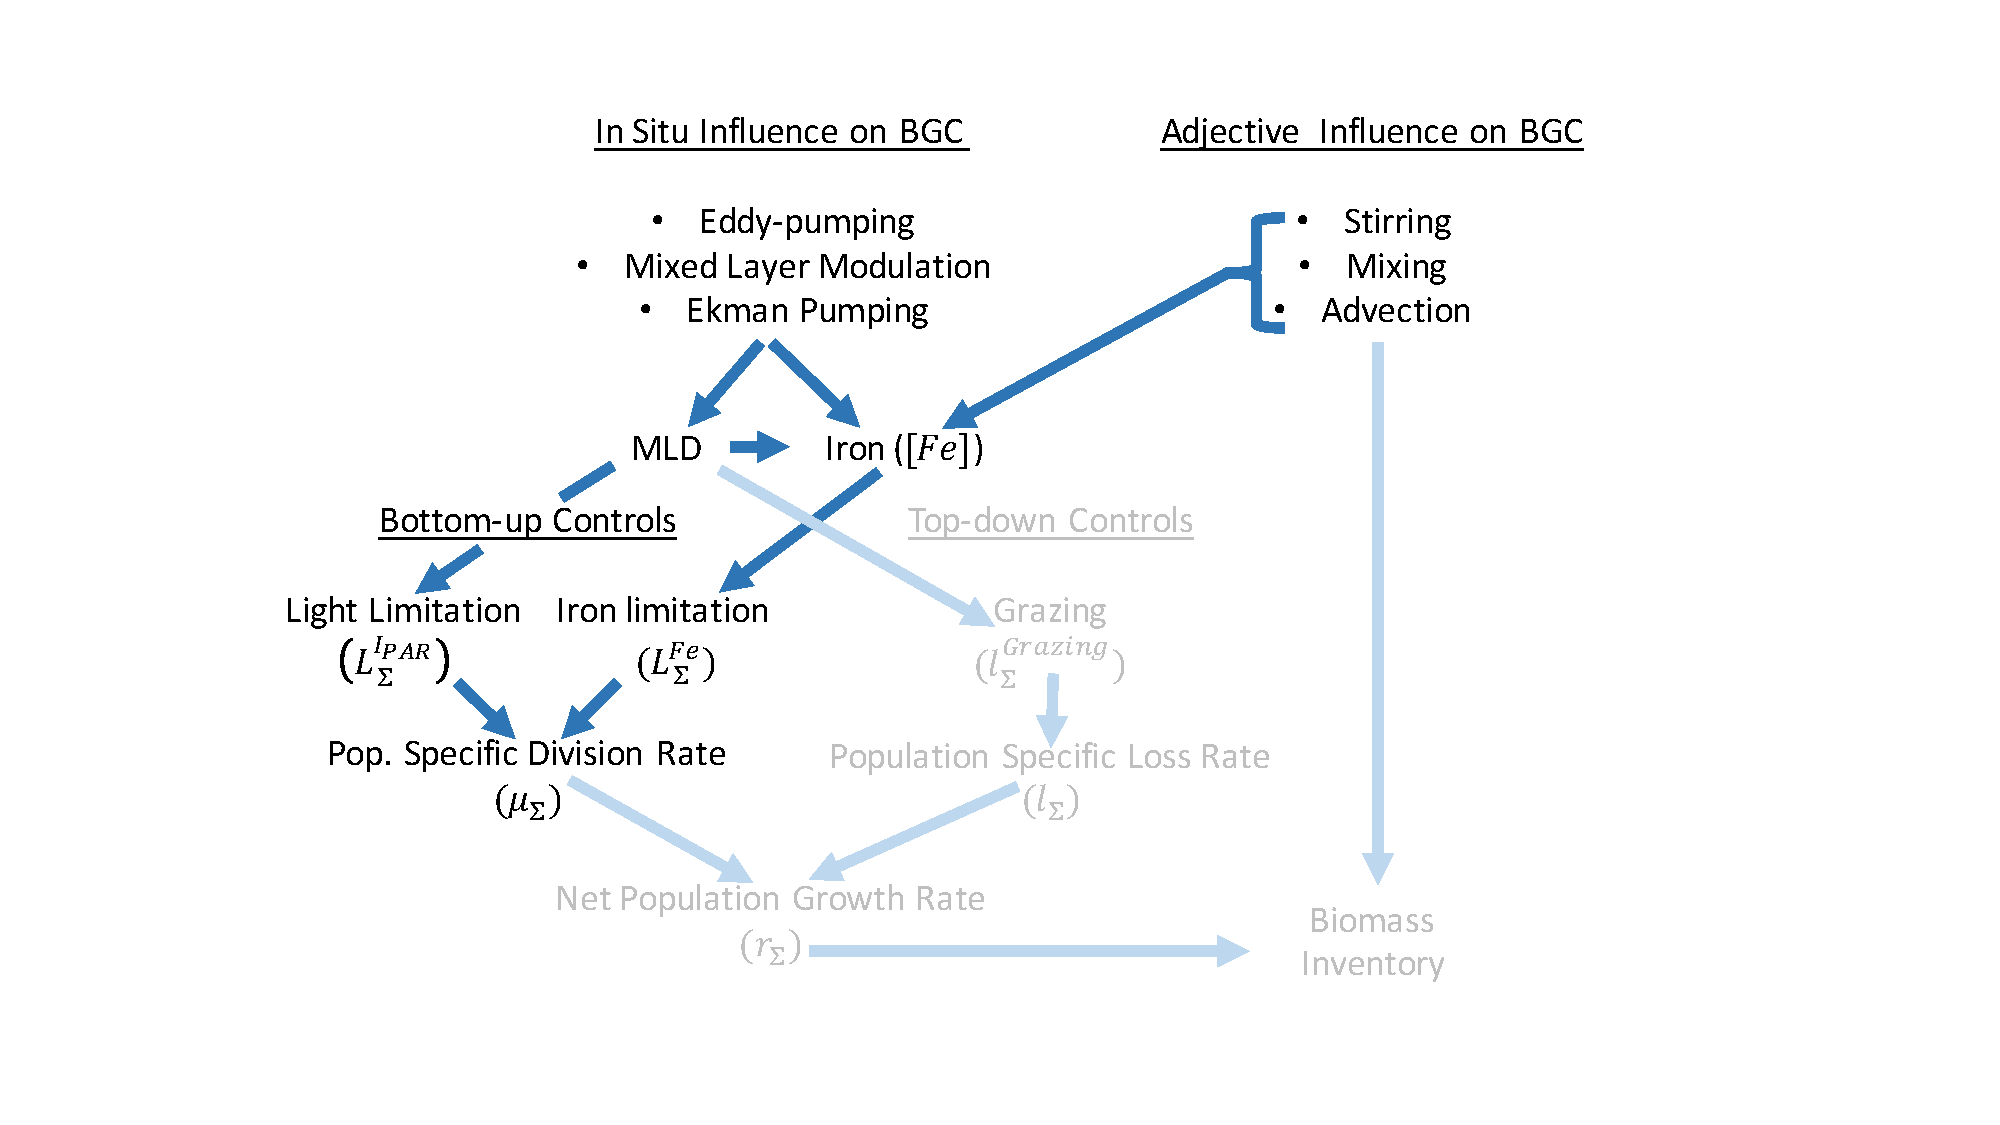
\includegraphics[scale=.8]{Fig1.pdf}
\end{adjustwidth}
\caption[Pathways for eddy influence on biomass]
{\textbf{Figure 1.} Pathways for eddy influence on biomass. Idealized flow chart of how physically induced processes in eddies can influence biogeochemistry, and ultimately biomass. Highlighted pathways and tracers are examined here. The rest are examined in \parencite{RohrEddyInducedVariabilityinprep.}}
\label{fig:Fig1}
\end{figure}

%%%%%%%%%%%%%%%%%%%%%%%%
%%%%%% Figure 2 %%%%%%%%
%%%%%%%%%%%%%%%%%%%%%%%%

\begin{figure}[!htbp]
 \begin{adjustwidth}{-.8in}{-1in}
 \centering
 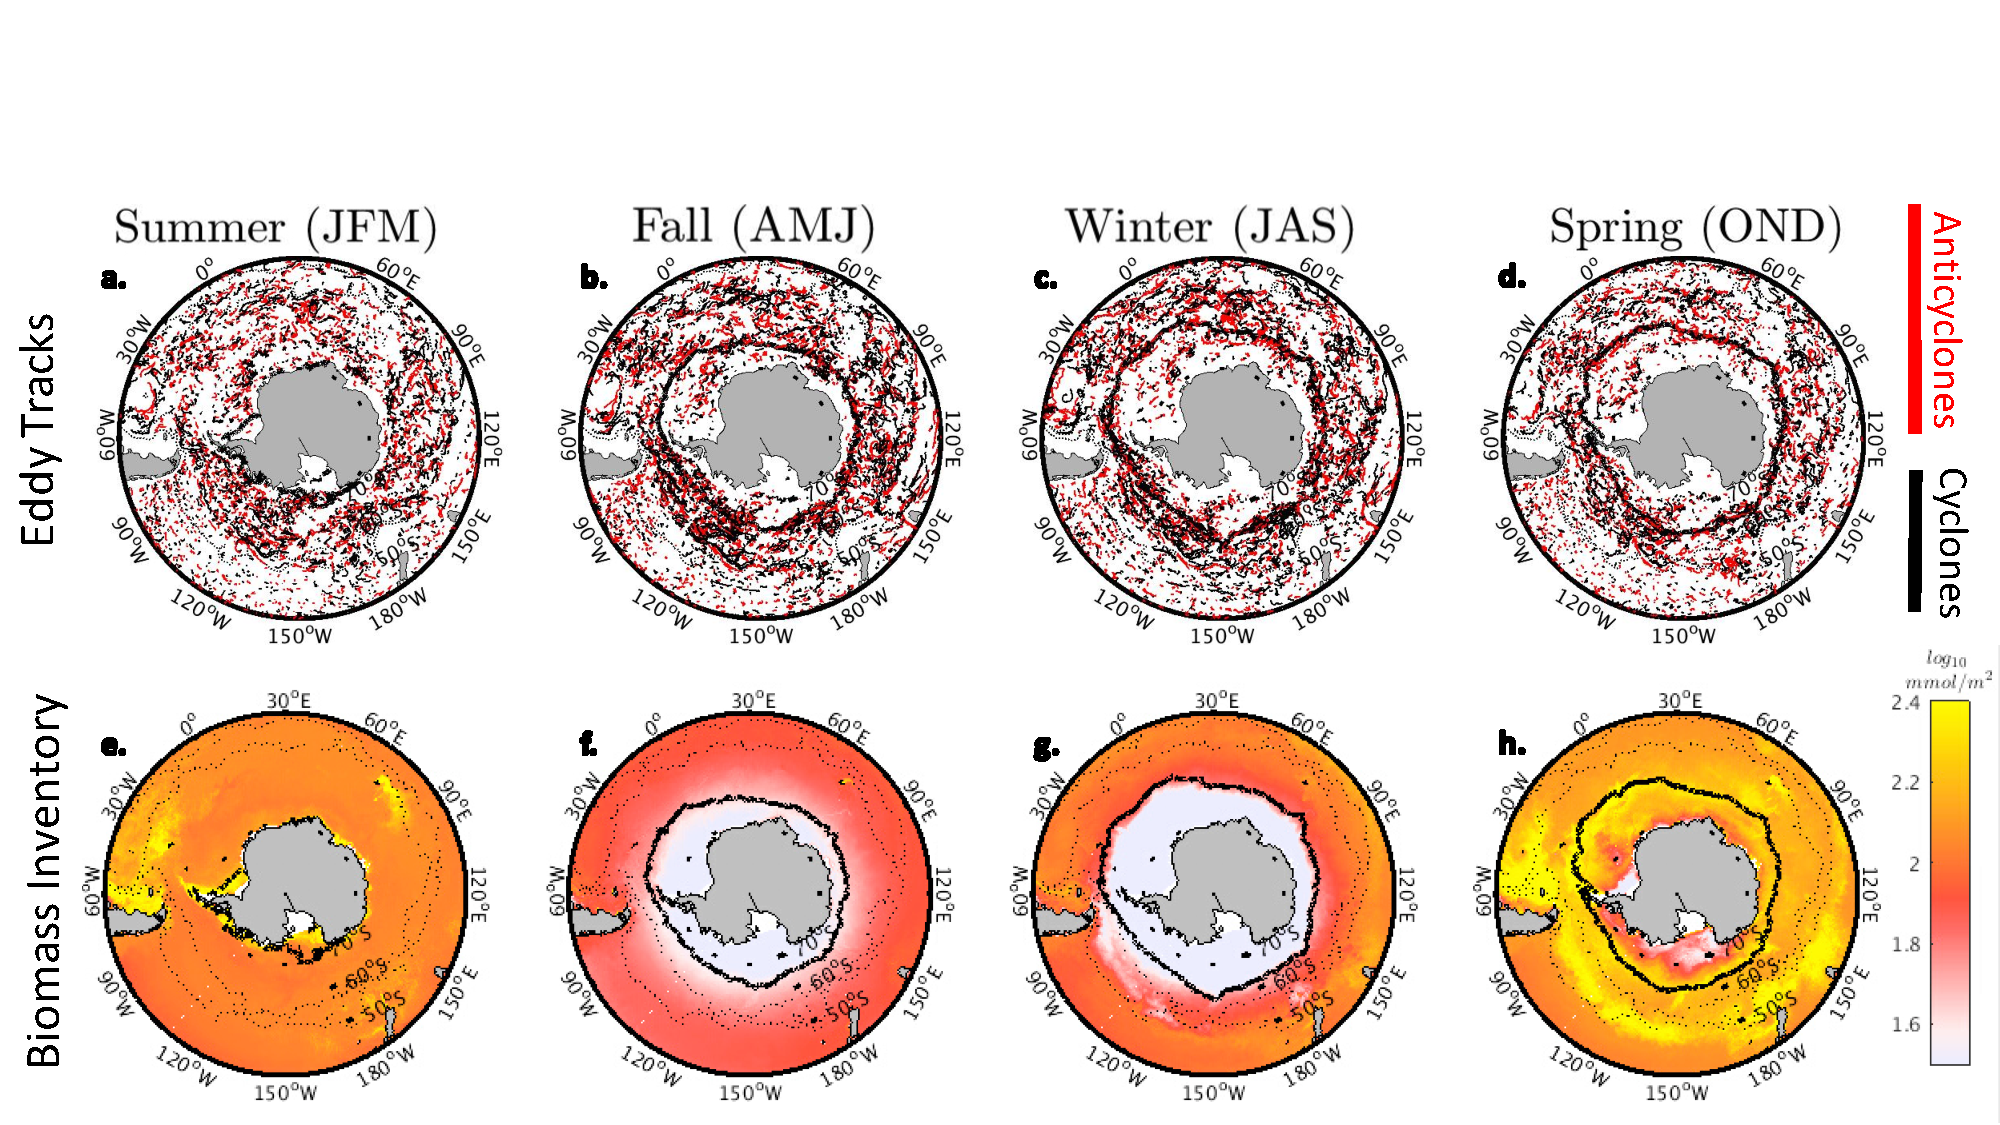
\includegraphics[scale=.6]{Fig2.pdf}
 \end{adjustwidth}
\caption[Seasonal distribution of eddy tracks and biomass inventory]
{\textbf{Figure 2.} Seasonal distribution of eddy tracks and biomass inventory. (\textbf{a-d}) The seasonal distribution of eddy tracks is plotted for cyclones (black) and anticyclones (red). Tracks are seasonally delineated by the season of their median day.  (\textbf{e-h}) The corresponding seasonal depth-integrated biomass climatology is plotted in log space. The seasonal mean 10\% ice contour is plotted in each subplot (solid black line) along with the approximated boundaries of the ACC (dashed black, $-80cm<\overline{SSH}_{Clim}<-20cm$). }
\label{fig:Fig2}
\end{figure}

%%%%%%%%%%%%%%%%%%%%%%%%
%%%%%% Figure 3 %%%%%%%%
%%%%%%%%%%%%%%%%%%%%%%%%

\begin{figure}[!htbp]
\begin{adjustwidth}{-1.2in}{-1.2in}
 \centering
 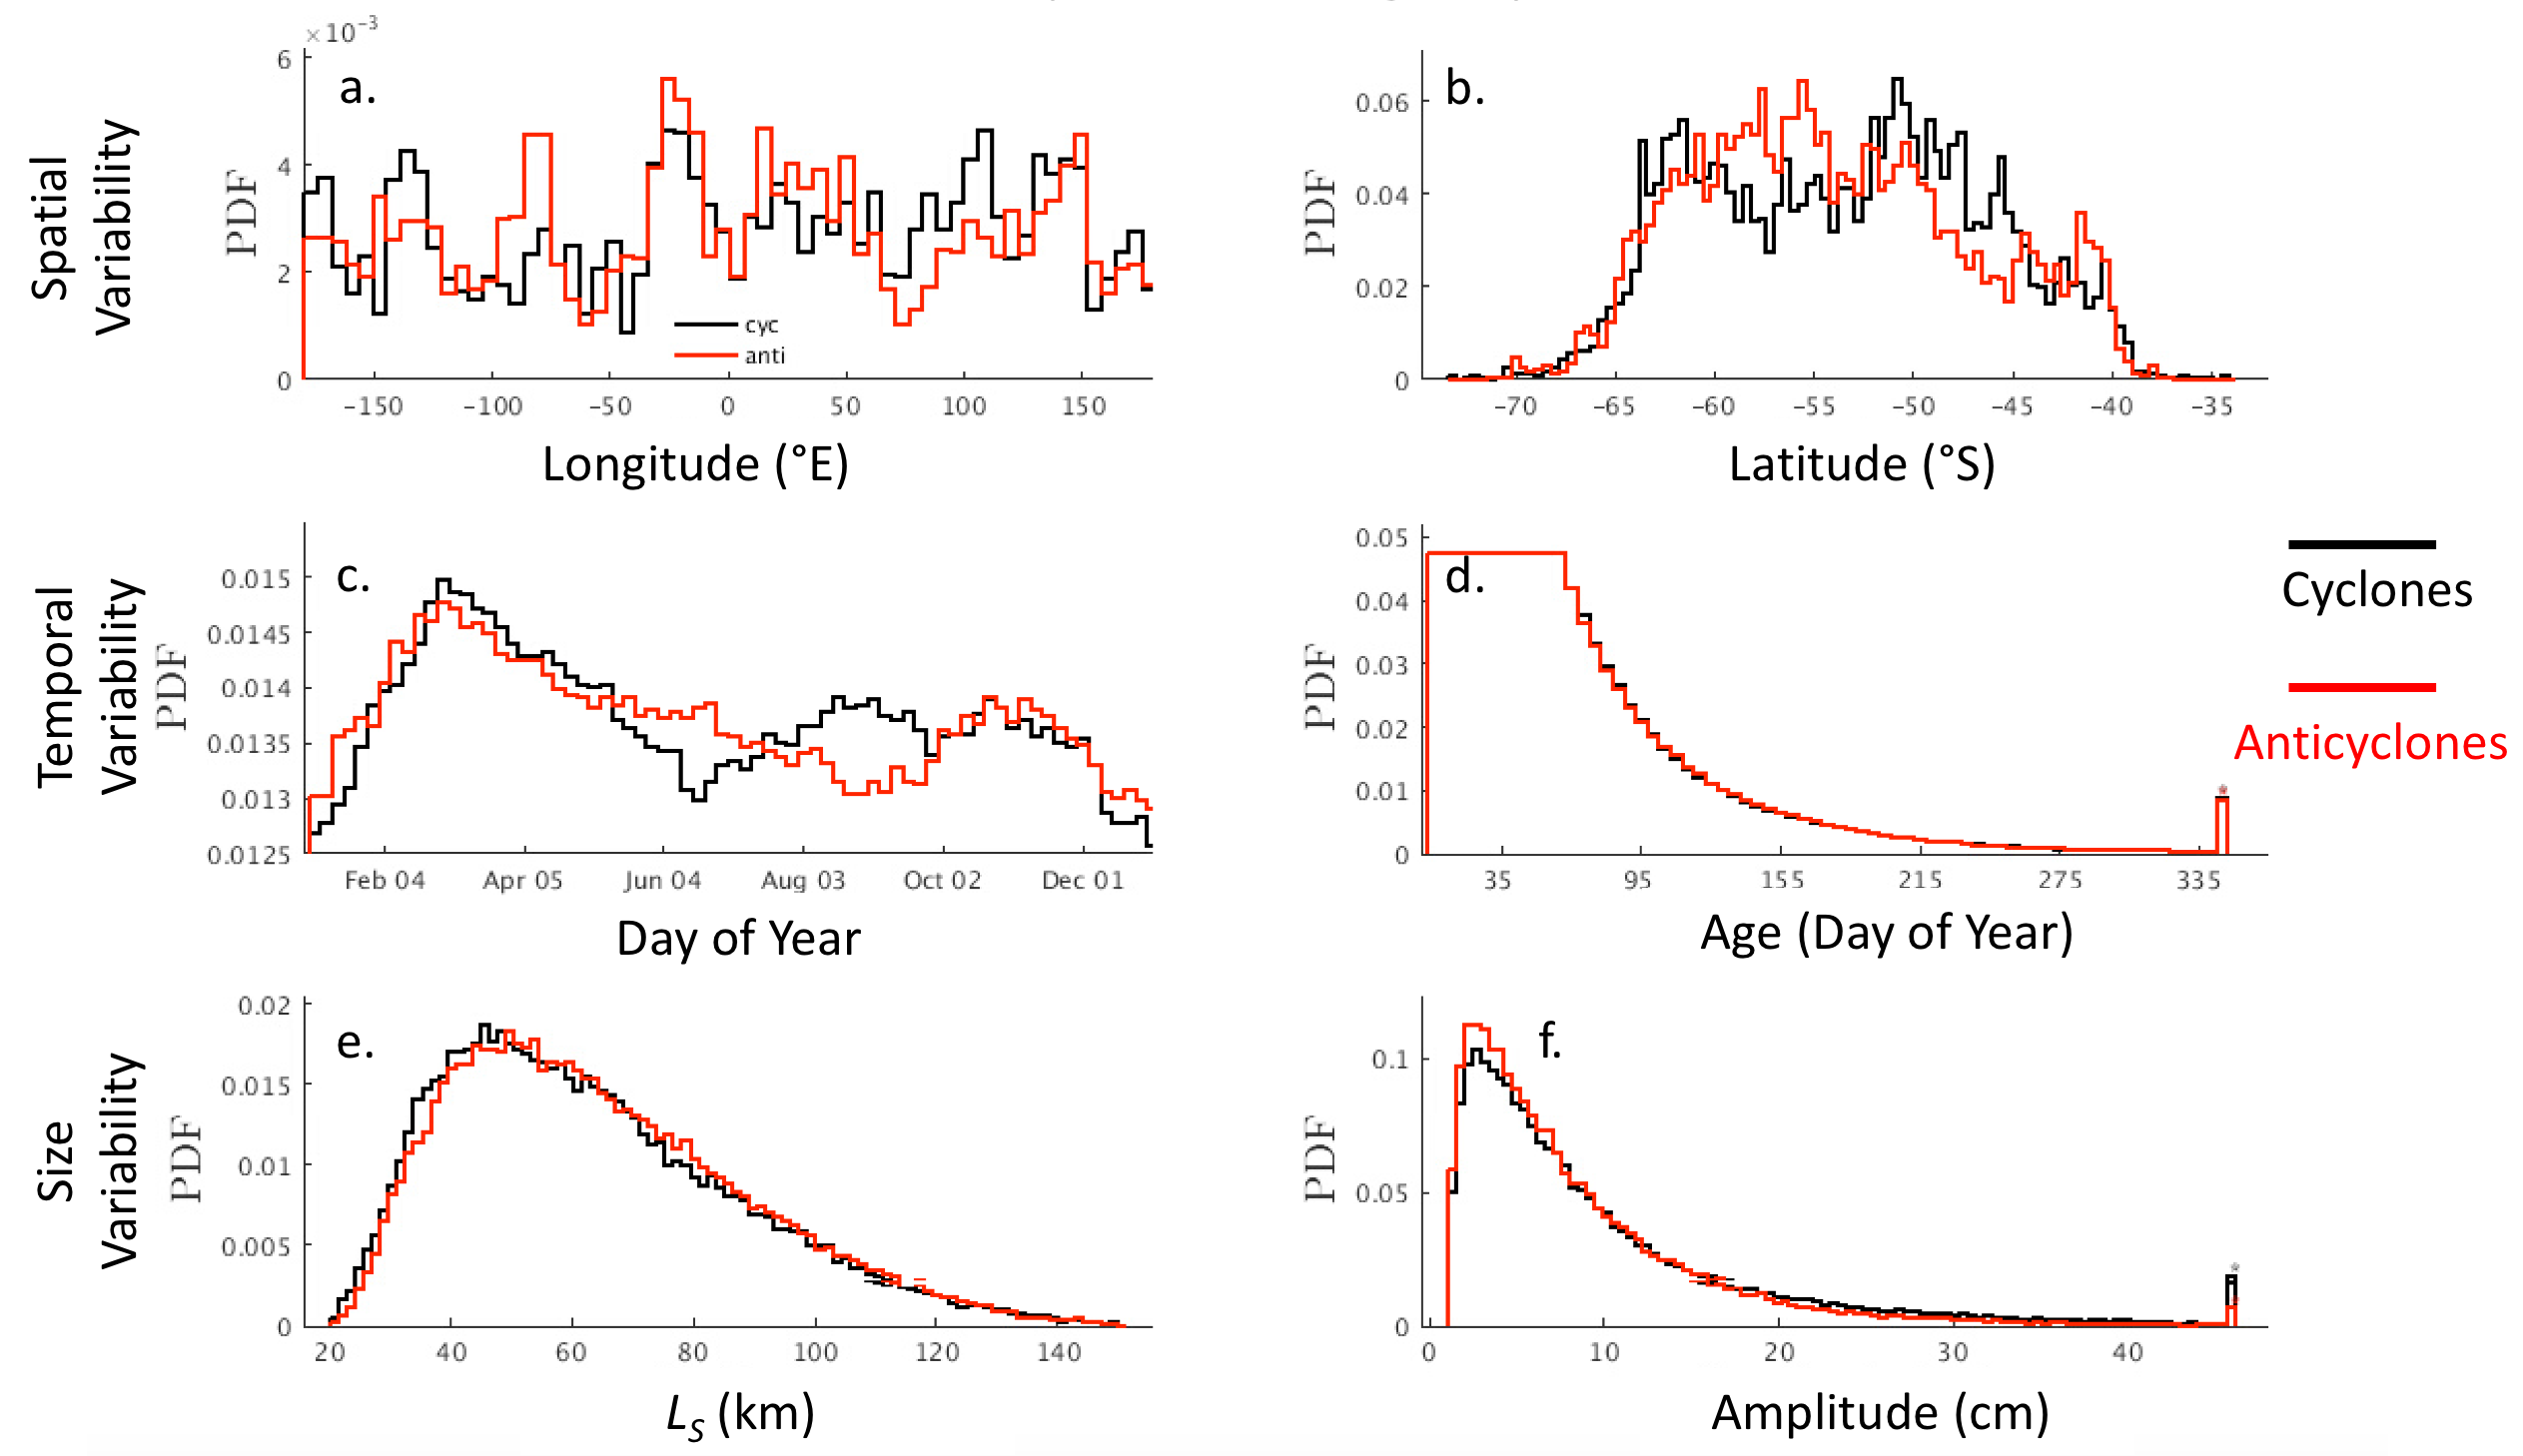
\includegraphics[scale=.40]{Fig2.png}
\end{adjustwidth}
\caption[Comparison of modeled and observed eddy demographics]
{\textbf{Figure 3.} Comparison of modeled and observed eddy demographics.  Place holder for Pete's track validation analysis. Probably something like this but with observed and simulated tracks included}
\label{fig:Fig3}
\end{figure}

%%%%%%%%%%%%%%%%%%%%%%%%
%%%%%% Figure 4 %%%%%%%%
%%%%%%%%%%%%%%%%%%%%%%%%

\begin{figure}[!htbp]
 \begin{adjustwidth}{-1.5in}{-1.2in}
 \centering
 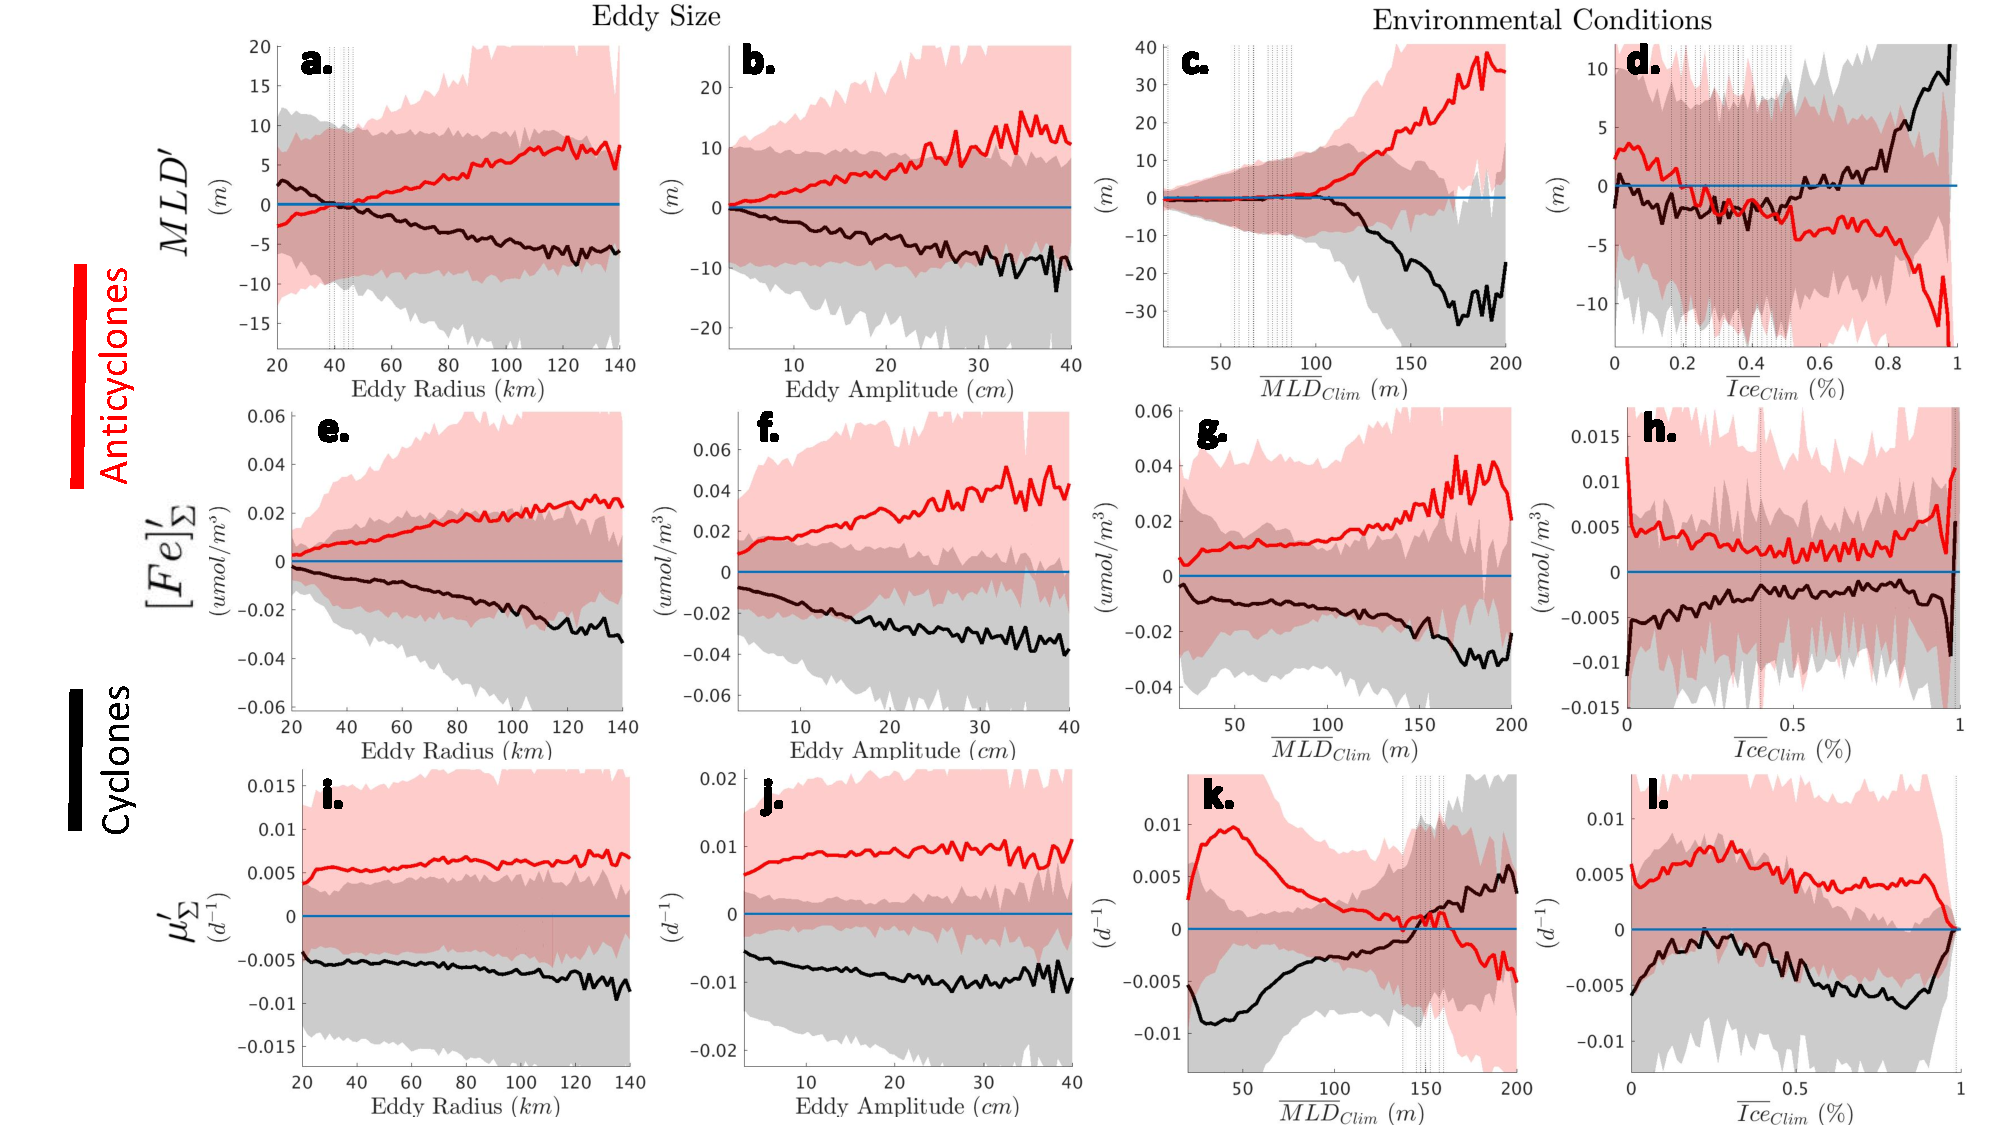
\includegraphics[scale=.60]{Fig8.pdf}
 \end{adjustwidth}
\caption[Variability in eddy anomalies]
{\textbf{Figure 4.} Variability in eddy anomalies. Variability in (\textbf{a, b, c, d}) $MLD'$,  (\textbf{e, f, g, h}) $[Fe]'_\Sigma$, and (\textbf{i, j, k, l}) $\mu'_\Sigma$ as a function of eddy radius (first column), eddy amplitude (second column), the climatologic mixed layer depth (third column) and the climatologic ice fraction (forth column). Cyclones are plotted in black. Anticyclones are plotted in red. Error bars (shaded) denotes +/- 1 standard deviation. Bins that are statistically insignificant from 0 at the 95\% confidence level are hatched out with vertical dotted lines.
}
\label{fig:Fig4}
\end{figure}



%%%%%%%%%%%%%%%%%%%%%%%%
%%%%%% Figure 5 %%%%%%%%
%%%%%%%%%%%%%%%%%%%%%%%%

\begin{figure}[!htbp]
  \begin{adjustwidth}{-1in}{-1.2in}
   \centering
    \begin{tabular}{c }
        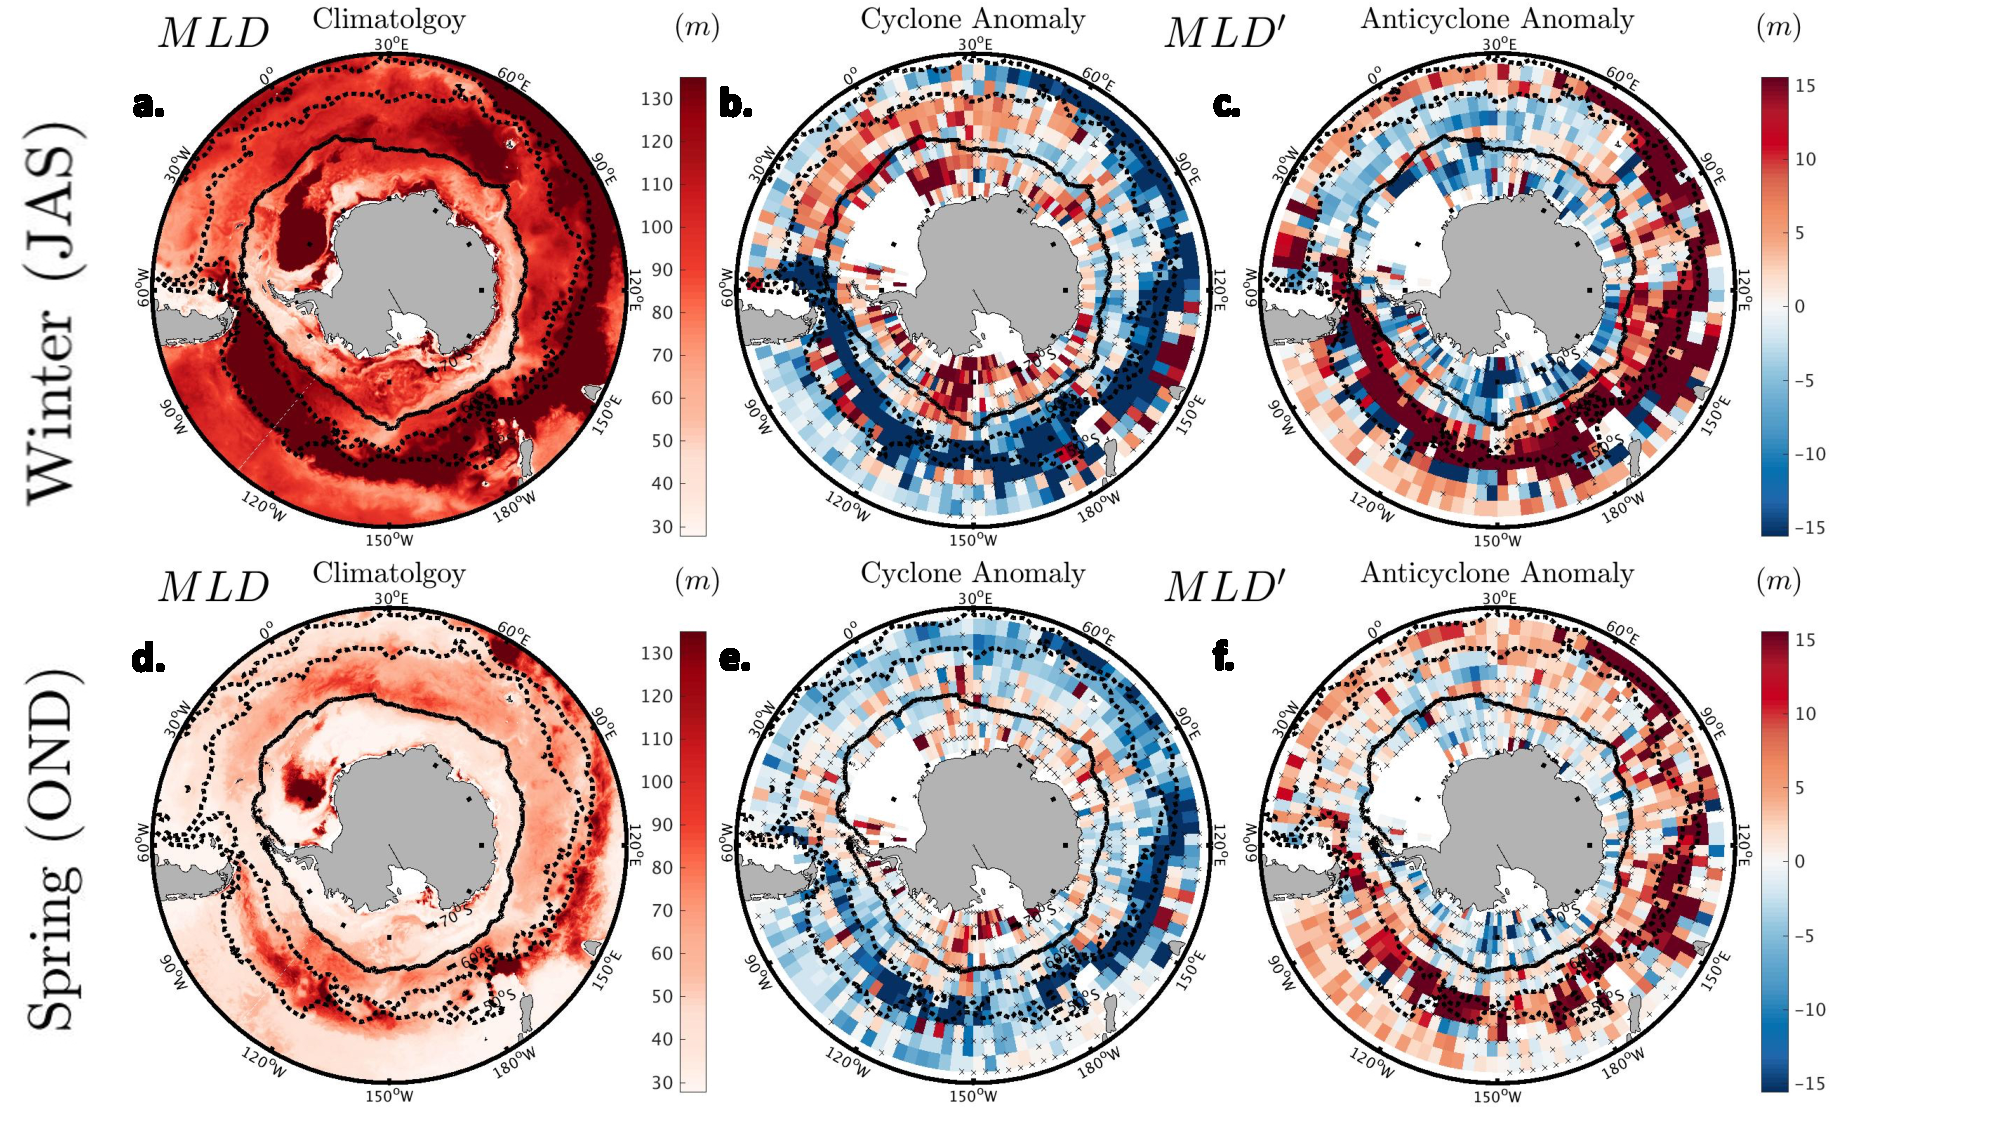
\includegraphics[scale=.5]{Fig5a.pdf} \\
        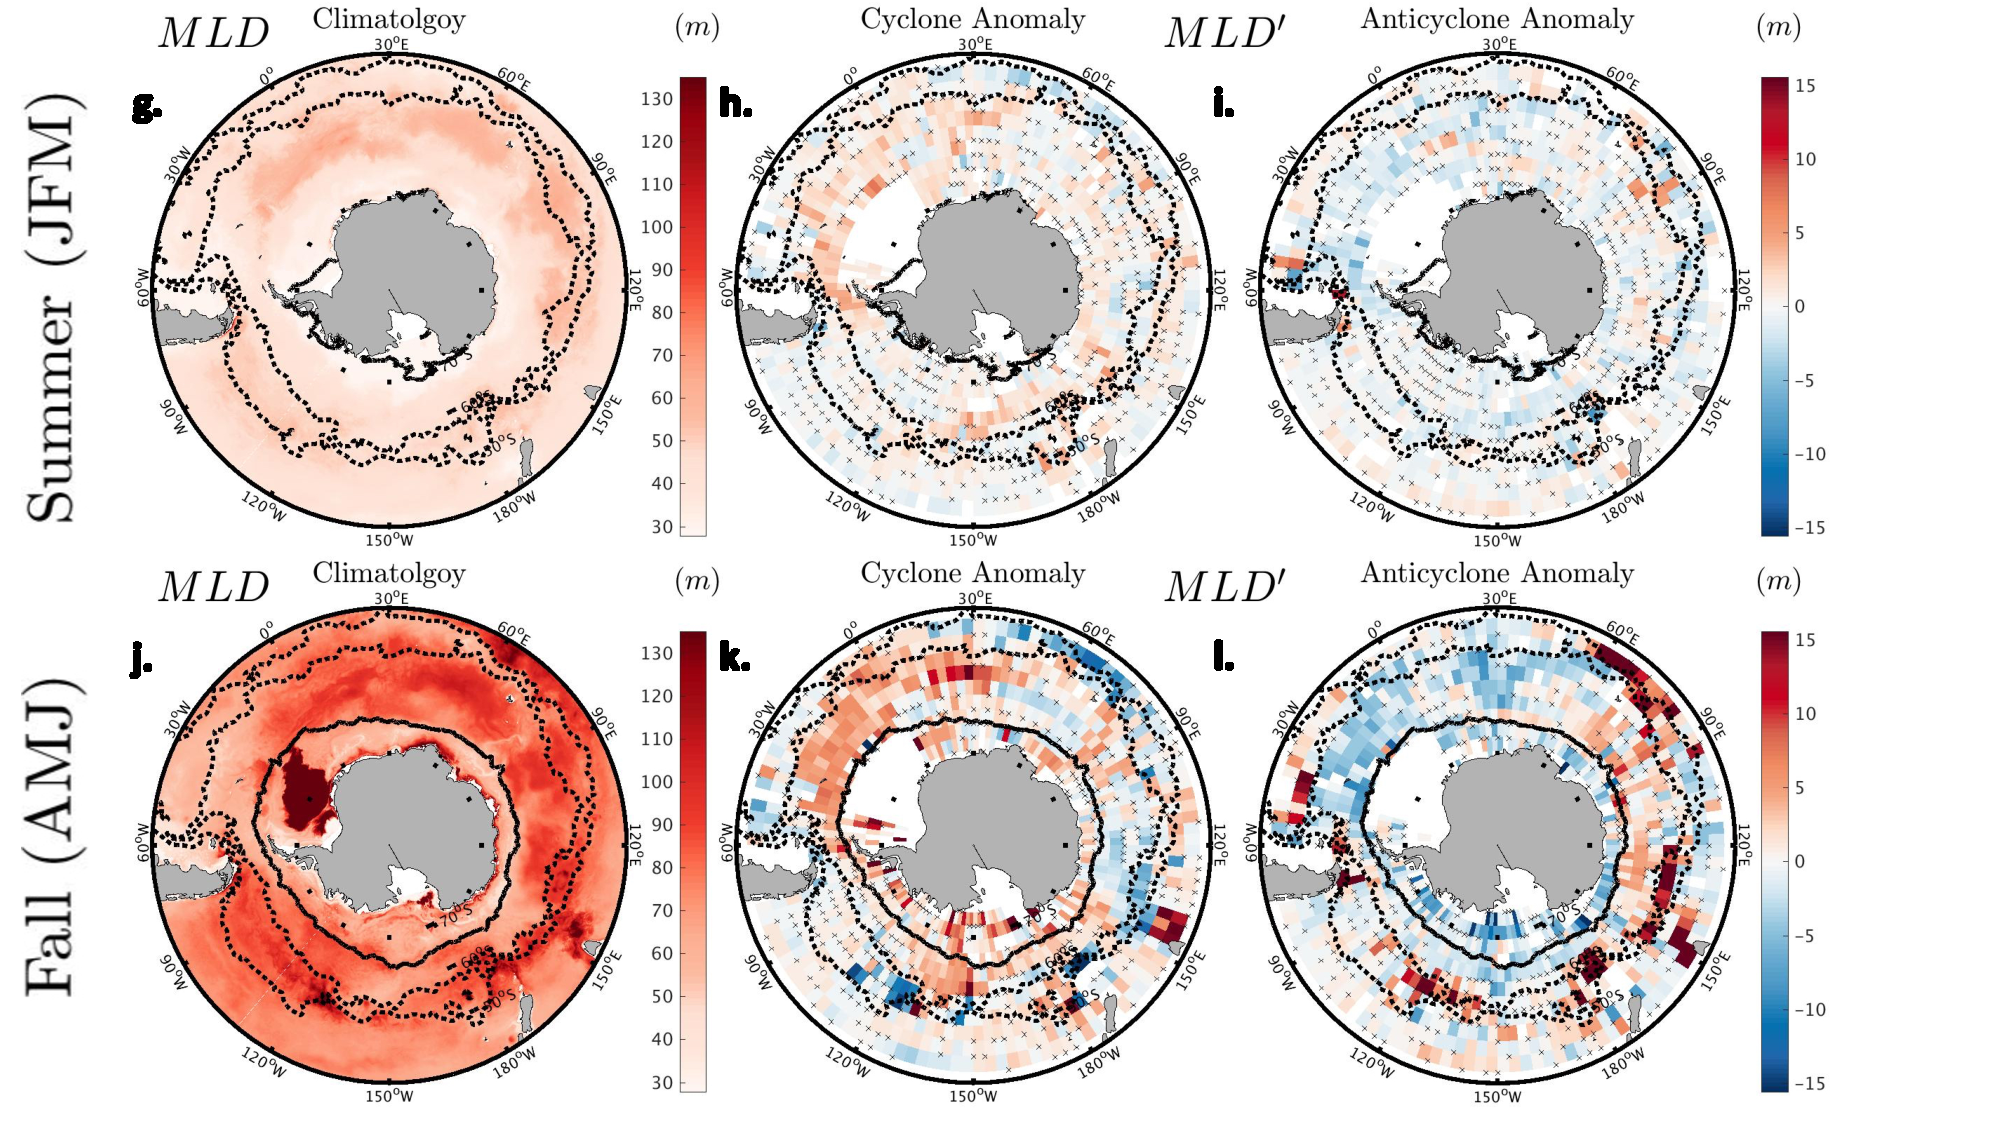
\includegraphics[scale=.5]{Fig5b.pdf} \\
    \end{tabular}
  \end{adjustwidth}
 
 
\caption[Seasonal $MLD$ climatology and eddy anomalies. ]
{\textbf{Figure 5.} Seasonal $MLD$ climatology and eddy anomalies. (\textbf{a, d, g, j}) The simulated climatologic $MLD$. (\textbf{b, e, h, k}) The simulated mean $MLD'$ in all cyclones. (\textbf{c, f, i, l}) The simulated mean $MLD'$ in all anticyclones. Data is seasonally binned as denoted in each row. Eddy realizations are further averaged over 3\degree x 3\degree spatial bins. Each bin may contain multiple realizations from the same eddy track provided that each time step falls within the seasonal threshold. Bins that are not statistically different from 0 at the 95\% confidence level are denoted with an 'x'. The 10\% ice contour is denoted in black. The ACC ($-80cm<\overline{SSH}_{Clim}<-20cm$) is denoted in with a dashed black line. 

}
\label{fig:Fig5}
\end{figure}

%%%%%%%%%%%%%%%%%%%%%%%%
%%%%%% Figure 6 %%%%%%%%
%%%%%%%%%%%%%%%%%%%%%%%%

\begin{figure}[!htbp]
 \begin{adjustwidth}{-1.2in}{-1.2in}
 \centering
  \begin{tabular}{c }
        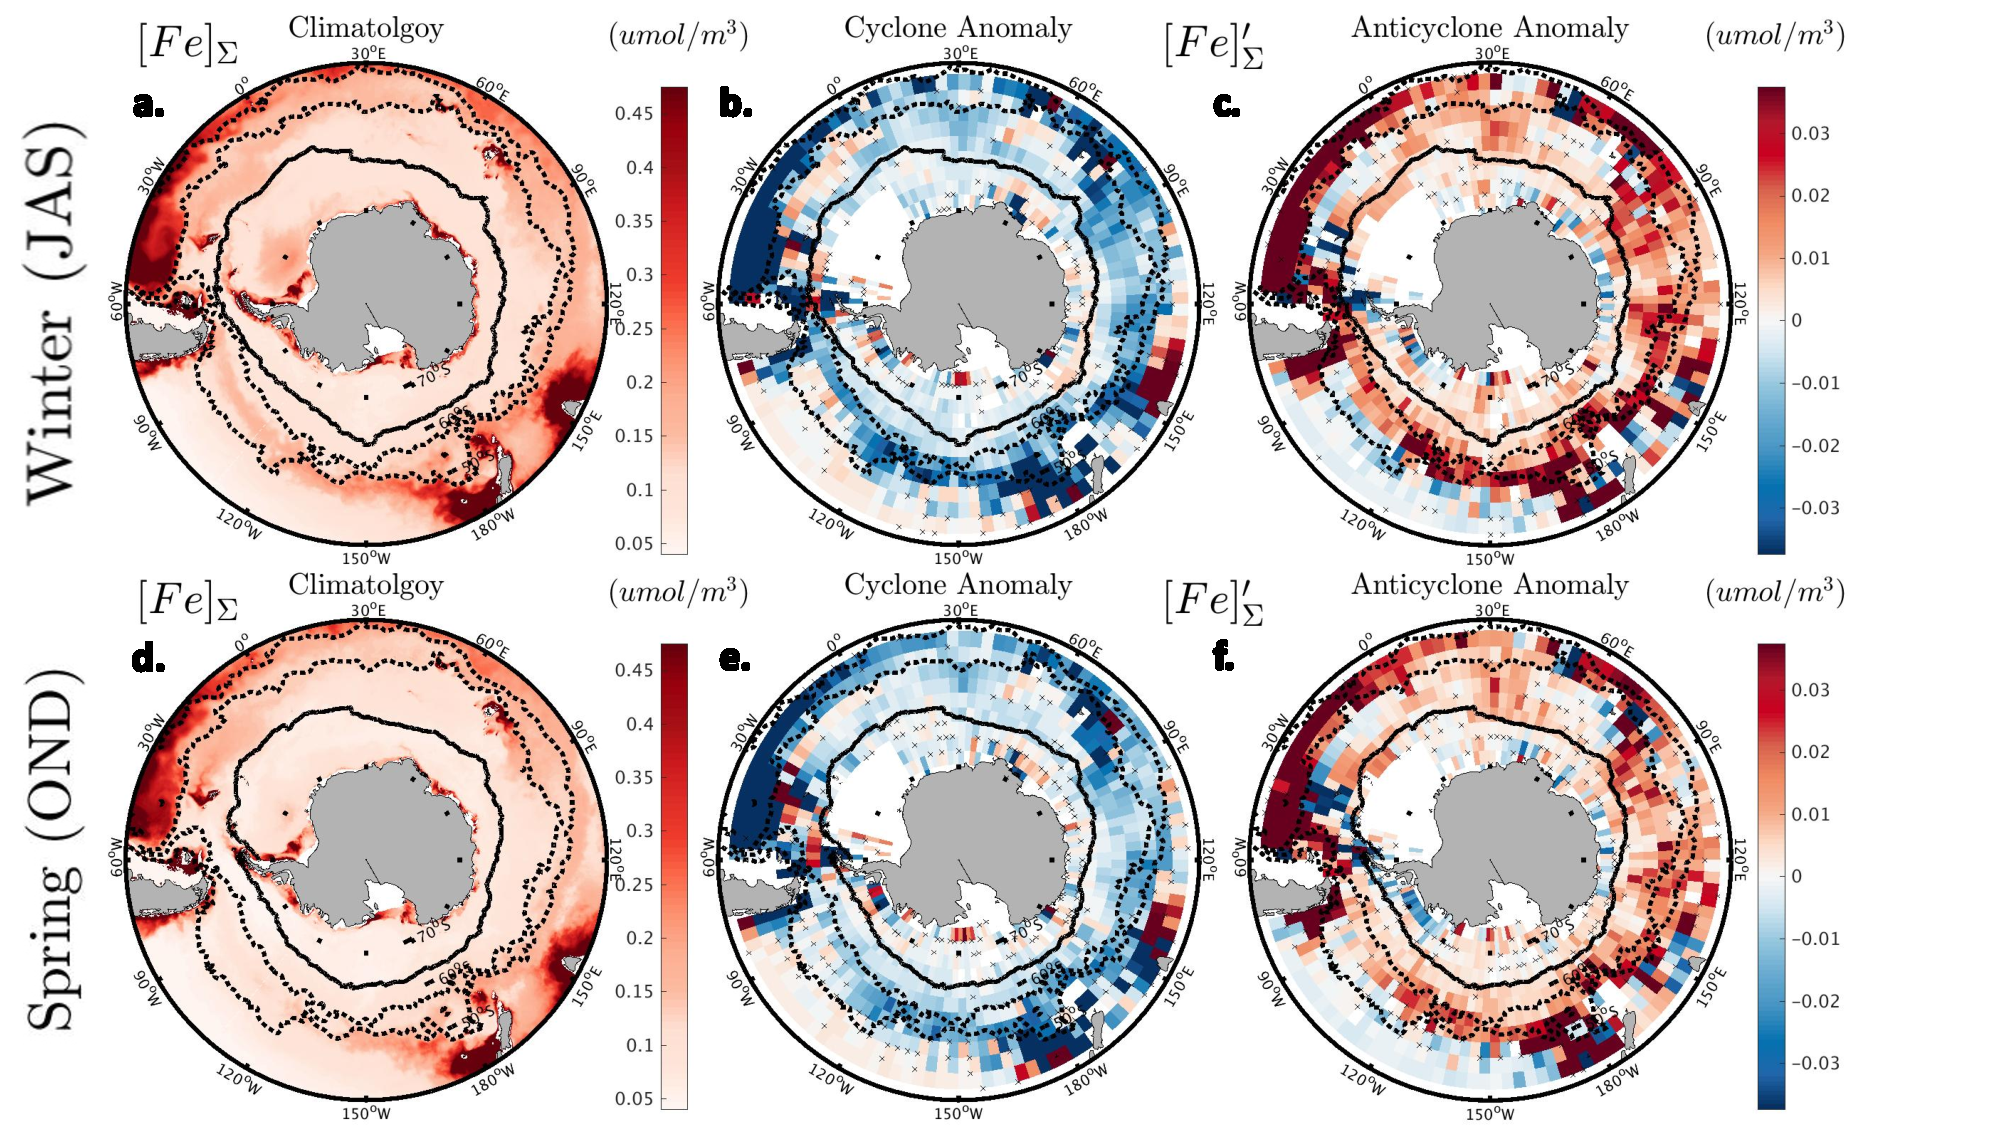
\includegraphics[scale=.5]{Fig6a.pdf} \\
        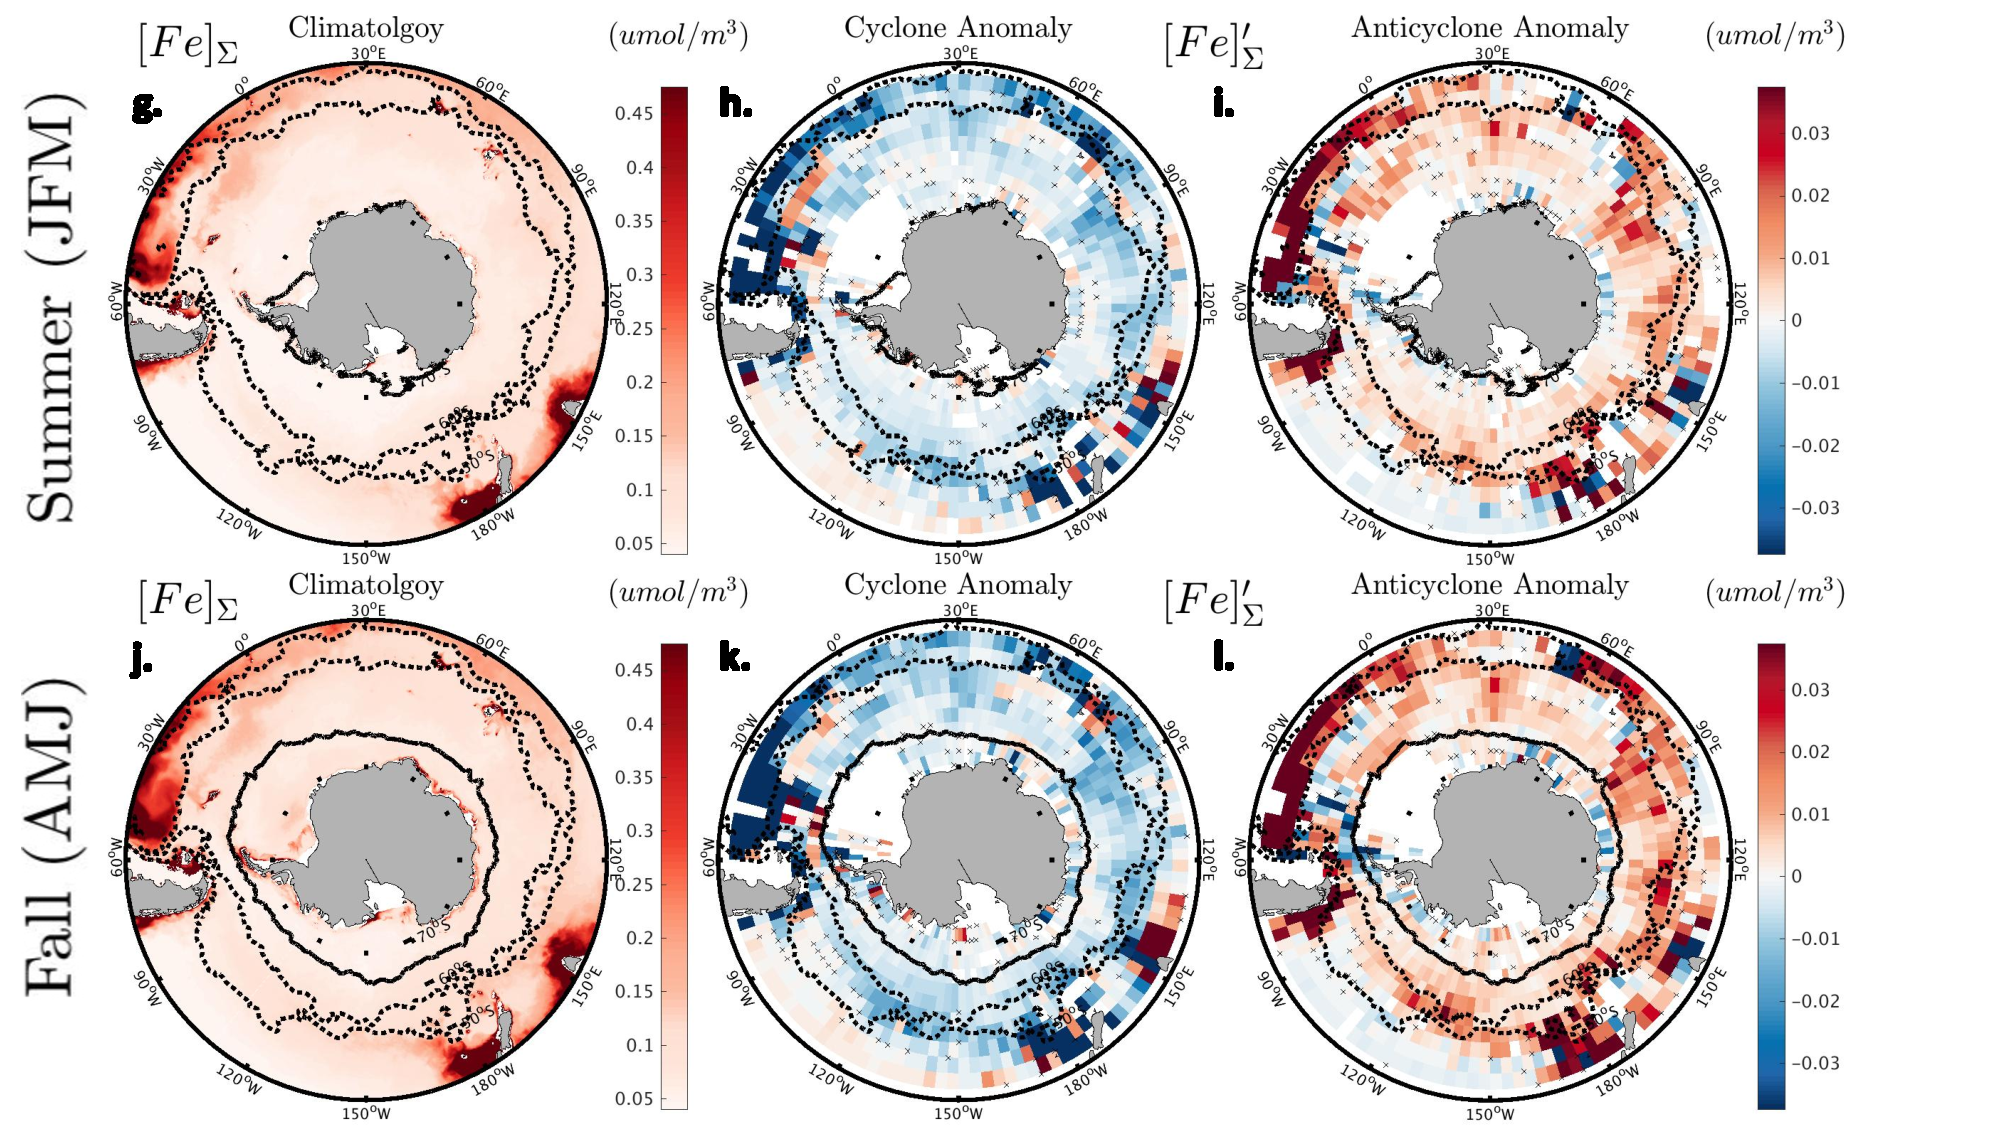
\includegraphics[scale=.5]{Fig6b.pdf} \\
  \end{tabular}
 \end{adjustwidth}
\caption[Seasonal {$[Fe]_\Sigma$} climatology and eddy anomalies.] 
{\textbf{Figure 6.} Seasonal $[Fe]_\Sigma$ climatology and eddy anomalies. Same as \textbf{Fig. 4} except for $[Fe]_\Sigma$.
}
\label{fig:Fig7}
\end{figure}

%%%%%%%%%%%%%%%%%%%%%%%%
%%%%%% Figure 7 %%%%%%%%
%%%%%%%%%%%%%%%%%%%%%%%%

\begin{figure}[!htbp]
 \begin{adjustwidth}{-1.2in}{-1.2in}
 \centering
  \begin{tabular}{c }
        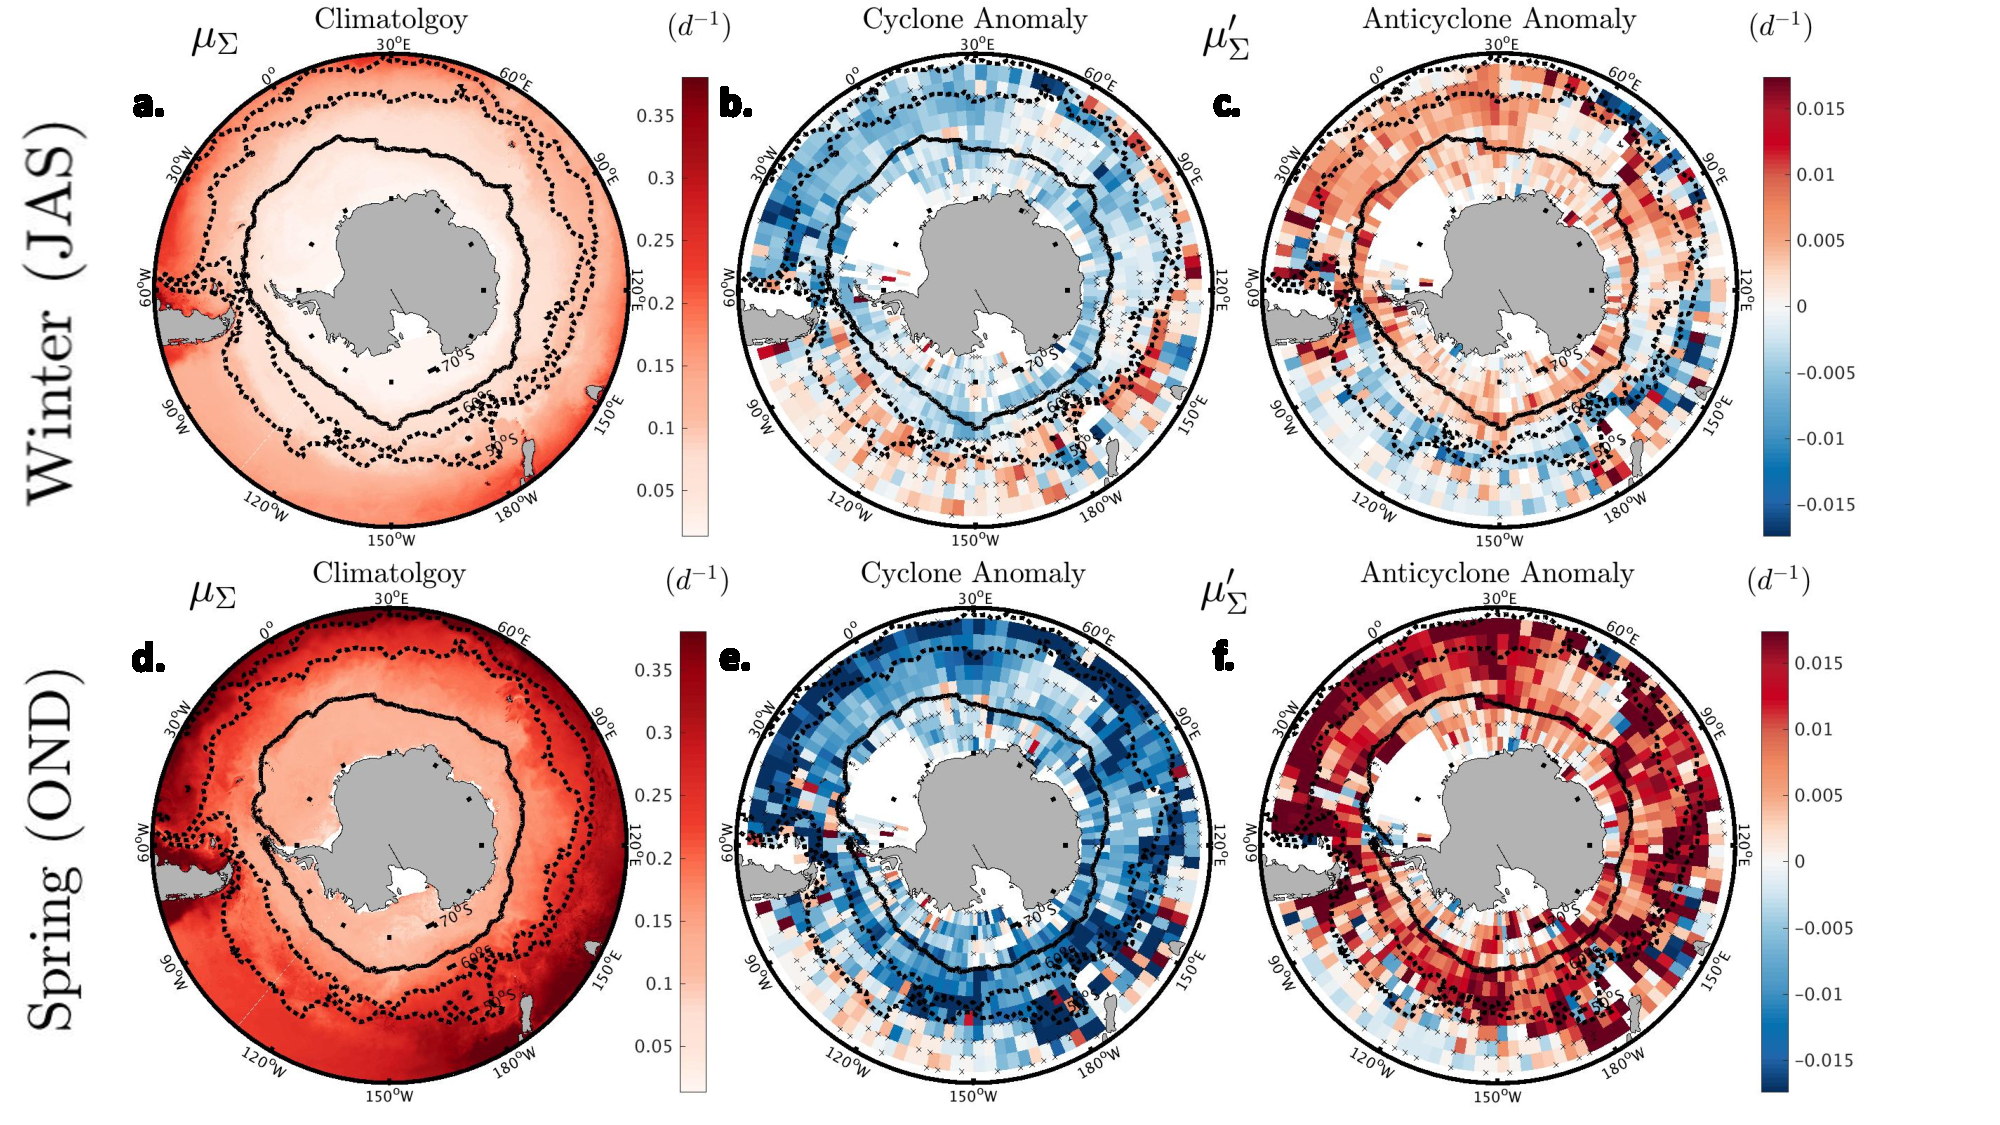
\includegraphics[scale=.5]{Fig7a.pdf} \\
        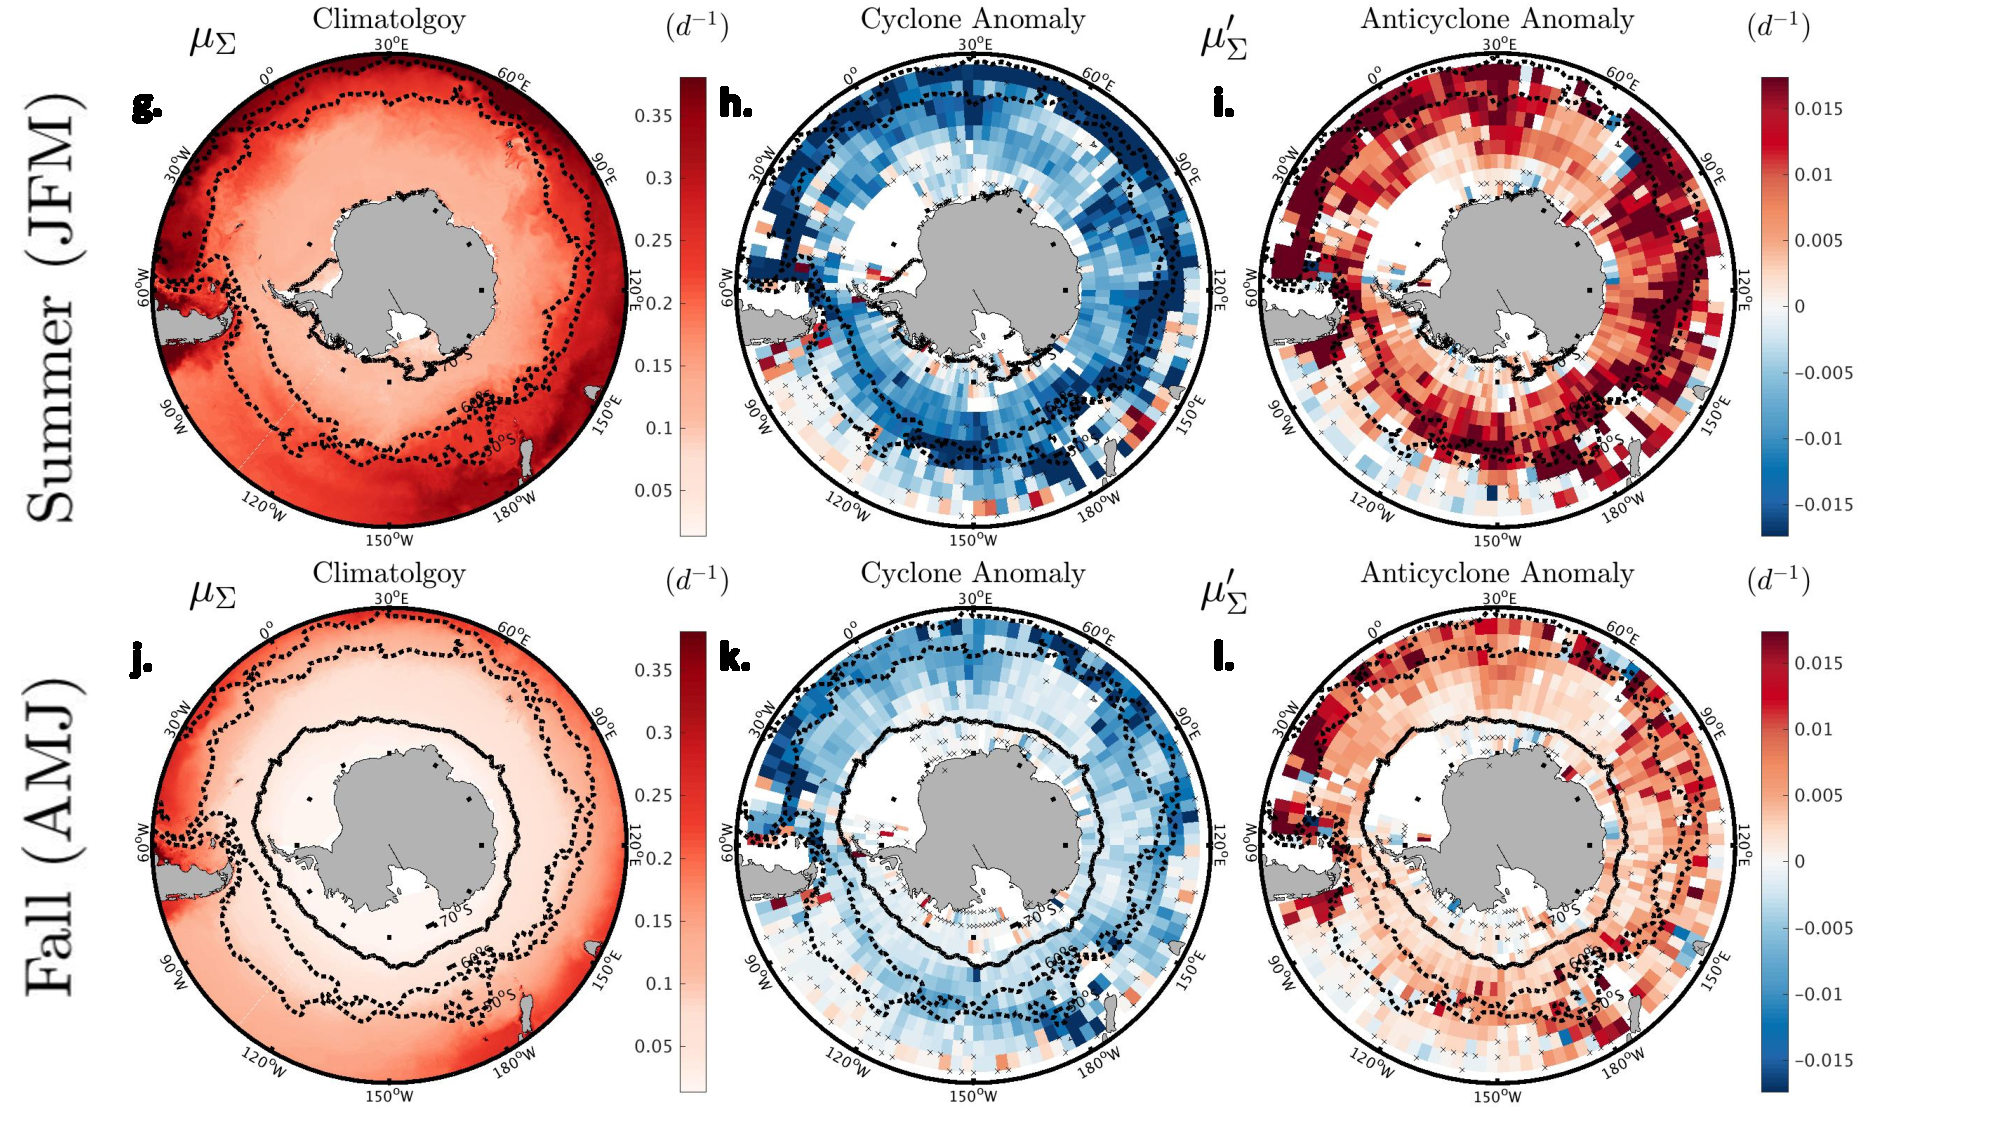
\includegraphics[scale=.5]{Fig7b.pdf} \\
  \end{tabular}
 \end{adjustwidth}
\caption[Seasonal $\mu_\Sigma$ climatology and eddy anomalies. ]
{\textbf{Figure 7.} Seasonal  $\mu_\Sigma$ climatology and eddy anomalies. Same as \textbf{Fig. 4} except for $\mu_\Sigma$.

}
\label{fig:Fig7}
\end{figure}


%%%%%%%%%%%%%%%%%%%%%%%%
%%%%%% Figure 8 %%%%%%%%
%%%%%%%%%%%%%%%%%%%%%%%%
\begin{figure}[!htbp]
\begin{adjustwidth}{-1in}{-1in}
 \centering
  \begin{tabular}{c }
        \adjincludegraphics[trim={0 0 0 {.18\height}},clip,scale=.5]{Fig8a.pdf} \\
        \adjincludegraphics[trim={0 0 0 {.18\height}},clip,scale=.5]{Fig8b.pdf} \\
    
  \end{tabular}
\end{adjustwidth}
\caption[Vertical Iron transport profiles]
{\textbf{Figure 8.} Vertical Iron transport profiles. (\textbf{a, b, c, d}) Depth profiles of the anomalous mixing flux of iron ($Mix'_Fe$) and (\textbf{e, f, g, h}) the anomalous vertical advection flux of iron  ($W'_Fe$) through bottom of each grid cell. Cyclones are plotted on the left. Anticyclones are plotted on the right. $Mix'_Fe$ is plotted as a function of (\textbf{a, b}) the background climatologic mixing depth (\overline{MLD}_{Clim}) and (\textbf{c, d}) the mixing anomaly ($MLD'$). $W'_Fe$ is plotted as a function of (\textbf{e, f}) the eddy age and (\textbf{c, d}) the anomalous Ekman velocity ($V'_{Ek}$). Bins with anomalies that are statistically insignifigant from 0 at the 95\% confidence level are marked with an '$x$'. Above each profile plot is the frequency of cyclonic (solid) and anticyclonic (dashed) eddy realizations that fall in each bin on the x-axis. Solid vertical lines delineate seasons. 
}
\label{fig:Fig8}
\end{figure}

%%%%%%%%%%%%%%%%%%%%%%%%
%%%%%% Figure 9 %%%%%%%%
%%%%%%%%%%%%%%%%%%%%%%%%

\begin{figure}[!htbp]
 \centering
  \begin{adjustwidth}{-1.8in}{-1in}
        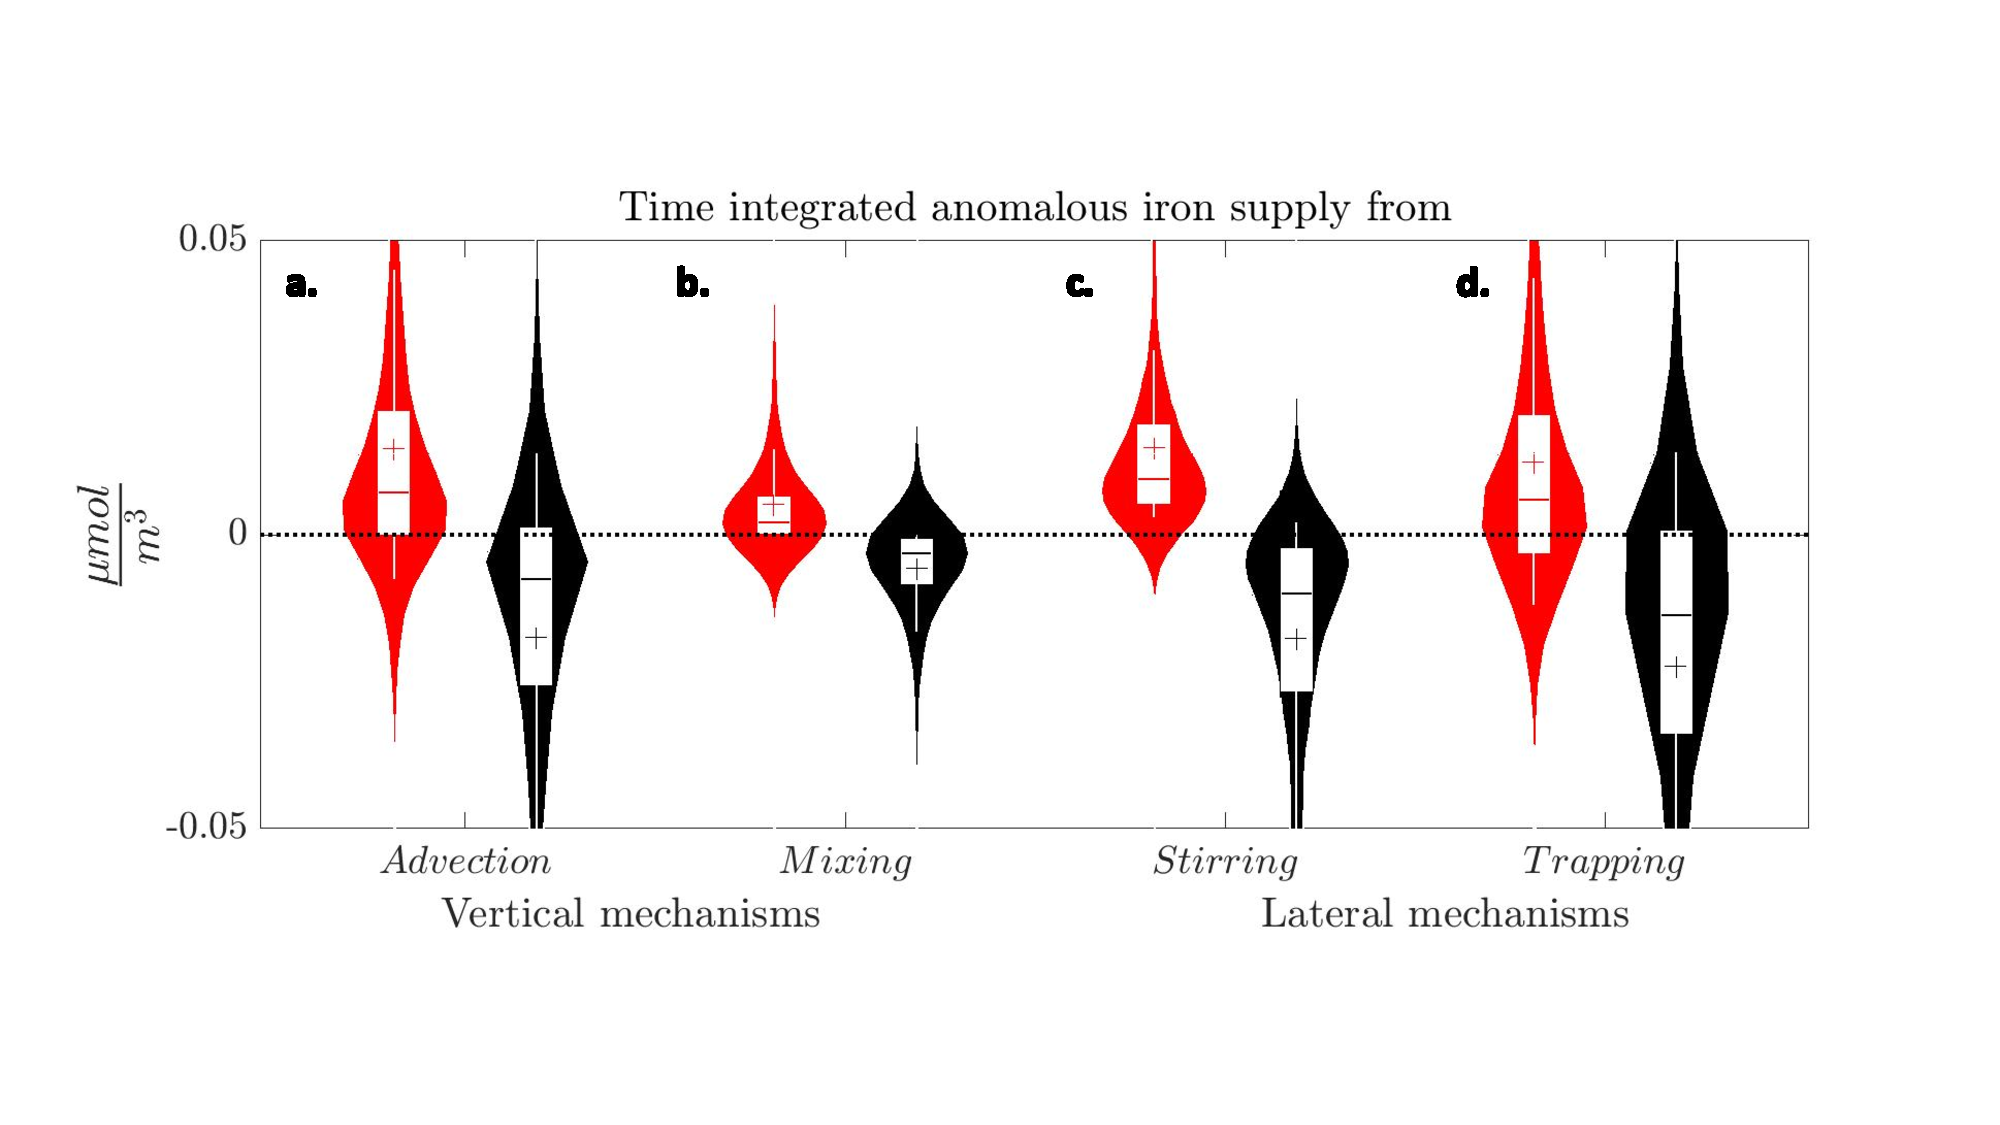
\includegraphics[scale=.74]{Fig9.pdf} \\
  \end{adjustwidth}
\caption[Iron Transport Supply ]
{\textbf{Figure 9.} Iron Transport Supply. Violin plots are provided for the anomalous time integrated community mean supply of iron in cyclones (black) and anticyclones (red) for all large eddy realizations ($L_S>50km$ \& $Amplitude>5cm$) with in the $ACC$ ($-80cm<\overline{SSH}_{Clim}<-20cm$). (\textbf{a, b}) Vertical transport mechanisms, $Advection$ and $Mixing$ quantify the actual anomalous time integrated supply of iron into the grid cell of the average phytoplankton via either mechanism over a given eddies lifetime. (\textbf{c, d}) Vertical transport mechanisms, $Stirring$ and $Trapping$, represent an estimate for the scale of and direction of anaomlies produced solely by lateral processes and is based on climatologic gradients, rather than the actualized anaomaly fields. Boxes are defined by the 25th and 75th percentile. Whiskers (white line) extend to 10th and 90th percentile. Medians are denoted with a horizonal line and means are denoted with a + symbol.
}
\label{fig:Fig9}
\end{figure}

%%%%%%%%%%%%%%%%%%%%%%%%
%%%%%% Figure 10 %%%%%%%%
%%%%%%%%%%%%%%%%%%%%%%%%

\begin{figure}[!htbp]
\vspace*{-2.5cm}
\begin{adjustwidth}{-1in}{-1in}
 \centering
 \scalebox{0.9}{
  \begin{tabular}{c }
        \adjincludegraphics[trim={0 0 0 {.17\height}},clip,scale=.5]{Fig10a.pdf} \\
        \adjincludegraphics[trim={0 0 0 {.19\height}},clip,scale=.5]{Fig10b.pdf} \\
        \adjincludegraphics[trim={{.01\width}  {.01\height} 0 {.09\height}},clip,scale=.5]{Fig10c.pdf} \\
    
  \end{tabular}
  }
\end{adjustwidth}
\caption[Seasonal variability of eddy anomalies in the deep mixing $ACC$]
{\textbf{Figure 10.} Seasonal variability of anomalies in large eddies ($L_S>50km$ \& $Amplitude>5cm$) found with in the deep mixing pacific sector of the $ACC$ ($-80cm<\overline{SSH}_{Clim}<-20cm$, $180\degree W<\textrm{LON}< 80\degree W$). Profiles of seasonal variability in $L^{I_{PAR}}'$, $L^{Fe}'$, $W'_Fe$, $Mix'_Fe$, $[C_{phyto}]'$, and $\mu'$ are plotted for cyclones on the left, and anticyclone on the right. The mean $MLD$ in cyclones (dashed) and anticyclones (solid) is overlaid. Bins with anomalies that are statistically insignificant from 0 at the 95\% confidence level are marked with an '$x$'. Above each profile plot is a plot the depth-integrated community mean value for the same variable. Bins in which the difference between cyclone and anticyclone anomalies are statistically insignificant at the 95\% confidence level are marked with a dash vertical line. Solid vertical lines delineate seasons.  
}
\label{fig:Fig10}
\end{figure}



%%%%%%%%%%%%%%%%%%%%%%%%%%%
%% Supplemental Material %%
%%%%%%%%%%%%%%%%%%%%%%%%%%%

%%%%%%%%%%%%%%%
%% Figure S1 %%
%%%%%%%%%%%%%%%

\begin{figure}[!htbp]
 \begin{adjustwidth}{-1.2in}{-1.2in}
 \centering
  \begin{tabular}{c }
        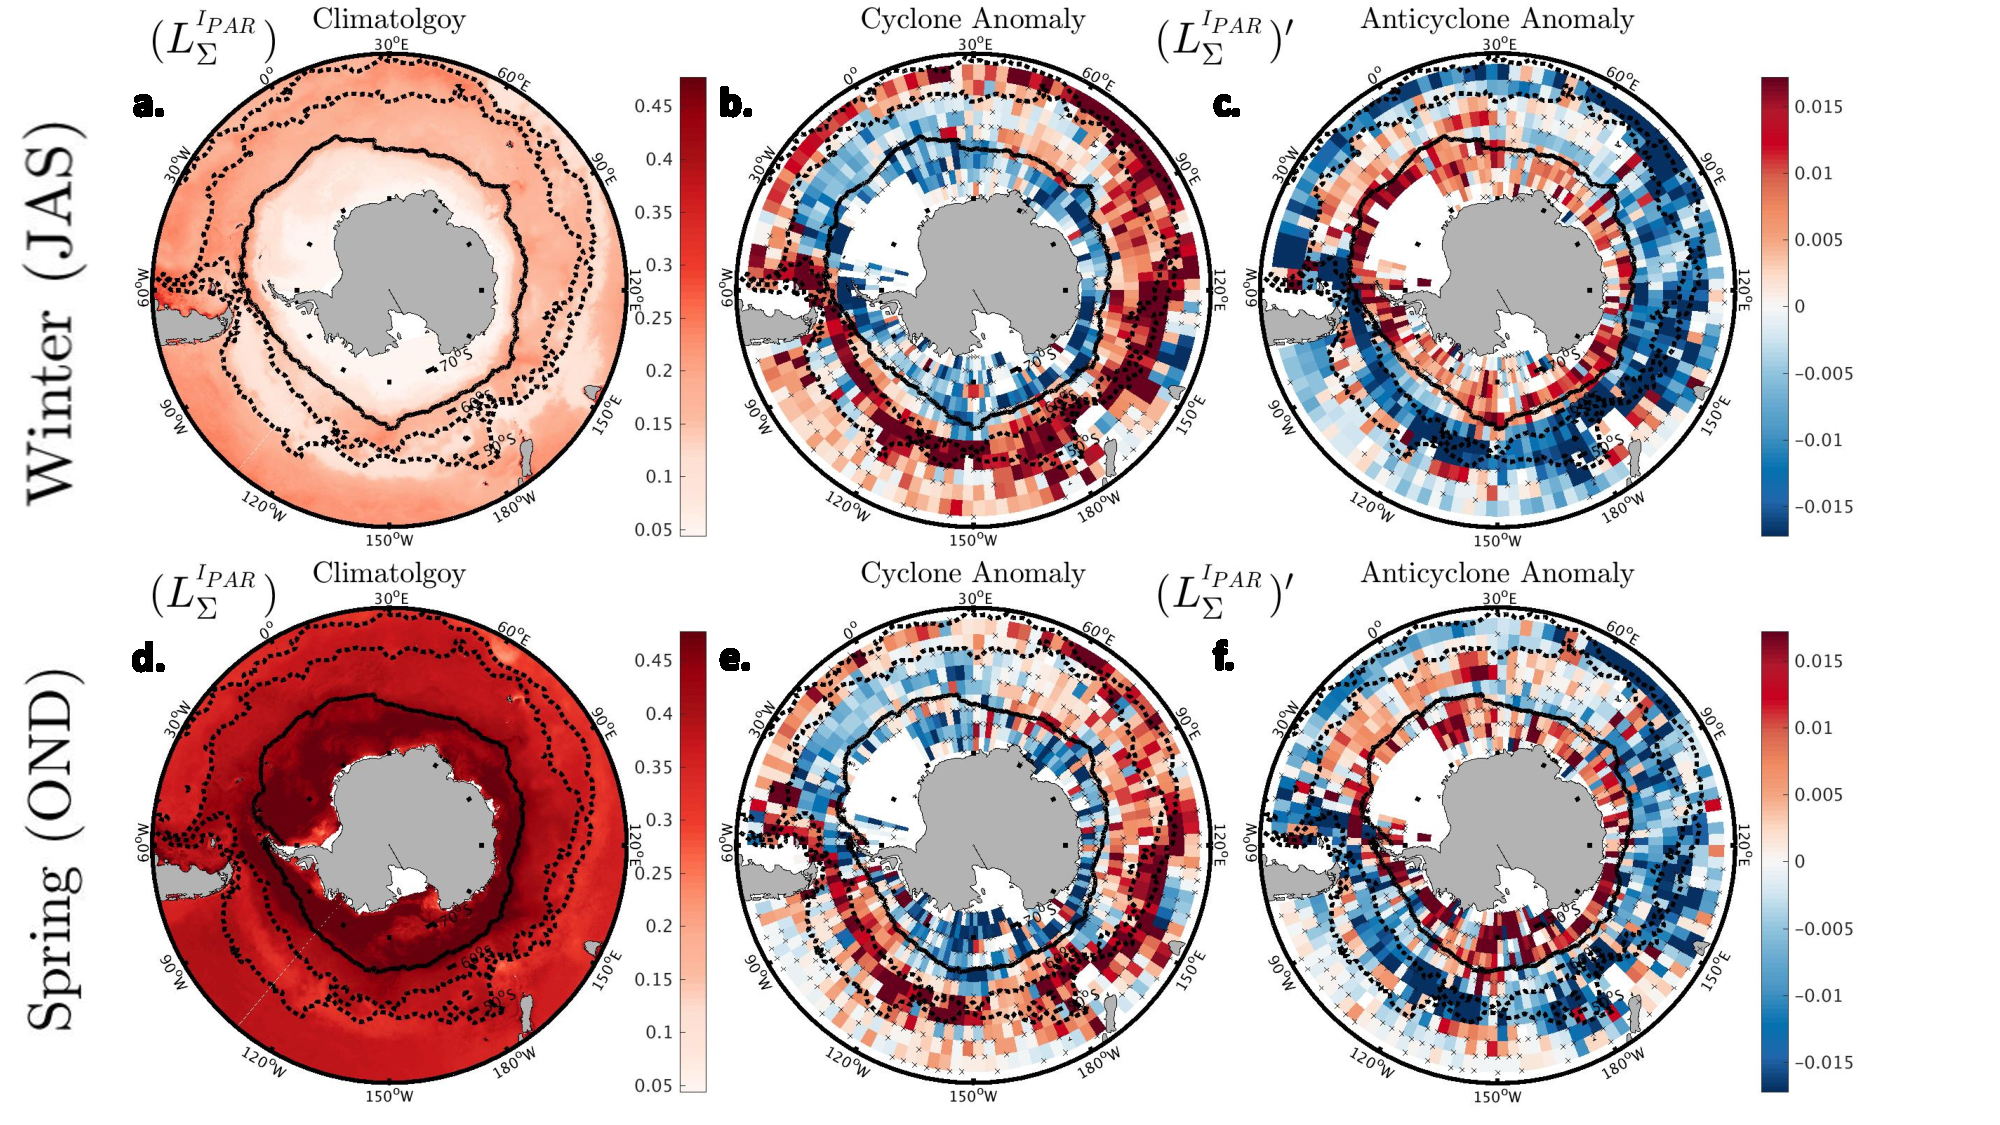
\includegraphics[scale=.5]{FigS4a.pdf} \\
        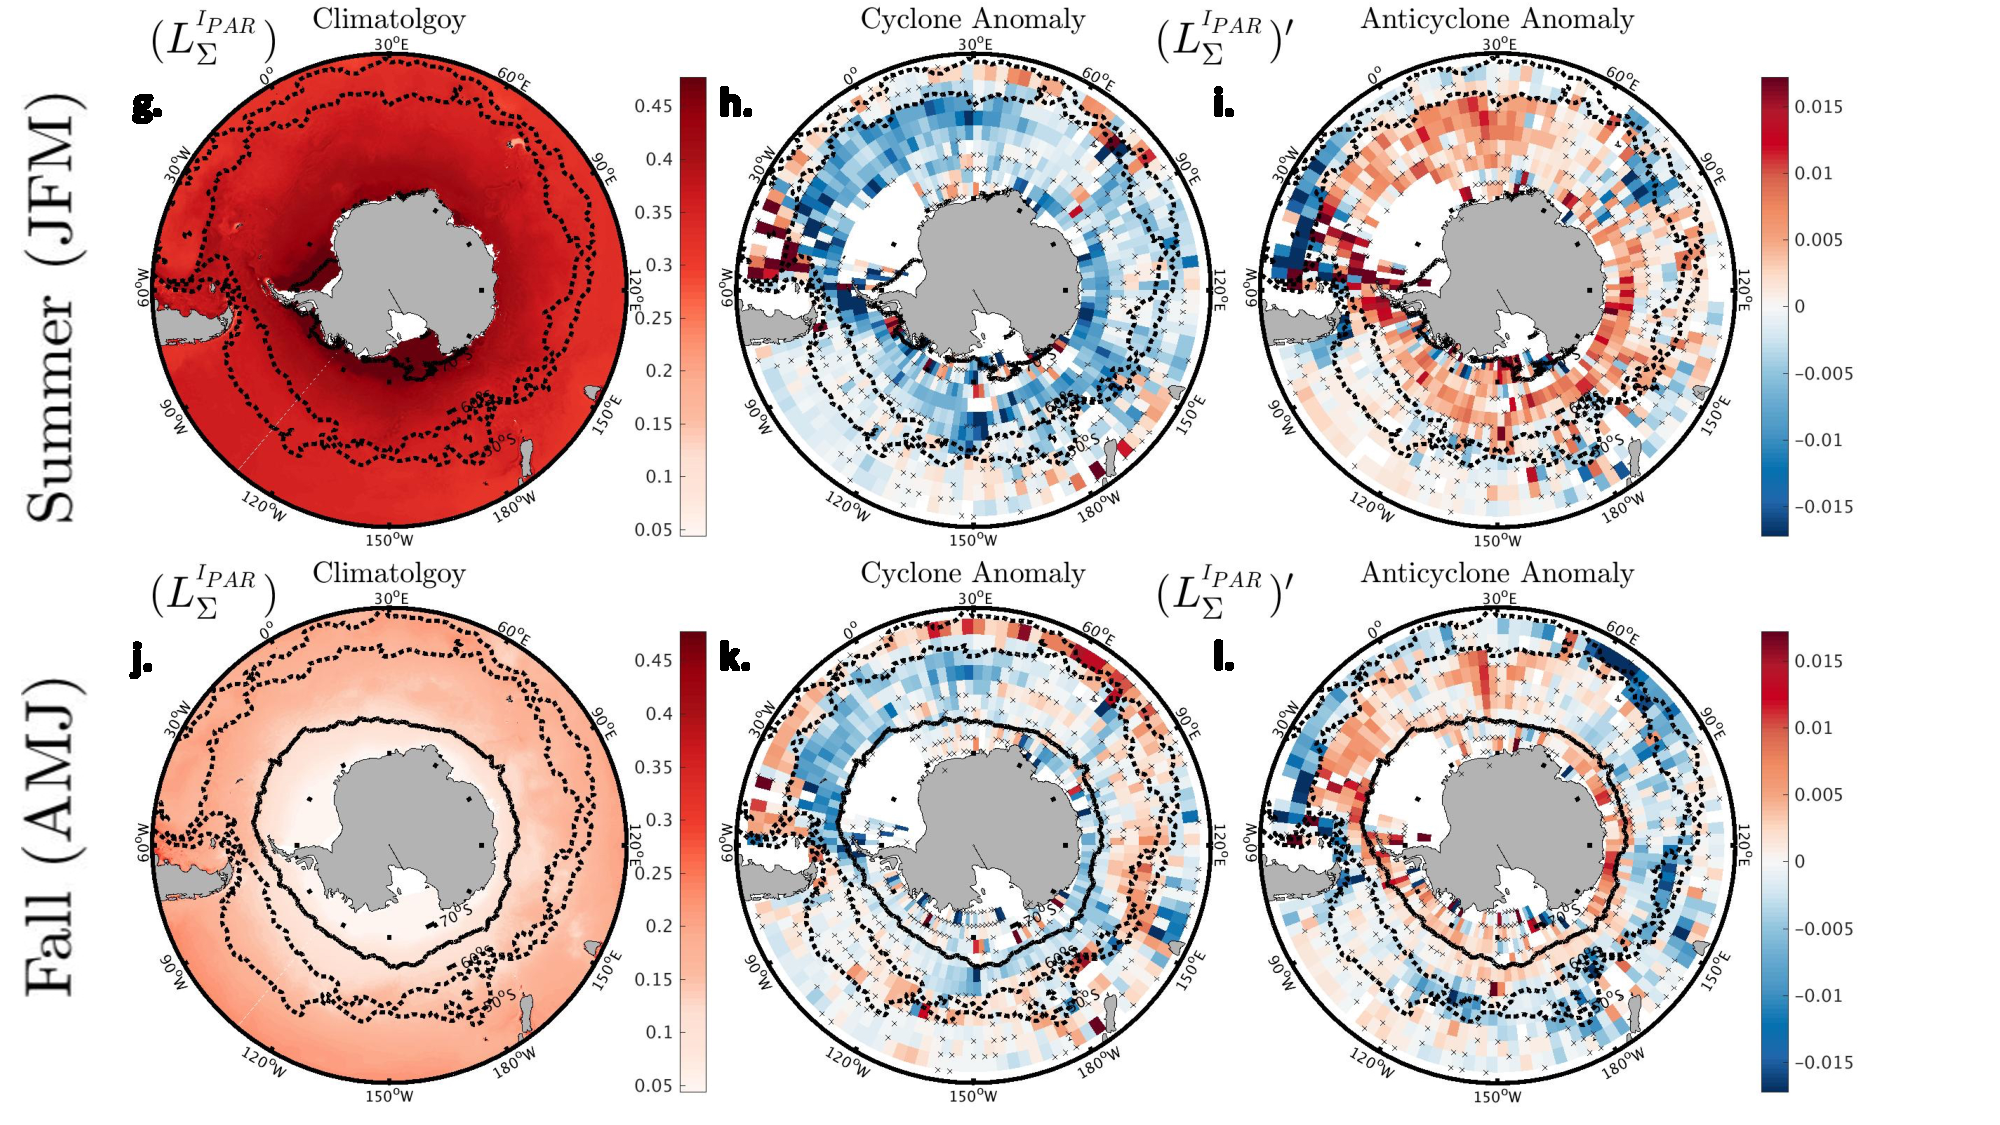
\includegraphics[scale=.5]{FigS4b.pdf} \\
  \end{tabular}
 \end{adjustwidth}
\caption[S1. Seasonal  $L_\Sigma^{I_{PAR}}'$ climatology and eddy anomalies. ]
{\textbf{Figure S1.} Seasonal  $L_\Sigma^{I_{PAR}}$ climatology and eddy anomalies. Same as \textbf{Fig. 4} except for $L_\Sigma^{I_{PAR}}$.
}
\label{fig:FigS1}
\end{figure}


%%%%%%%%%%%%%%%
%% Figure S2 %%
%%%%%%%%%%%%%%%

\begin{figure}[!htbp]
 \begin{adjustwidth}{-1.2in}{-1.2in}
 \centering
  \begin{tabular}{c }
        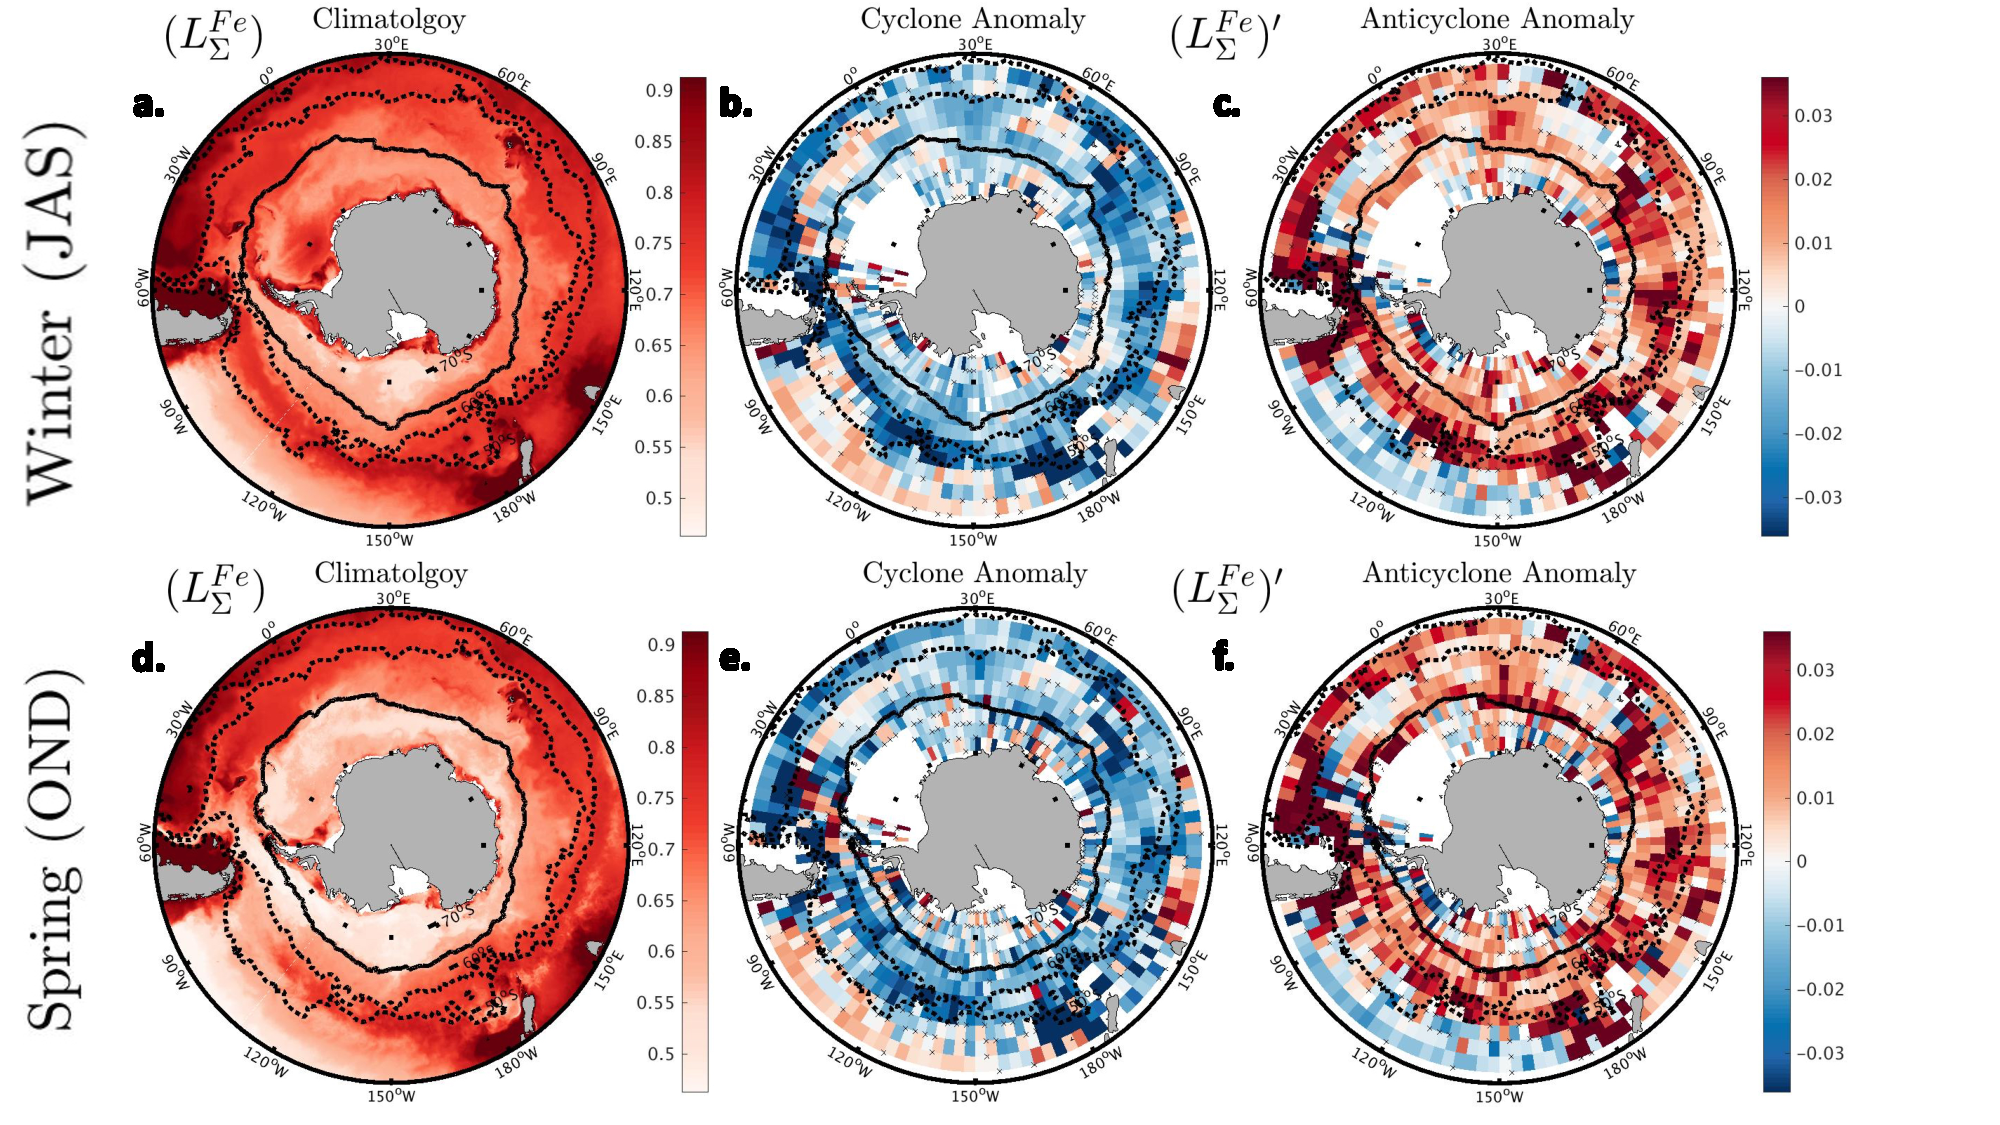
\includegraphics[scale=.5]{FigS5a.pdf} \\
        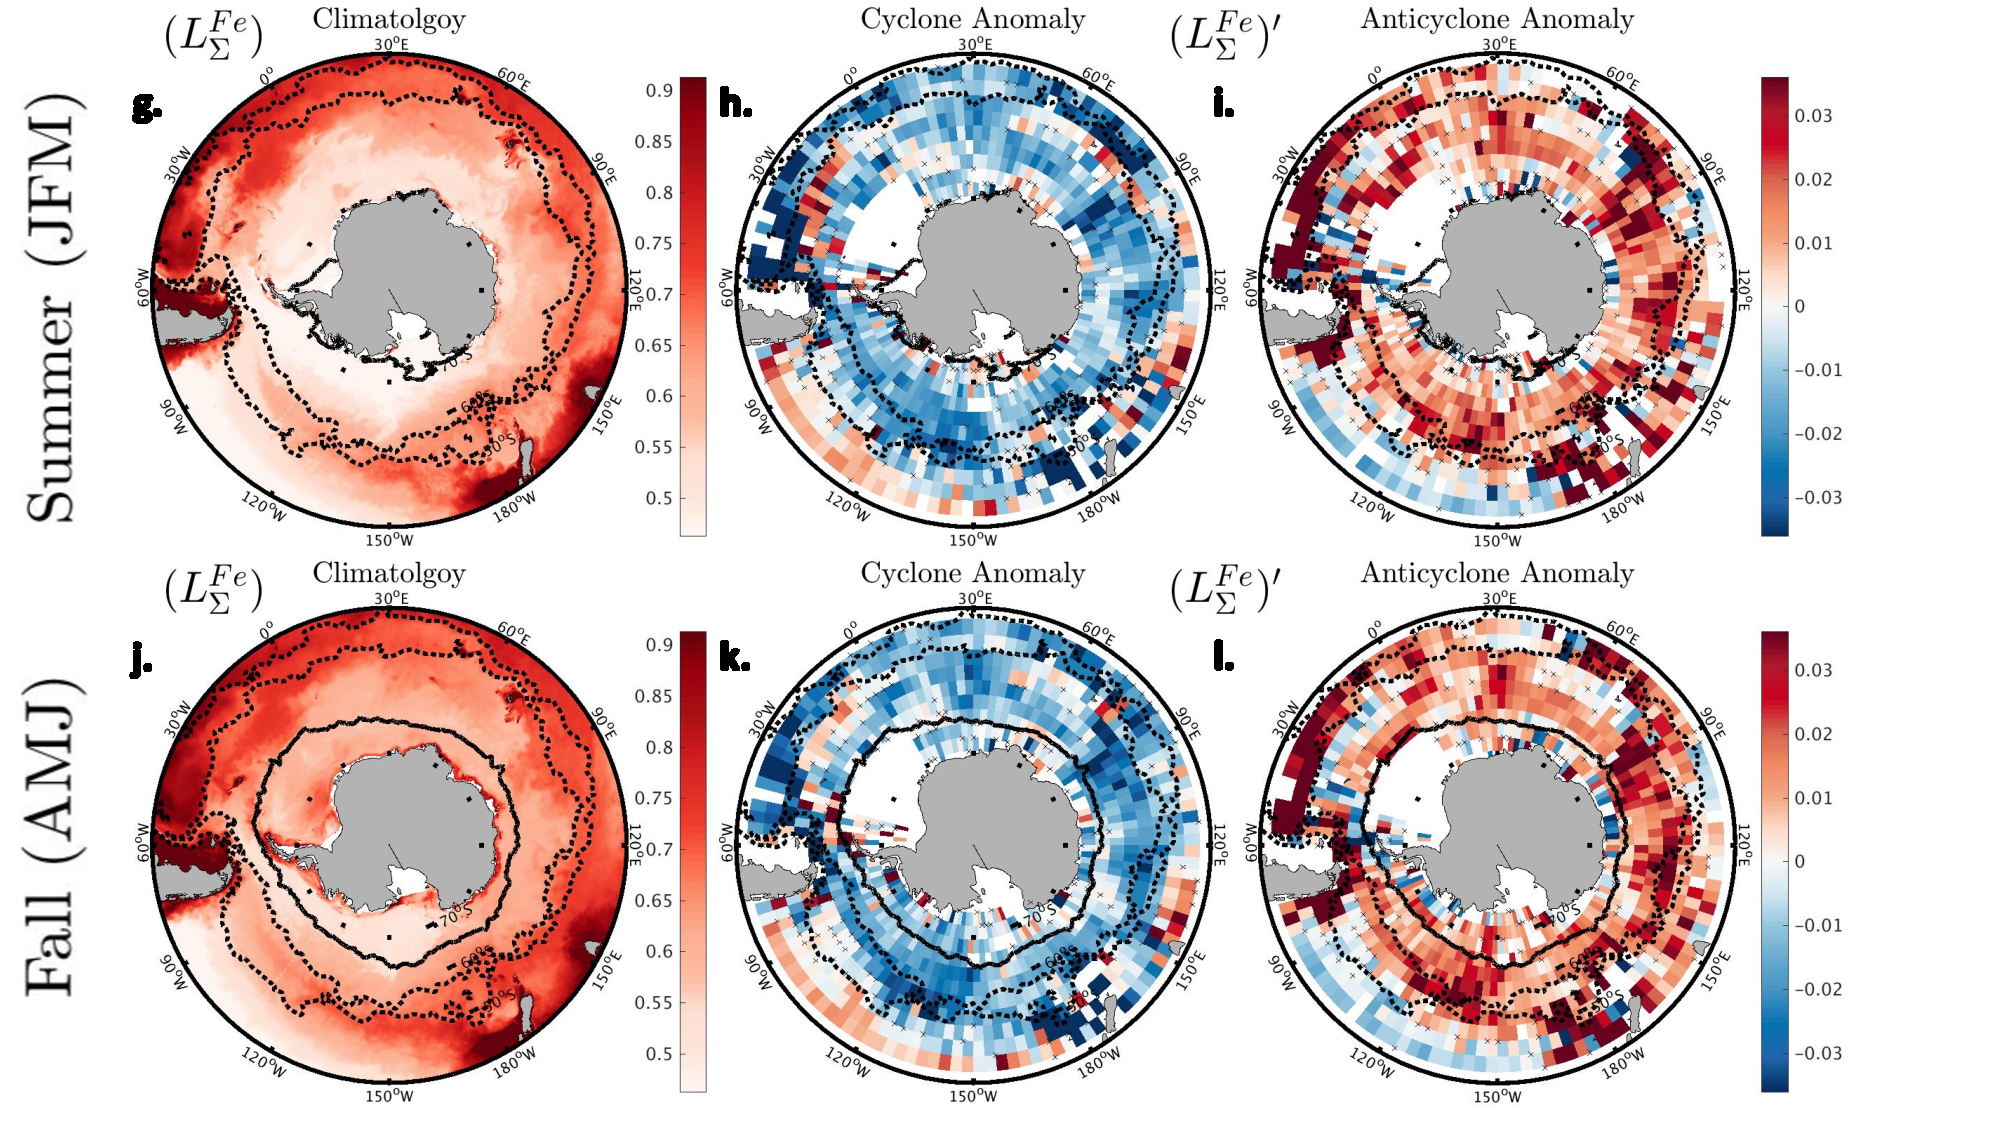
\includegraphics[scale=.5]{FigS5b.pdf} \\
  \end{tabular}
 \end{adjustwidth}
\caption[S2. Seasonal  $L_\Sigma^{Fe}'$ climatology and eddy anomalies. ]
{\textbf{Figure S2.} Seasonal  $L_\Sigma^{Fe}$ climatology and eddy anomalies. Same as \textbf{Fig. 4} except for $L_\Sigma^{Fe}$.
}
\label{fig:FigS2}
\end{figure}
   
%%%%%%%%%%%%%%%
%% Figure S3 %%
%%%%%%%%%%%%%%%

\begin{figure}[!htbp]
 \begin{adjustwidth}{-1.2in}{-1.2in}
 \centering
  \begin{tabular}{c }
        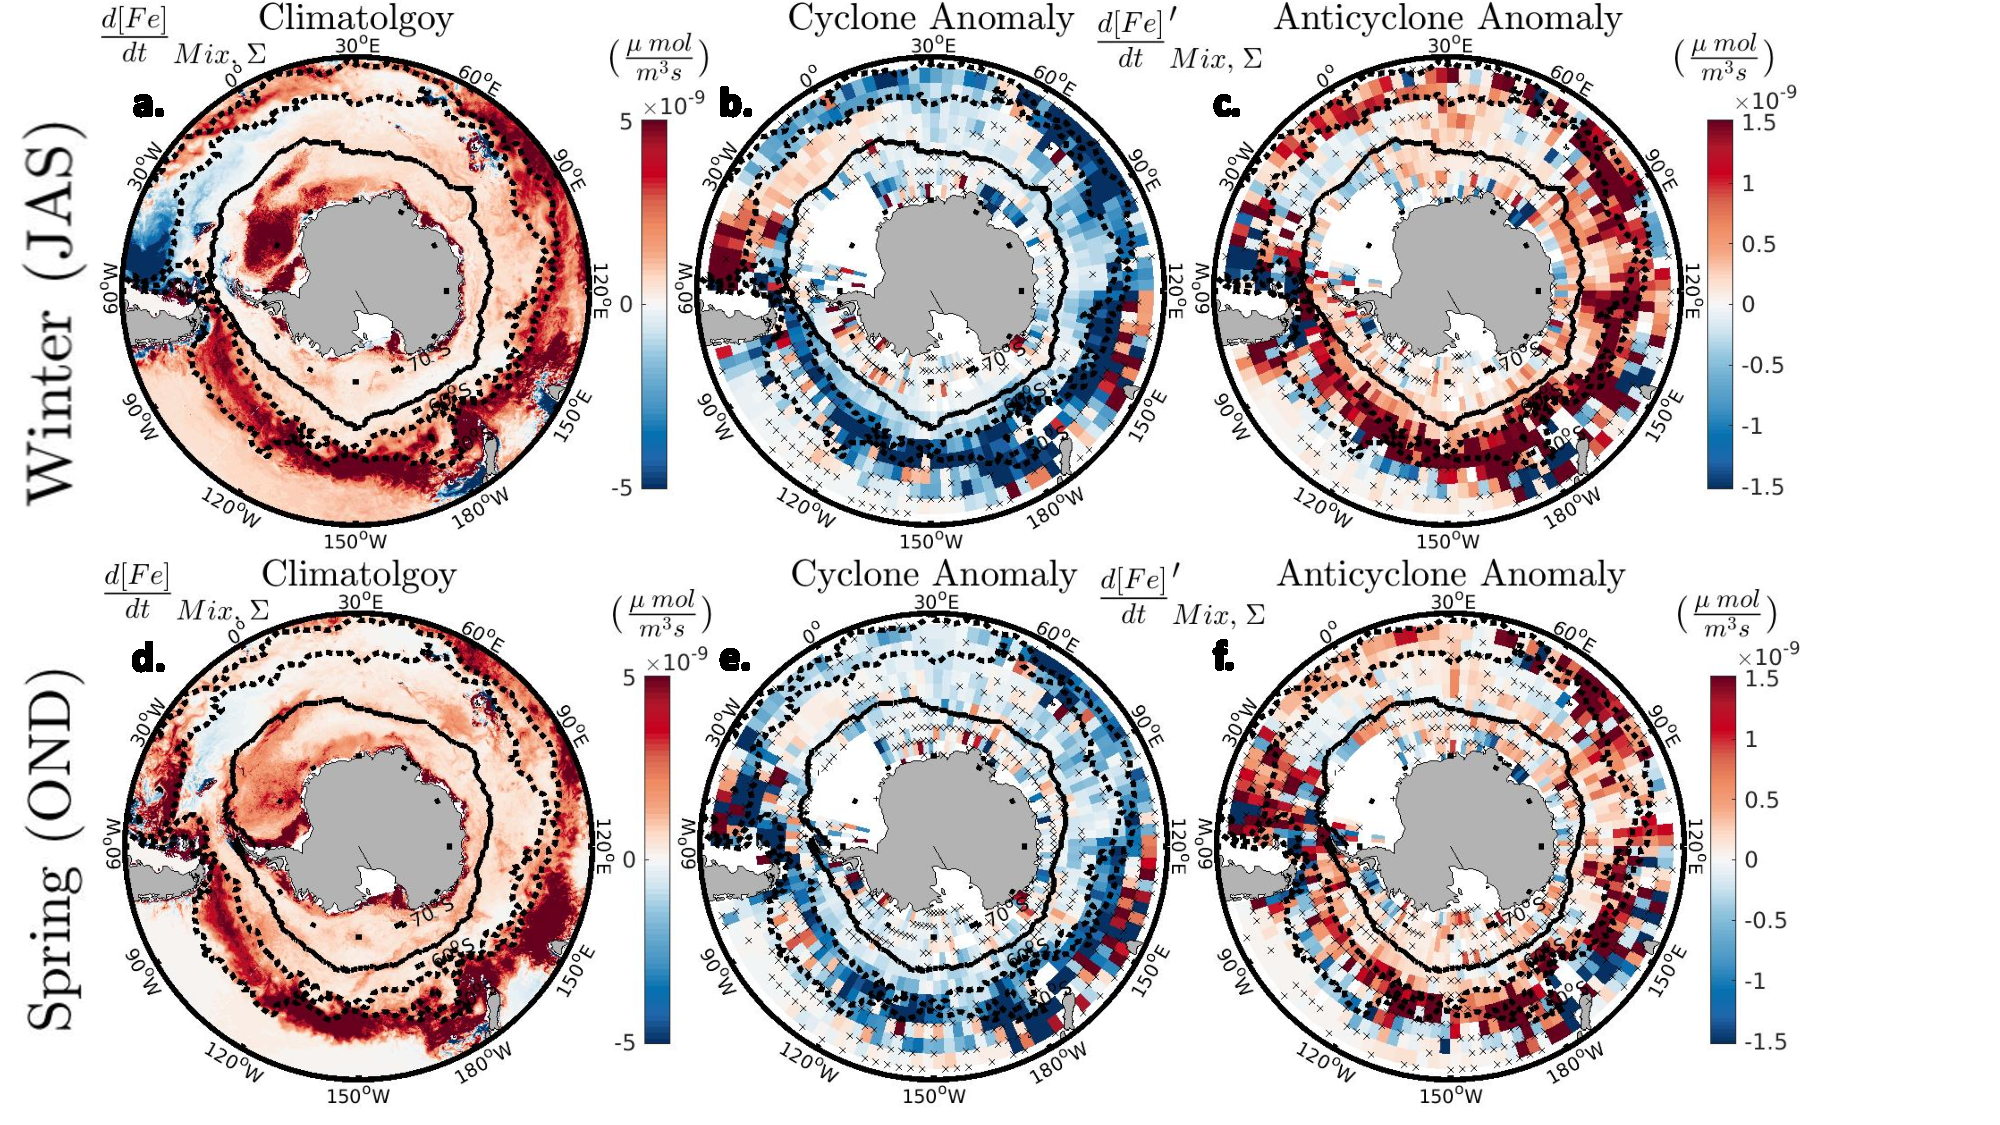
\includegraphics[scale=.5]{FigS1a.pdf} \\
        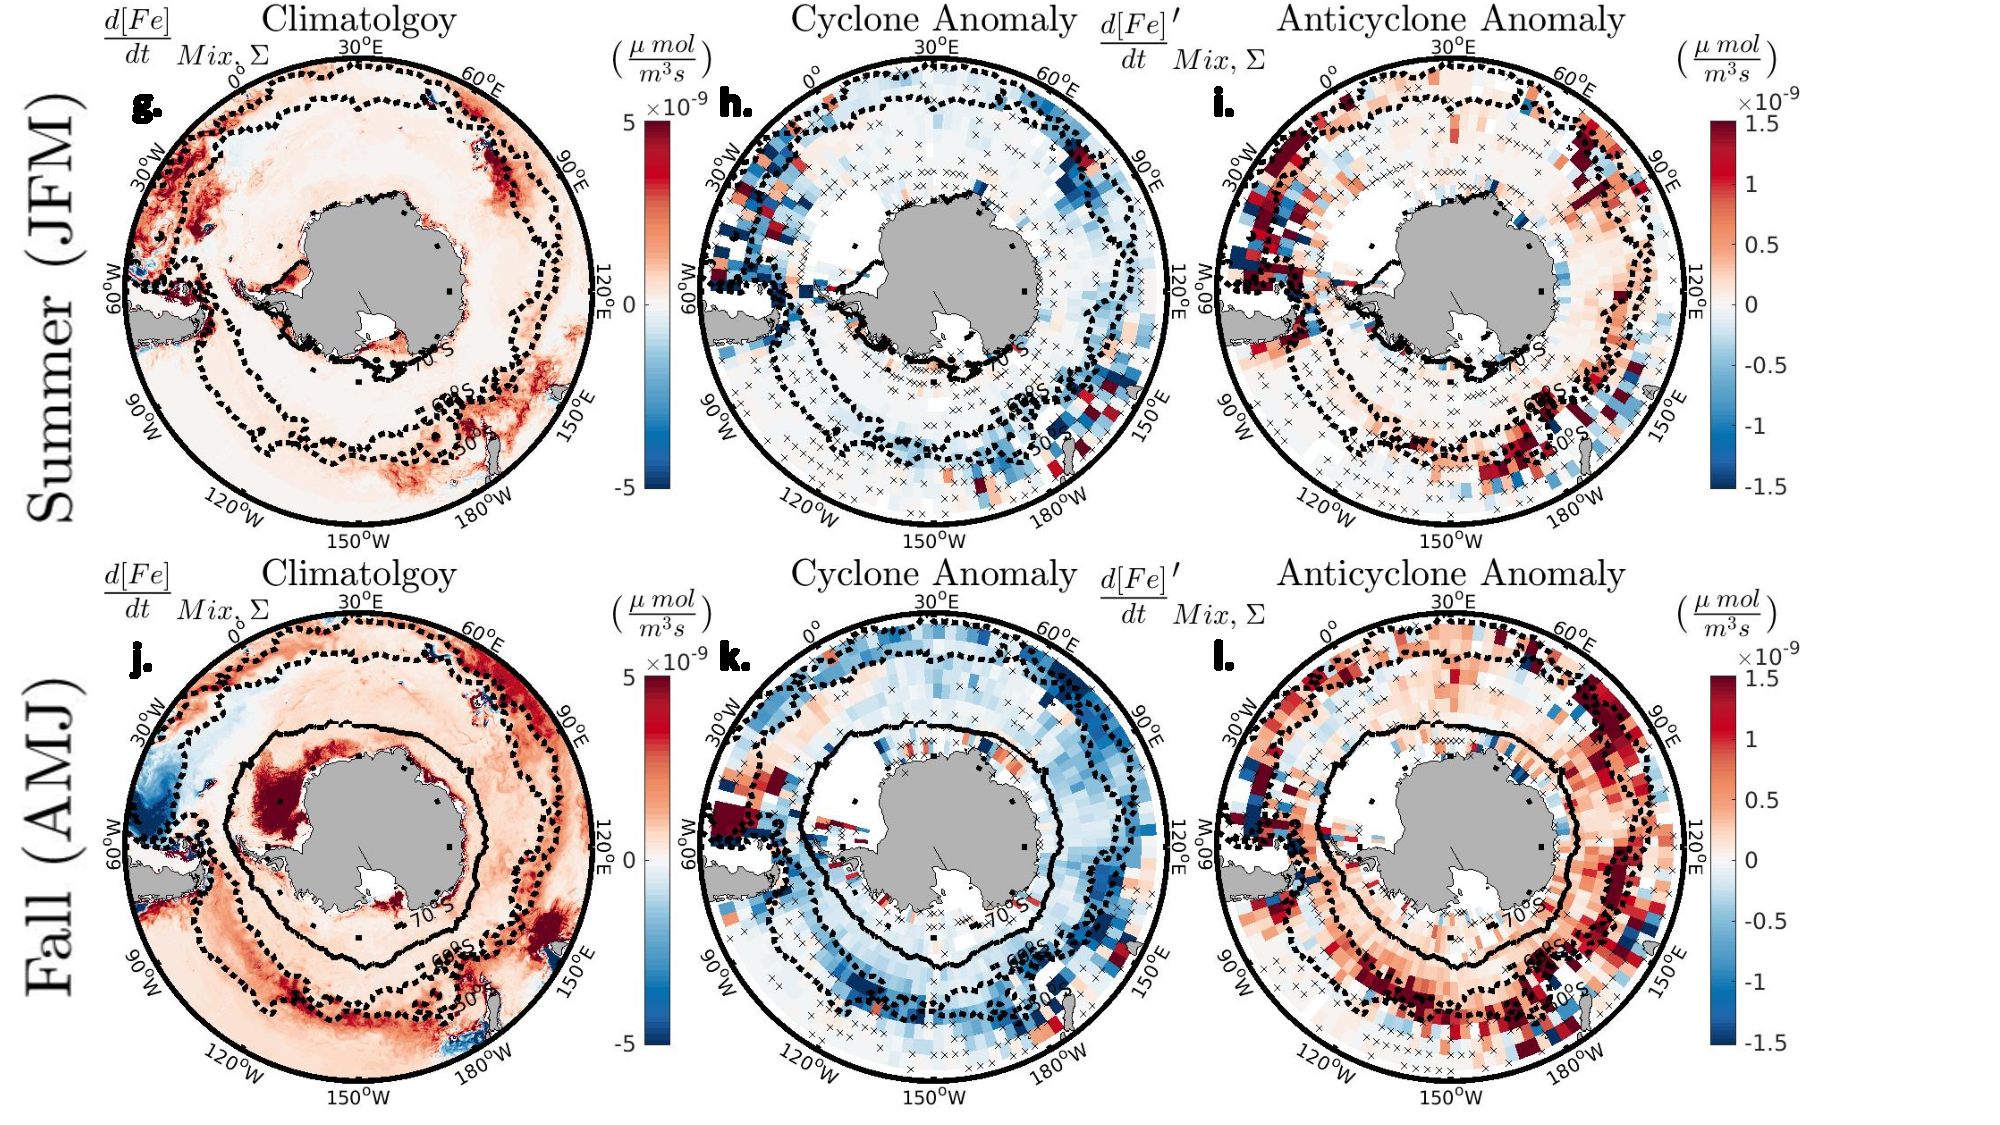
\includegraphics[scale=.5]{FigS1b.pdf} \\
  \end{tabular}
 \end{adjustwidth}
\caption[S3. Seasonal $\frac{d[Fe]}{dt}_{Mix, \Sigma}$ climatology and eddy anomalies. ]
{\textbf{Figure S3.} Seasonal $\frac{d[Fe]}{dt}_{Mix, \Sigma}$ climatology and eddy anomalies. Same as \textbf{Fig. 4} except for $\frac{d[Fe]}{dt}_{Mix, \Sigma}$.
}
\label{fig:FigS3}
\end{figure}

%%%%%%%%%%%%%%%
%% Figure S4 %%
%%%%%%%%%%%%%%%

\begin{figure}[!htbp]
 \begin{adjustwidth}{-1.2in}{-1.2in}
 \centering
  \begin{tabular}{c }
        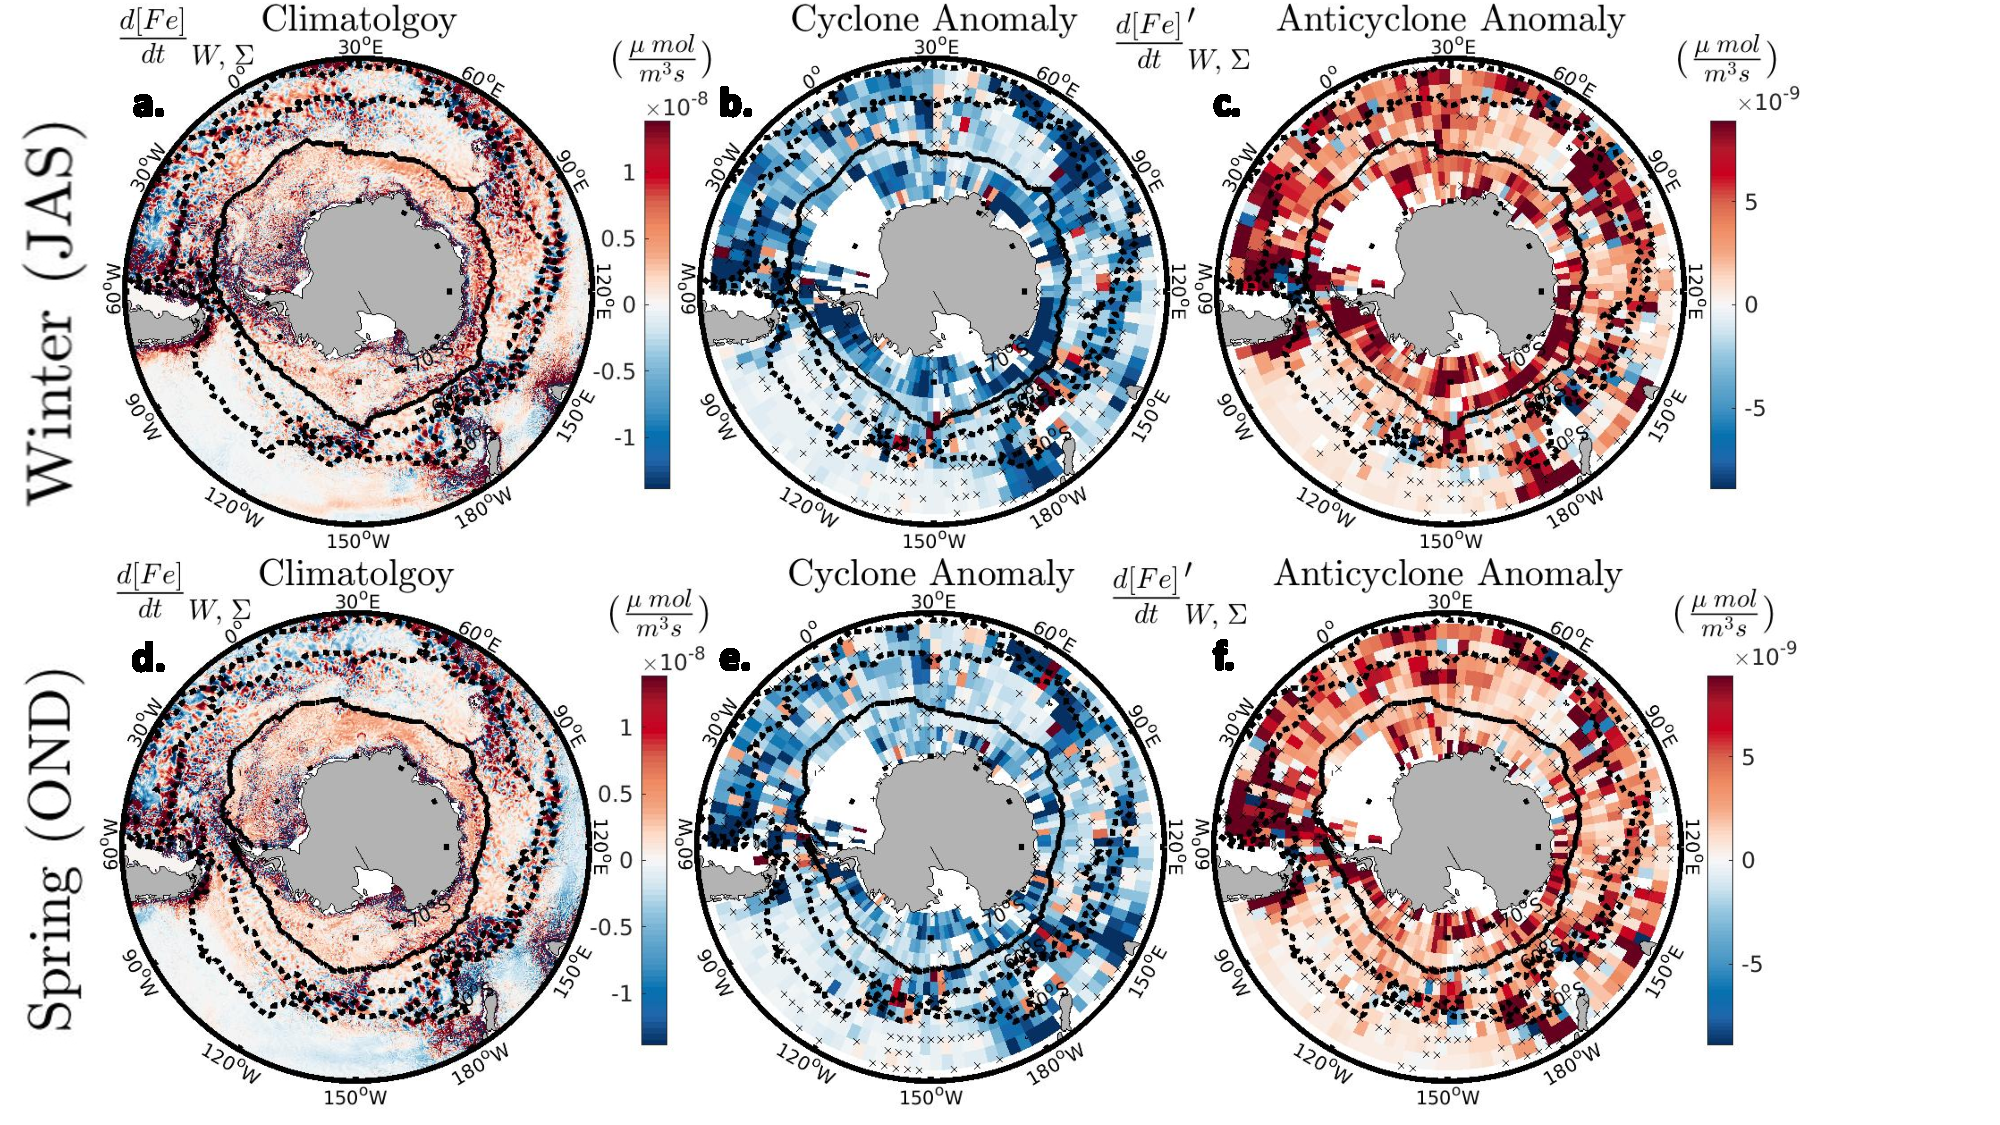
\includegraphics[scale=.5]{FigS2a.pdf} \\
        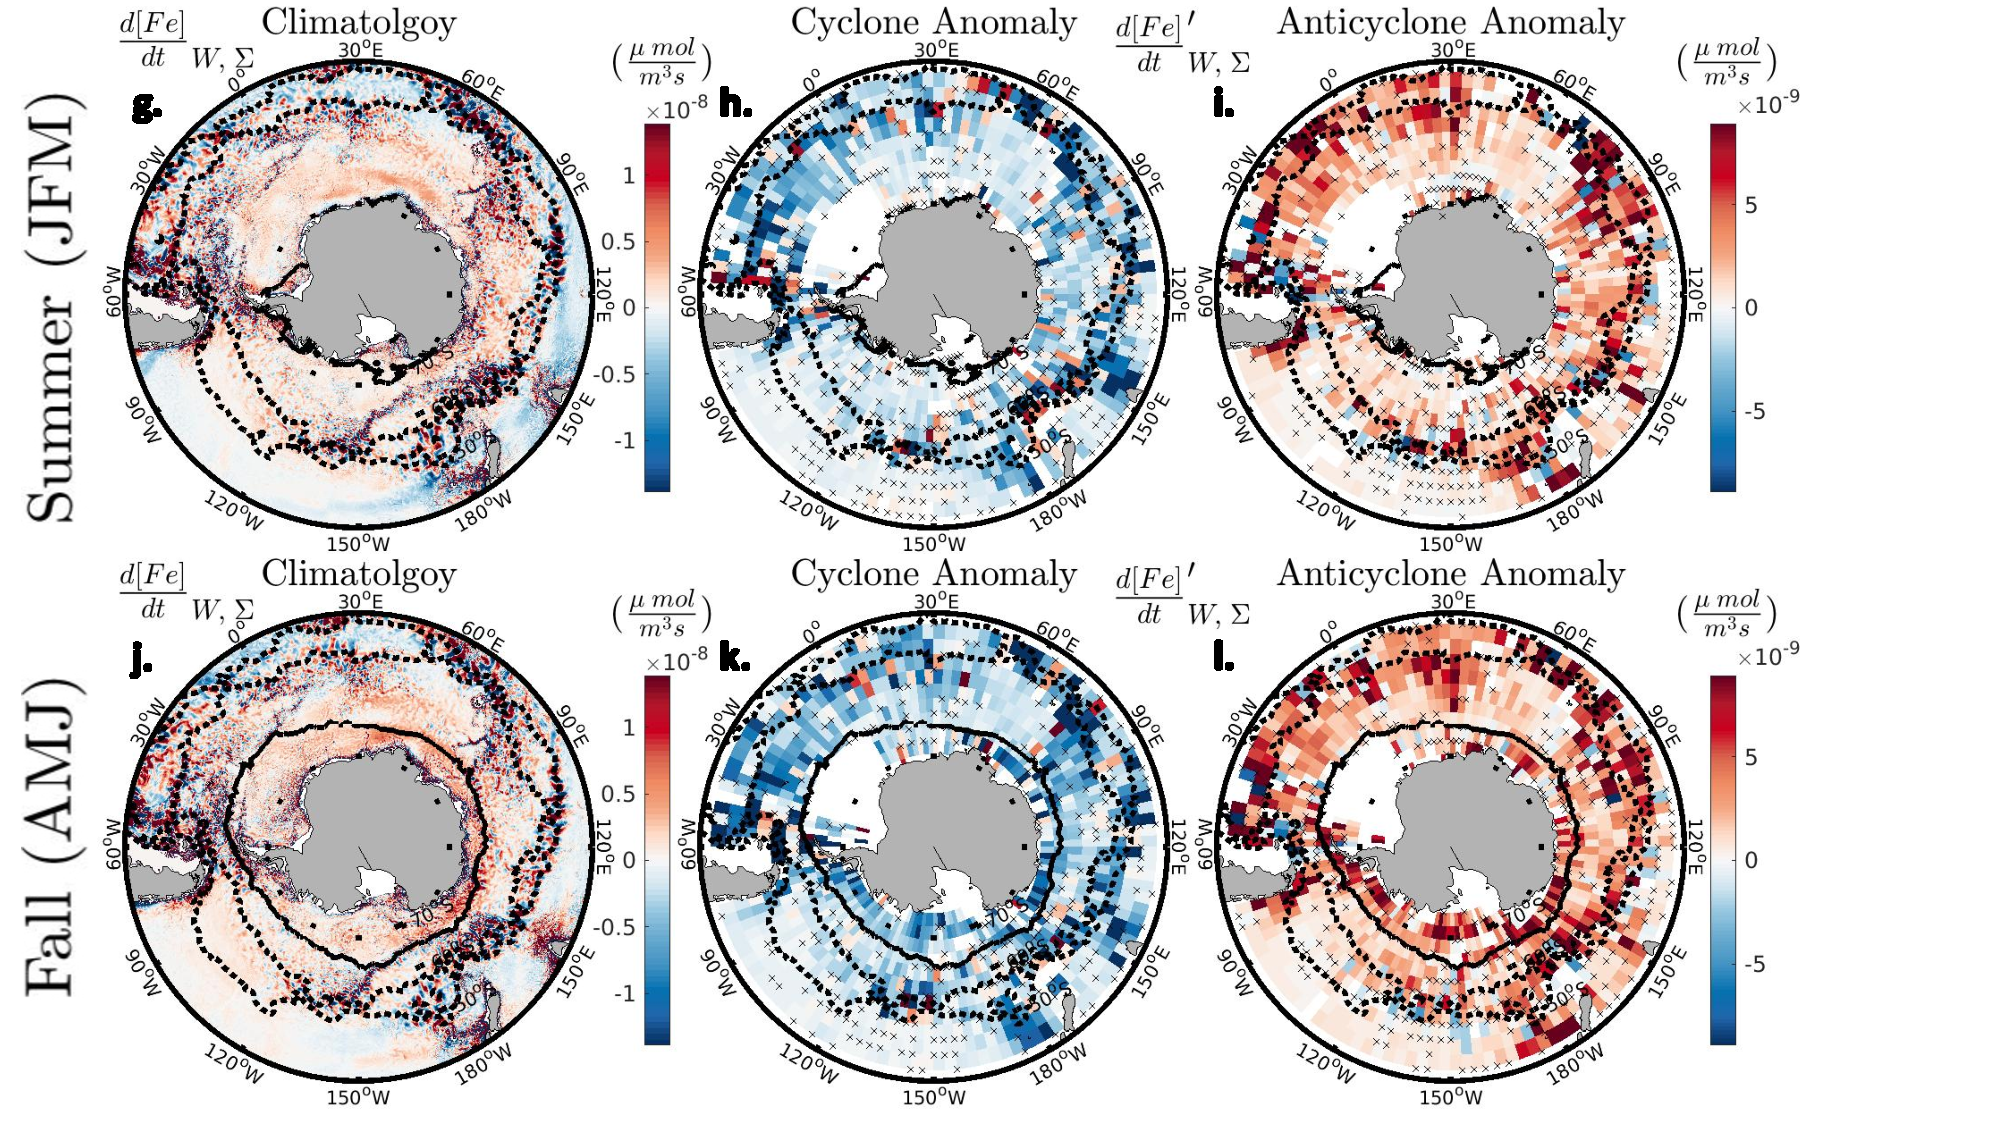
\includegraphics[scale=.5]{FigS2b.pdf} \\
  \end{tabular}
 \end{adjustwidth}
\caption[S4. Seasonal $\frac{d[Fe]}{dt}_{W, \Sigma}$ climatology and eddy anomalies. ]
{\textbf{Figure S4.} Seasonal $\frac{d[Fe]}{dt}_{W, \Sigma}$ climatology and eddy anomalies. Same as \textbf{Fig. 4} except for $\frac{d[Fe]}{dt}_{W, \Sigma}$.
}
\label{fig:FigS4}
\end{figure}

%%%%%%%%%%%%%%%
%% Figure S5 %%
%%%%%%%%%%%%%%%

\begin{figure}[!htbp]
 \begin{adjustwidth}{-1.2in}{-1.2in}
 \centering
  \begin{tabular}{c }
        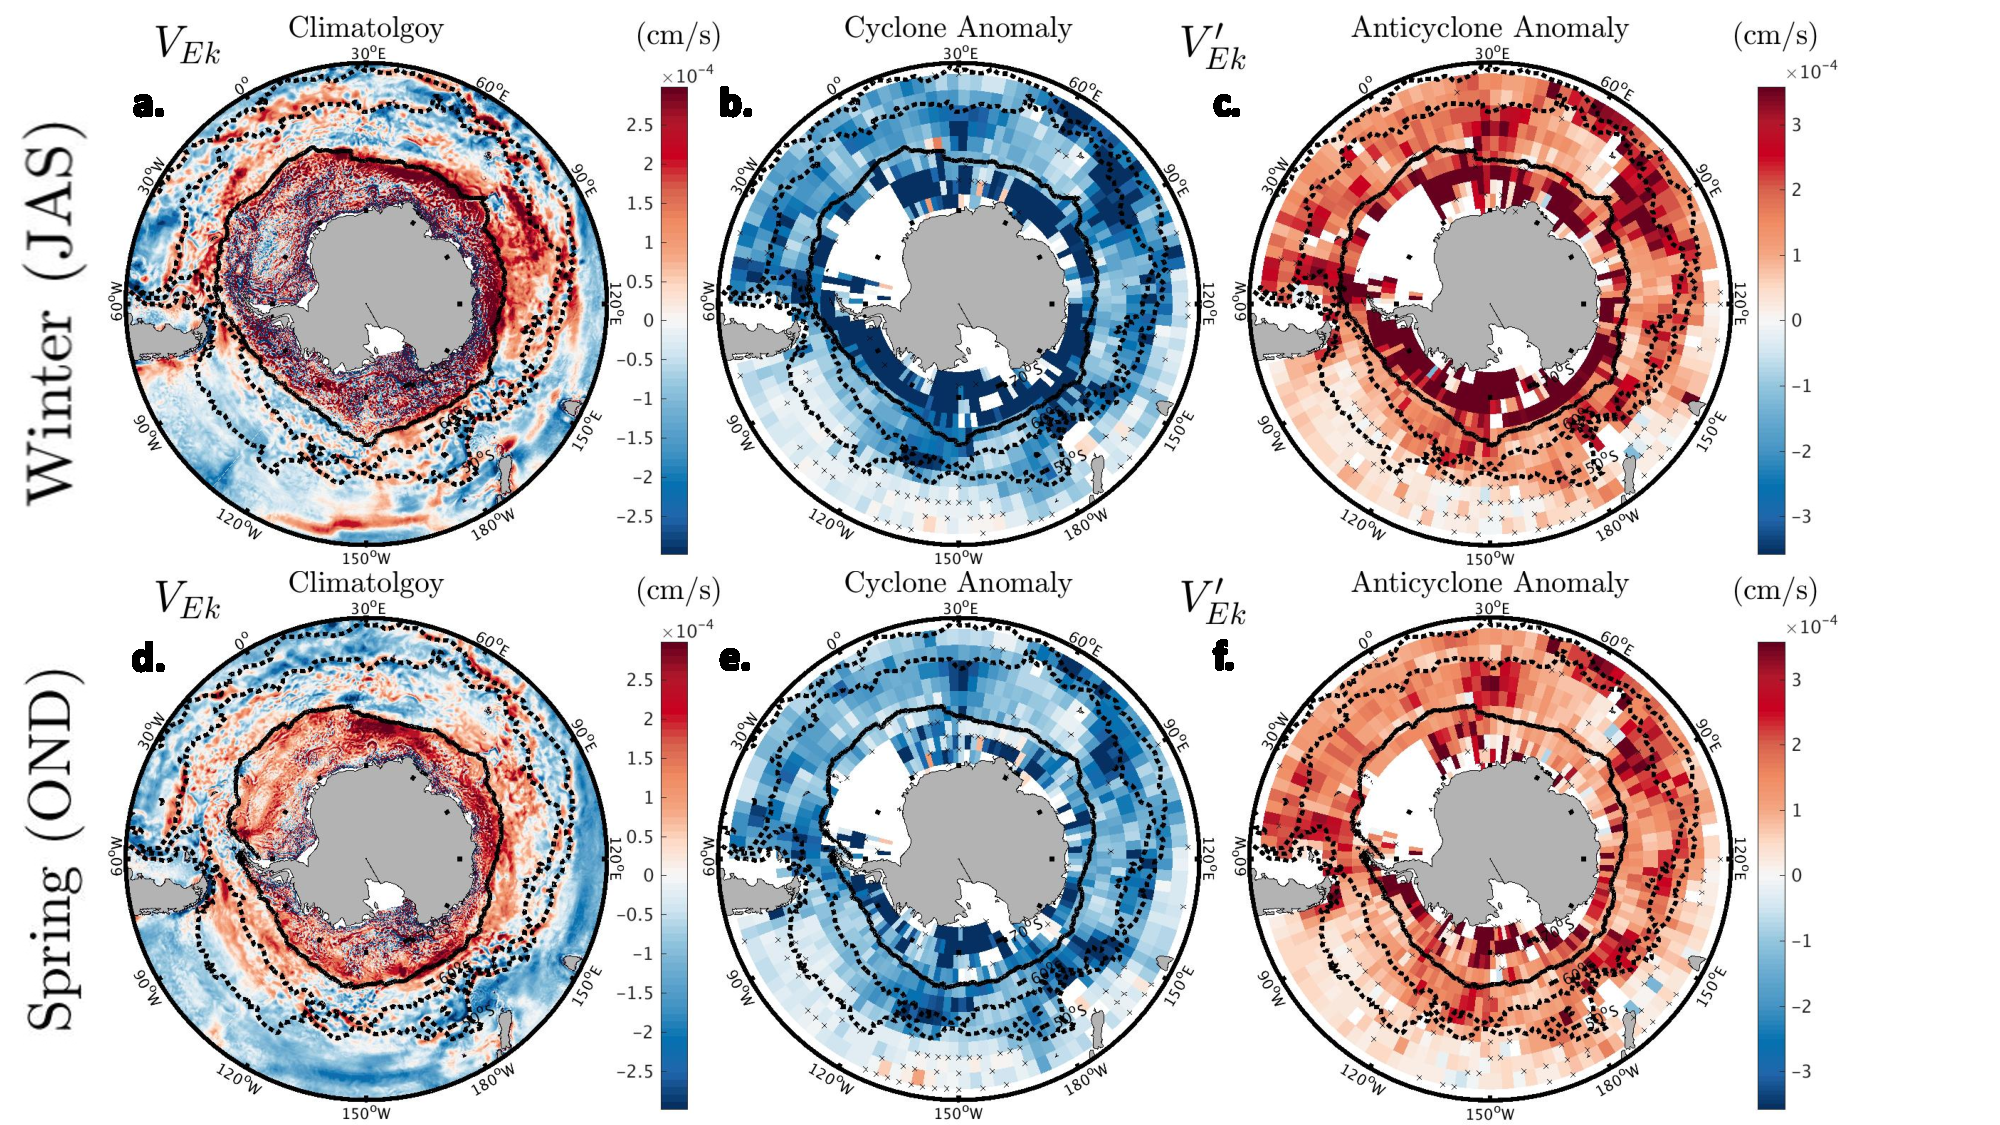
\includegraphics[scale=.5]{FigS3a.pdf} \\
        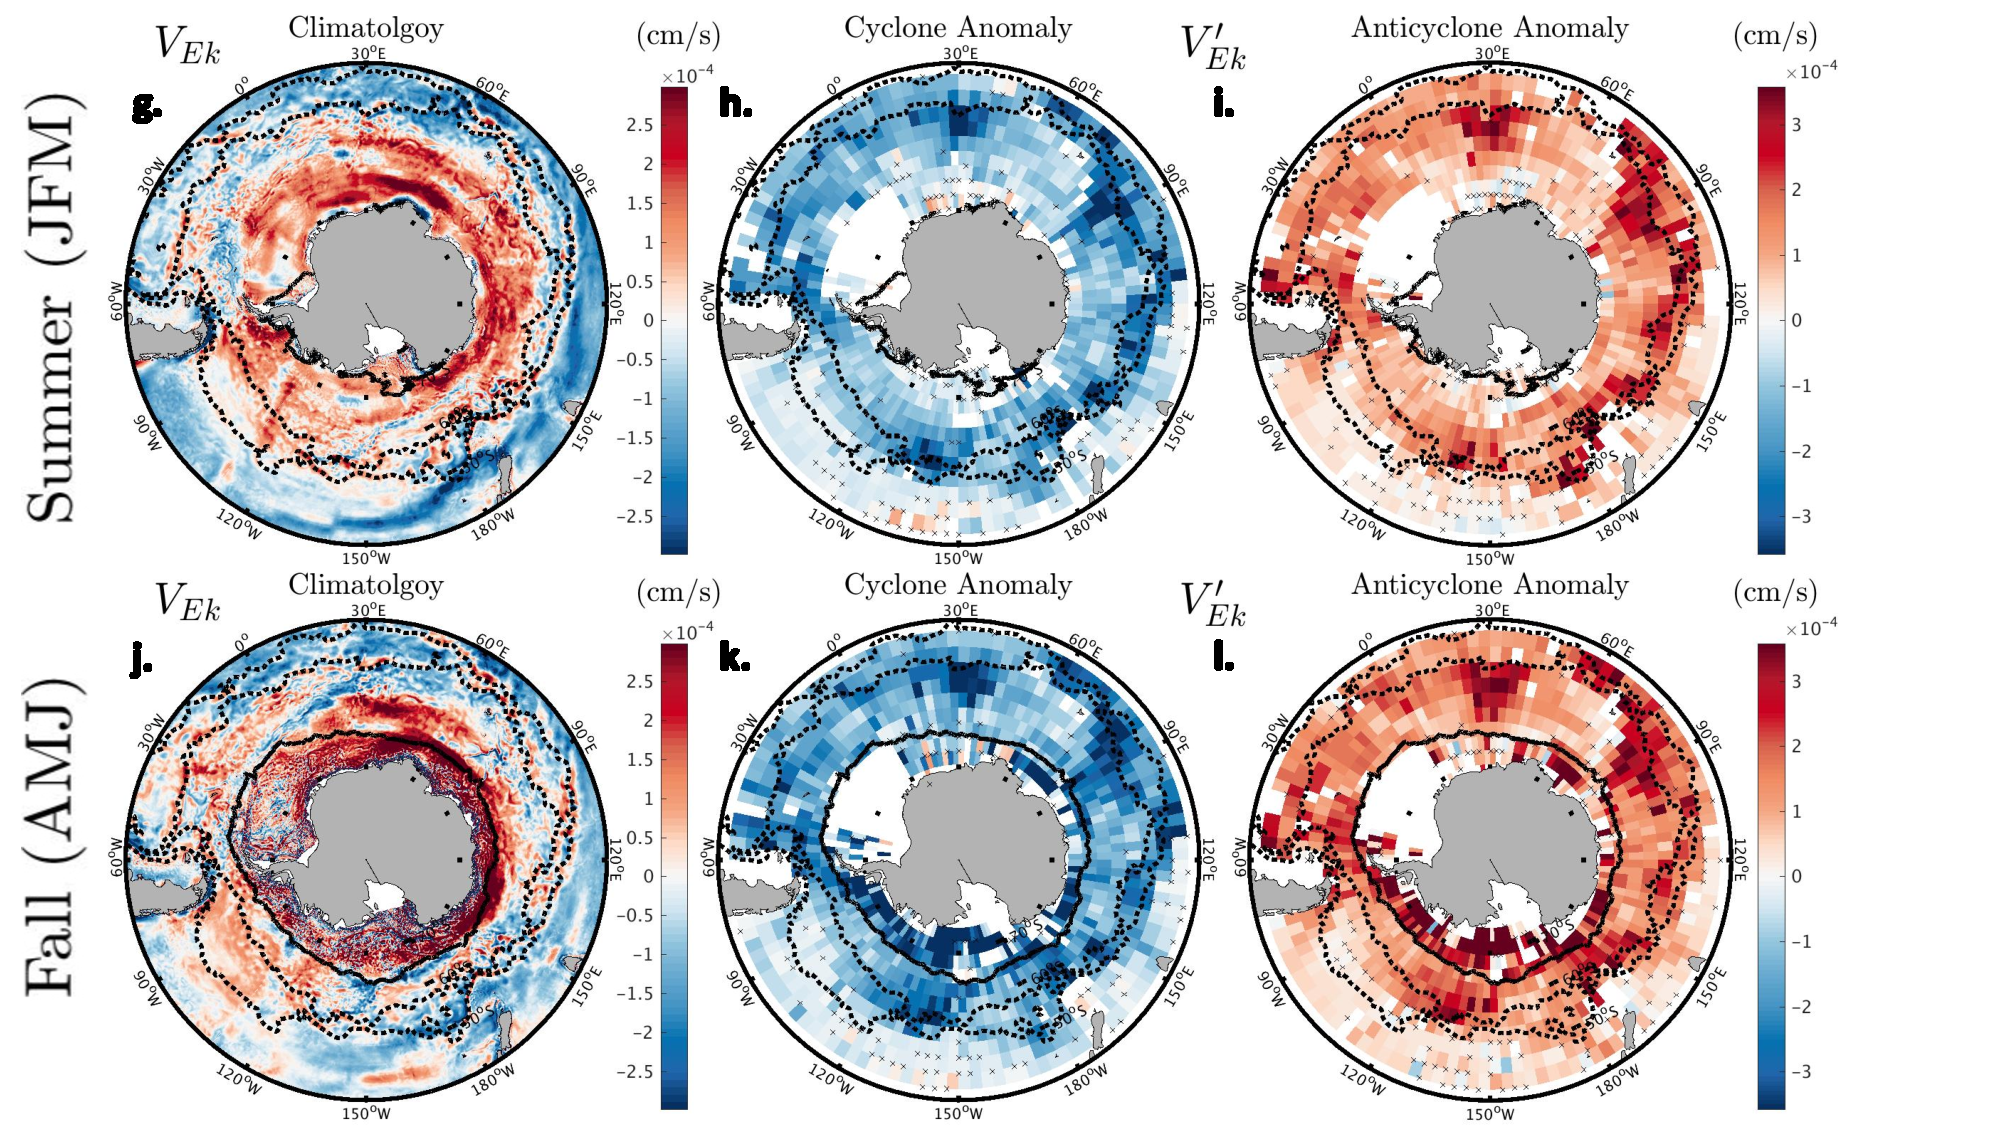
\includegraphics[scale=.5]{FigS3b.pdf} \\
  \end{tabular}
 \end{adjustwidth}
\caption[S5. Seasonal $V_{Ek}$ climatology and eddy anomalies. ]
{\textbf{Figure S5.} Seasonal $V_{Ek}$ climatology and eddy anomalies. Same as \textbf{Fig. 5} except for $V_{Ek}$.
}
\label{fig:FigS3}
\end{figure}






%%%%%%%%%%%%%%%%%%%%%%%%%%%%%%%%%%%%%%%%%%%%%%%%%%%%
                      %% Tables %%
%%%%%%%%%%%%%%%%%%%%%%%%%%%%%%%%%%%%%%%%%%%%%%%%%%%%

%%%%%%%%%%%%%%%
%%  Table 1  %%
%%%%%%%%%%%%%%%
\definecolor{lightblue}{RGB}{153,205,255}
\definecolor{lightred}{RGB}{255,153,153}


\begin{table}[!htbp]
\begin{adjustwidth}{-1.2in}{-1.2in}
\renewcommand{\arraystretch}{3.2}
\centering

\scalebox{0.8}{
\begin{tabular}{ c |  c || c || c | c ||  c | c ||c | c | c | c | c || c | c || c | c | }

\multicolumn{3}{c}{} & \multicolumn{6}{c}{\huge{Cyclones}} & \multicolumn{1}{c}{} &  \multicolumn{6}{c}{\huge{Antiyclones}}\\

%\multicolumn{3}{c}{} & %\multicolumn{6}{c}{\Large{Subset}}& %\multicolumn{1}{c}{}&
%\multicolumn{6}{c}{\Large{Subset}}\\

\hhline{~|~||~||-|-||-|-||-|-~-|-||-|-||-|-}

\multicolumn{3}{c|}{} &
\multicolumn{2}{|c||}{\large{Large \& Deep}} & \multicolumn{2}{|c||}{\large{All}} & \multicolumn{2}{|c|}{\large{Small \& Shallow}} & &
\multicolumn{2}{|c||}{\large{Large \& Deep}} & \multicolumn{2}{|c||}{\large{All}} & \multicolumn{2}{|c|}{\large{Small \& Shallow}}\\


\hhline{~|-|-|-|-||-|-||-|-~-|-||-|-||-|-}
& \multicolumn{2}{|c|}{Realizations} &
\multicolumn{2}{|c||}{9364(6.5\%)} &\multicolumn{2}{|c||}{143570(100\%)} & \multicolumn{2}{|c|}{44507(31\%)} & & \multicolumn{2}{|c||}{9910(6.9\%)} & \multicolumn{2}{|c||}{144550(100\%)} & \multicolumn{2}{|c|}{58086(40\%)} \\

\hhline{~|-|-|-|-||-|-||-|-~-|-||-|-||-|-}
& \multicolumn{2}{|c|}{Unique Tracks} &
\multicolumn{2}{|c||}{1188(18\%)} &\multicolumn{2}{|c||}{6672(100\%)} & \multicolumn{2}{|c|}{5238(79\%)} & & \multicolumn{2}{|c||}{1179(17\%)} & \multicolumn{2}{|c||}{6742(100\%)} & \multicolumn{2}{|c|}{5282(78\%)} \\
\hhline{~|-|-|-|-||-|-||-|-~-|-||-|-||-|-}

\multicolumn{16}{c}{\huge{\quad \quad Statistical distribution of eddy anomalies}} \\

\hhline{~|~||~||-|-||-|-||-|-~-|-||-|-||-|-}
\multicolumn{3}{c|}{} &
\large{$freq$} & \large{$mean$} & \large{$freq$} & \large{$mean$} & \large{$freq$} & \large{$mean$} & & \large{$freq$} & \large{$mean$} & \large{$freq$} & \large{$mean$} & \large{$freq$} & \large{$mean$} \\
\hhline{~:-::-::==::==::==~==::==::==}
%%%%%%%%%
\multirow{11}{1em}{\rotatebox{90}{\huge{Variables}}}& 
\multirow{2}{1em}{\rotatebox{90}{\large{$MLD' \; (m)$}}} & $+$ & \rowcolor{lightred} 28\% & 9.9(7.6) & 50\% & 4.9(6.8) & 57\% & 4.5(7.7) & \cellcolor{white} & 78\% & 27(18) & 51\%  & 7.8(9.0) & 42\% & 4.1(7.5) \\  

\hhline{~|~||-||-|-||-|-||-|-~-|-||-|-||-|-}

& & $-$ & \rowcolor{lightblue} 72\% & -29(-16) & 50\% & -7.9(-8.6) & 43\% & -4.3(-7.7) & \cellcolor{white} & 22\% & -7.2(-5.6) & 49\%  & -4.7(-6.8)  & 58\% &  -5.1(-8.3) \\  

\hhline{~:=::=::==::==::==~==::==::==}
%%%%%%%%%
& \multirow{2}{1em}{\rotatebox{90}{\large{$ L^{I_{PAR}}_\Sigma'$}}} & $+$ & \rowcolor{lightred} 80\% & 1.6e-2(11) & 46\% & 9.1e-3(4.7) & 34\% & 8.8e-3(4.7) & \cellcolor{white}& 14\% & 5.2e-3(3.6) & 51\% & 7.9e-3(4.2) & 64\% & 9.9e-3(5.8)  \\ 

\hhline{~|~||-||-|-||-|-||-|-~-|-||-|-||-|-}

& & $-$ & \rowcolor{lightblue} 20\% & -6.8e-3(-4.7) & 54\% & -7.8e-3(-4.2) & 66\% & -9.6e-3(-5.3) & \cellcolor{white} & 86\% & -1.6e-2(-10) & 49\%  & -8.8e-3(-4.6) & 36\% & -7.7e-3(-4.0)  \\ 

\hhline{~:=::=::==::==::==~==::==::==}
%%%%%%%%%
& \multirow{2}{1em}{\rotatebox{90}{\large{$[Fe'_\Sigma] \; (\frac{\mu mol}{m^3})$}}} & $+$ & \rowcolor{lightred} 11\% & 4.4e-2(14)  & 27\% & 1.1e-2(8.4) & 31\% & 7.2e-3(8.0) & \cellcolor{white}& 91\% & 2.1e-2(14)  & 71\% & 1.4e-2(12) & 66\% & 9.9e-3(11)  \\ 

\hhline{~|~||-||-|-||-|-||-|-~-|-||-|-||-|-}

& & $-$ & \rowcolor{lightblue} 89\% & -1.9e-2(-11)  & 73\% & -1.4e-2(-10) & 69\% & -9.4e-3(-9.2) & \cellcolor{white} & 9\% & -3.4e-2(-5.6)  & 28\%  & -1.1e-2(-7.7) & 34\% & -7.9e-3(-8.2)  \\ 

\hhline{~:=::=::==::==::==~==::==::==}
%%%%%%%%%
& \multirow{2}{1em}{\rotatebox{90}{\large{$ L^{Fe}_\Sigma'$}}} & $+$ & \rowcolor{lightred} 11\% & 1.6e-2(2.0) & 26\% & 1.3e-2(2.1) & 30\% & 1.4e-2(2.4) & \cellcolor{white}& 92\% & 2.1e-2(2.8) & 72\% & 1.9e-2(3.1) & 68\% & 1.9e-2(3.3)  \\ 

\hhline{~|~||-||-|-||-|-||-|-~-|-||-|-||-|-}

& & $-$ & \rowcolor{lightblue} 89\% & -2.0e-2(-2.7) & 74\% & -1.8e-2(-2.9) & 70\% & -1.8e-2(-3.1) & \cellcolor{white} & 8\% & -4.9e-3(-0.6) & 28\%  & -1.2e-2(-2.2)-2.2 & 33\% & -1.4e-2(-2.5)  \\ 

\hhline{~:=::=::==::==::==~==::==::==}
%%%%%%%%%
& \multirow{2}{1em}{\rotatebox{90}{\large{$\mu'_\Sigma \; (d^{-1})$}}} & $+$ & \rowcolor{lightred} 45\% & 8.1e-3(7.2) & 22\% & 5.8e-3(5.0) & 21\% & 5.0e-3(7.2) & \cellcolor{white} & 51\% & 3.8e-3(4.4) & 77\%  & 8.7e-3(7.0) & 78\% & 7.8e-3(8.2) \\  

\hhline{~|~||-||-|-||-|-||-|-~-|-||-|-||-|-}

& & $-$ & \rowcolor{lightblue} 55\% & -4.3e-3(-4.5) & 78\% & -8.5e-3(-6.7) & 79\% & -7.7e-3(-8.4) & \cellcolor{white} & 49\% & -7.6e-3(-4.5) & 23\%  & -5.4e-3(-6.4) & 22\% &  -4.7e-3(-10) \\ 



% Comments out transport terms

%\hhline{~:=::=::==::==::==~==::==::==}
%%%%%%%%%
%& \multirow{2}{1em}{\rotatebox{90}{\large{$\frac{d[Fe_\Sigma]}{dt}'_M \; (\frac{\mu mol}{m^3 \; s})$}}} & $+$ & \rowcolor{lightred} 17\% & 1.3e-9 & 28\% & 5.4e-10 & 31\% &  3.5e-10  &  \cellcolor{white}& 81\% & 1.4e-9 & 68\% & 6.2e-10 & 63\% & 4.0e-10  \\ 

%\hhline{~|~||-||-|-||-|-||-|-~-|-||-|-||-|-}

%& & $-$ & \rowcolor{lightblue} 83\% & -1.2e-9(-58) & 72\% & -5.4e-10 & 69\% & -3.5e-10 & \cellcolor{white} & 19\% & -1.8e-9 & 32\%  & -5.6e-10 & 37\% &  -4.0e-10 \\ 

%\hhline{~:=::=::==::==::==~==::==::==}
%%%%%%%%%
%& \multirow{2}{1em}{\rotatebox{90}{\large{$\frac{d[Fe_\Sigma]}{dt}'_A \; (\frac{\mu mol}{m^3 \; s})$}}} & $+$ & \rowcolor{lightred} 26\% & 2.7e-9 & 26\% & 2.7e-  & 26\% & 2.5e-9  & \cellcolor{white}& 77\% & 5.3e-9 & 75\% & 4.4e-9 & 74\% & 4.7e-9  \\ 

%\hhline{~|~||-||-|-||-|-||-|-~-|-||-|-||-|-}

%& & $-$ & \rowcolor{lightblue} 74\% & -4.6e-9 & 74\% & -4.4e-9 & 74\% & -4.3e-9 & \cellcolor{white} & 23\% & -3.1e-9 & 25\%  & -2.5e-9 & 26\% &  -2.3e-9 \\ 
%%%%%%%%%


\hhline{~|-||-||-|-||-|-||-|-~-|-||-|-||-|-}


\end{tabular}
}
\end{adjustwidth}

\caption[Frequency and magnitude of eddy anomalies]
{\textbf{Table 1}. Frequency and Magnitude of eddy anomalies. The percent of cyclones (left table) and anticyclones (right table) with positive or negative anomalies is reported along with the mean values of anomalies exclusively from eddies with a + or - anamaly. In parenthensis the mean of the normalized anomalies, which is expressed as a percentage of the co-located climatology. Statistics are report for all Southern Ocean Eddies in addition to two subsets delineated based on size (Large: $L_S>50km$ \& $Amplitude>5cm$ | Small: $L_S<50km$ \& $Amplitude < 10cm$) and background mixing (Deep: $MLD_{clim}>100m $ | Shallow: $MLD_{clim}<100m $). The number (and \%) of individual realization in each subset is provided above in addition to the number of unique eddy tracks that they come from.  Note that not all realizations in a given track are represented in a particular subset.  

}

\label{tab:Tab1}
\end{table}




\end{document}